\documentclass[]{book}
\usepackage{lmodern}
\usepackage{amssymb,amsmath}
\usepackage{ifxetex,ifluatex}
\usepackage{fixltx2e} % provides \textsubscript
\ifnum 0\ifxetex 1\fi\ifluatex 1\fi=0 % if pdftex
  \usepackage[T1]{fontenc}
  \usepackage[utf8]{inputenc}
\else % if luatex or xelatex
  \ifxetex
    \usepackage{mathspec}
  \else
    \usepackage{fontspec}
  \fi
  \defaultfontfeatures{Ligatures=TeX,Scale=MatchLowercase}
\fi
% use upquote if available, for straight quotes in verbatim environments
\IfFileExists{upquote.sty}{\usepackage{upquote}}{}
% use microtype if available
\IfFileExists{microtype.sty}{%
\usepackage{microtype}
\UseMicrotypeSet[protrusion]{basicmath} % disable protrusion for tt fonts
}{}
\usepackage{hyperref}
\hypersetup{unicode=true,
            pdftitle={A Tour of the Generalized Lotka-Volterra Model},
            pdfauthor={Stefano Allesina},
            pdfborder={0 0 0},
            breaklinks=true}
\urlstyle{same}  % don't use monospace font for urls
\usepackage{natbib}
\bibliographystyle{apalike}
\usepackage{color}
\usepackage{fancyvrb}
\newcommand{\VerbBar}{|}
\newcommand{\VERB}{\Verb[commandchars=\\\{\}]}
\DefineVerbatimEnvironment{Highlighting}{Verbatim}{commandchars=\\\{\}}
% Add ',fontsize=\small' for more characters per line
\usepackage{framed}
\definecolor{shadecolor}{RGB}{248,248,248}
\newenvironment{Shaded}{\begin{snugshade}}{\end{snugshade}}
\newcommand{\AlertTok}[1]{\textcolor[rgb]{0.94,0.16,0.16}{#1}}
\newcommand{\AnnotationTok}[1]{\textcolor[rgb]{0.56,0.35,0.01}{\textbf{\textit{#1}}}}
\newcommand{\AttributeTok}[1]{\textcolor[rgb]{0.77,0.63,0.00}{#1}}
\newcommand{\BaseNTok}[1]{\textcolor[rgb]{0.00,0.00,0.81}{#1}}
\newcommand{\BuiltInTok}[1]{#1}
\newcommand{\CharTok}[1]{\textcolor[rgb]{0.31,0.60,0.02}{#1}}
\newcommand{\CommentTok}[1]{\textcolor[rgb]{0.56,0.35,0.01}{\textit{#1}}}
\newcommand{\CommentVarTok}[1]{\textcolor[rgb]{0.56,0.35,0.01}{\textbf{\textit{#1}}}}
\newcommand{\ConstantTok}[1]{\textcolor[rgb]{0.00,0.00,0.00}{#1}}
\newcommand{\ControlFlowTok}[1]{\textcolor[rgb]{0.13,0.29,0.53}{\textbf{#1}}}
\newcommand{\DataTypeTok}[1]{\textcolor[rgb]{0.13,0.29,0.53}{#1}}
\newcommand{\DecValTok}[1]{\textcolor[rgb]{0.00,0.00,0.81}{#1}}
\newcommand{\DocumentationTok}[1]{\textcolor[rgb]{0.56,0.35,0.01}{\textbf{\textit{#1}}}}
\newcommand{\ErrorTok}[1]{\textcolor[rgb]{0.64,0.00,0.00}{\textbf{#1}}}
\newcommand{\ExtensionTok}[1]{#1}
\newcommand{\FloatTok}[1]{\textcolor[rgb]{0.00,0.00,0.81}{#1}}
\newcommand{\FunctionTok}[1]{\textcolor[rgb]{0.00,0.00,0.00}{#1}}
\newcommand{\ImportTok}[1]{#1}
\newcommand{\InformationTok}[1]{\textcolor[rgb]{0.56,0.35,0.01}{\textbf{\textit{#1}}}}
\newcommand{\KeywordTok}[1]{\textcolor[rgb]{0.13,0.29,0.53}{\textbf{#1}}}
\newcommand{\NormalTok}[1]{#1}
\newcommand{\OperatorTok}[1]{\textcolor[rgb]{0.81,0.36,0.00}{\textbf{#1}}}
\newcommand{\OtherTok}[1]{\textcolor[rgb]{0.56,0.35,0.01}{#1}}
\newcommand{\PreprocessorTok}[1]{\textcolor[rgb]{0.56,0.35,0.01}{\textit{#1}}}
\newcommand{\RegionMarkerTok}[1]{#1}
\newcommand{\SpecialCharTok}[1]{\textcolor[rgb]{0.00,0.00,0.00}{#1}}
\newcommand{\SpecialStringTok}[1]{\textcolor[rgb]{0.31,0.60,0.02}{#1}}
\newcommand{\StringTok}[1]{\textcolor[rgb]{0.31,0.60,0.02}{#1}}
\newcommand{\VariableTok}[1]{\textcolor[rgb]{0.00,0.00,0.00}{#1}}
\newcommand{\VerbatimStringTok}[1]{\textcolor[rgb]{0.31,0.60,0.02}{#1}}
\newcommand{\WarningTok}[1]{\textcolor[rgb]{0.56,0.35,0.01}{\textbf{\textit{#1}}}}
\usepackage{longtable,booktabs}
\usepackage{graphicx,grffile}
\makeatletter
\def\maxwidth{\ifdim\Gin@nat@width>\linewidth\linewidth\else\Gin@nat@width\fi}
\def\maxheight{\ifdim\Gin@nat@height>\textheight\textheight\else\Gin@nat@height\fi}
\makeatother
% Scale images if necessary, so that they will not overflow the page
% margins by default, and it is still possible to overwrite the defaults
% using explicit options in \includegraphics[width, height, ...]{}
\setkeys{Gin}{width=\maxwidth,height=\maxheight,keepaspectratio}
\IfFileExists{parskip.sty}{%
\usepackage{parskip}
}{% else
\setlength{\parindent}{0pt}
\setlength{\parskip}{6pt plus 2pt minus 1pt}
}
\setlength{\emergencystretch}{3em}  % prevent overfull lines
\providecommand{\tightlist}{%
  \setlength{\itemsep}{0pt}\setlength{\parskip}{0pt}}
\setcounter{secnumdepth}{5}
% Redefines (sub)paragraphs to behave more like sections
\ifx\paragraph\undefined\else
\let\oldparagraph\paragraph
\renewcommand{\paragraph}[1]{\oldparagraph{#1}\mbox{}}
\fi
\ifx\subparagraph\undefined\else
\let\oldsubparagraph\subparagraph
\renewcommand{\subparagraph}[1]{\oldsubparagraph{#1}\mbox{}}
\fi

%%% Use protect on footnotes to avoid problems with footnotes in titles
\let\rmarkdownfootnote\footnote%
\def\footnote{\protect\rmarkdownfootnote}

%%% Change title format to be more compact
\usepackage{titling}

% Create subtitle command for use in maketitle
\providecommand{\subtitle}[1]{
  \posttitle{
    \begin{center}\large#1\end{center}
    }
}

\setlength{\droptitle}{-2em}

  \title{A Tour of the Generalized Lotka-Volterra Model}
    \pretitle{\vspace{\droptitle}\centering\huge}
  \posttitle{\par}
    \author{Stefano Allesina}
    \preauthor{\centering\large\emph}
  \postauthor{\par}
      \predate{\centering\large\emph}
  \postdate{\par}
    \date{2019-12-31}

\usepackage{booktabs}
\usepackage{graphicx}

\begin{document}
\maketitle

{
\setcounter{tocdepth}{1}
\tableofcontents
}
\hypertarget{introduction}{%
\chapter{Introduction}\label{introduction}}

These lectures were prepared for the ICTP-SAIFR/IFT-UNESP ``School on Community Ecology: from patterns to principles'', held in São Paulo, Brazil, January 20-25, 2020.

The four 90-minute lectures provide a semi-rigorous introduction to the Generalized Lotka-Volterra model, along with its applications to community ecology. Throughout the text, I have included code that can be used to simulate the processes that are introduced from a mathematical point of view.

The emphasis is squarely on models for large communities, composed of \(n \gg 1\) species. In particular, I often refer to ``random'' communities, i.e., dynamical systems with random parameters. This allows me to derive interesting results that are meant to describe the ``typical'' or ``expected'' community.

At the end of the lecture, I refer to my own work in the area, highlighting some of the strongest contributions from my laboratory at the University of Chicago.

\hypertarget{prerequisites}{%
\section{Prerequisites}\label{prerequisites}}

The lectures are fairly self-contained, but some working knowledge of calculus, dynamical systems, linear algebra, game theory would be beneficial.

The code is written in \texttt{R}, and meant to run using a fairly recent version of \texttt{R} along with the packages \texttt{tidyverse}, \texttt{deSolve}, \texttt{MASS}, \texttt{lpSolve}\ldots{} that need to be installed.

\hypertarget{sources}{%
\section{Sources}\label{sources}}

These notes were prepared by summarizing and interpolating a variety of sources, including \citet{hadeler2017topics}, \citet{hofbauer1998evolutionary}, and \citet{baigent2016lotka}.

\hypertarget{intro}{%
\chapter{Generalized Lotka-Volterra}\label{intro}}

\hypertarget{history}{%
\section{History}\label{history}}

\begin{center}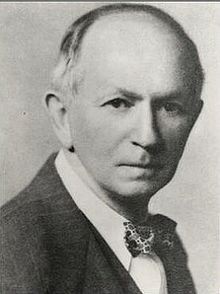
\includegraphics[width=0.25\linewidth]{images/Lotka} \end{center}

Alfred J. Lotka (1880-1949) was born to French-speaking American parents in Lemberg (then part of the Habsburg empire, now Lviv, Ukraine). He studied in France, Germany and England, receiving a BSc in 1901 and a DSc in 1912 from Birmingham university. He moved to the US in 1902, and worked at the US Patent office, as an editor of Scientific American, and as a statistician at the Metropolitan Life Insturance Company in NYC. He wrote more than a hundred papers and five books, spanning a large range of topics. He's best known for the book \emph{Elements of Physical Biology}, his contributions to demography, and one of the first studies dealing with bibliometrics \citep{lotka1926frequency}.

Starting in 1910 (reprinted as \citet{lotka2002contribution}) he investigated coupled differential equations relating to chemical as well as ecological dynamics. In \citet{lotka1920analytical} he studied a system of two ODEs that gave rise to perpetual oscillations: ``It was, therefore, with considerable surprise that the writer, on applying his method to certain special cases, found these to lead to undamped, and hence indefinitely continued, oscillations.'' He went on to describe ``1. A species of organism \(S_1\), a plant species, say, deriving its nourishment from a source presented in such large excess that the mass of the source may be considered constant during the period of time with which we are concerned. 2. A species \(S_2\), for example a herbivorous animal species, feeding on \(S_1\).''

The equations he derived (and then studied later in more detail) are now termed Lotka-Volterra equations.

\begin{center}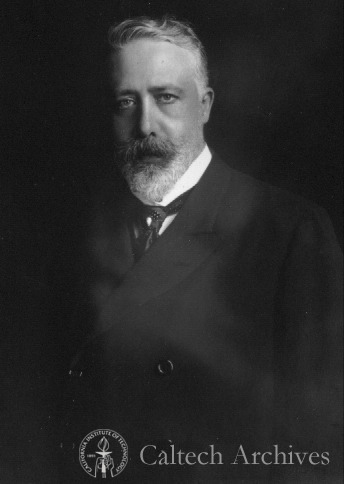
\includegraphics[width=0.25\linewidth]{images/Volterra} \end{center}

Vito Volterra (1860-1940) was born in Ancona (then part of the Papal State) in a poor jewish family. The financial situation precipitated with the death of his father, when Vito was two. Vito and his mother went to live with relatives in Turin and then Florence. Volterra showed amazing mathematical talent at a very early age. Antonio Roiti, professor of physics in Florence, noticed the budding mathematician and hired him as his assistant, so that he could continue his studies. He went on to enroll at the Scuola Normale in Pisa, receiving a degree in Physics in 1882. At age 23 he was made full professor of Rational Mechanics in Pisa, and then in 1900 of Mathematical Physics in Rome. For thirty years, he contributed important studies in mathematics, and enriched academic life in Italy (for example, he was the first director of the National Center for Research). In 1931 he refused to take an oath of loyalty to the fascist regime (only 12 professors out of 1250 refused), and was therefore forced to resign (his take on the fascist enterprise: ``Empires die, but Euclid's theorems keep their youth forever'').

His interest in mathematical ecology is due to Umberto d'Ancona (his son-in-law), who had studied the trends in fisheries in the Adriatic sea before and immediately after WWI. In 1914-1918 fisheries in the Adriatic had stopped completely because of the conflict. D'Ancona had noticed that, while herbivorous fish had remained about constant, the piscivorous fish had increased dramatically in numbers. The problem piqued Volterra who immediately published a sophisticated study, proposing the same equations studied by Lotka. In a short letter to Nature \citep{volterra1926fluctuations}, he stated the so-called ``Volterra's Effect'' (which he termed ``Law III''): ``a complete closure of the fishery was a form of `protection' under which the voracious fishes were much the better and prospered accordingly, but the ordinary food-fishes, on which these are accustomed to prey, were worse off than before.'' This brief paper was a summary of the much larger \citet{volterra1926variazioni}.

\hypertarget{lotka-volterra-interactions}{%
\subsection{Lotka-Volterra interactions}\label{lotka-volterra-interactions}}

In 1927, Lotka wrote to Nature to raise the issue that the equations studied by Volterra and the figures presented in Volterra's brief article were identical to those found in \emph{Elements of Physical Biology} (published in 1925). He concludes that ``It would be gratifying if Prof.~Volterra's publication should direct attention to a field and method of inquiry which apparently has hitherto passed almost unnoticed.''

Volterra graciously conceded ``I recognize his priority, and am sorry not to have known his work, and therefore not have been able to mention it.'' He however listed a few points in which the two authors had pursued different directions, and concluded ``Working independently the one from the other, we have found some common results, and this confirms the exactitude and the interest in the position of the problem. I agree with him in his conclusions that these studies and these methods of research deserve to receive greated attention from scholars, and should give rise to important applications.''

\hypertarget{basic-formulation}{%
\section{Basic formulation}\label{basic-formulation}}

We can write the Generalized Lotka-Volterra model in a compact form as:

\[
\dfrac{dx(t)}{dt} = D(x(t))(r + A x(t))
\]

where \(x(t)\) is a (column) vector of length \(n\) containing the densities of all populations \(1, \ldots, n\) at time \(t\), \(r\) is a vector of ``intrinsic growth rates'' (or death rates, when negative), measuring the growth (decline) of population \(i\) when grown alone at low density, and \(A\) is a \(n \times n\) matrix of interaction coefficients. We use \(D(x)\) to denote the diagonal matrix with \(x\) on the diagonal.

\hypertarget{a-single-population}{%
\section{A single population}\label{a-single-population}}

The simplest case to study is that of a single population, in which case the equation becomes that of the logistic growth:

\[
\dfrac{dx(t)}{dt} = x(t)(r + a x(t))
\]

This is a separable ODE, with solution:

\[
x(t) = \frac{r}{e^{-r \left(k+t\right)}-a}
\]
where \(k\) is a constant. Setting \(x(0) = x_0\) (i.e., providing an initial condition), solving for the constant and substituting:

\[
x(t) = \frac{r {x_0} e^{r t}}{r-a {x_0} \left(e^{r t}-1\right)}
\]
As such, provided with the parameters \(r\) and \(a\), as well as an initial condition, we can determine the population size for any time \(t\). For example, in \texttt{R}:

\begin{Shaded}
\begin{Highlighting}[]
\KeywordTok{library}\NormalTok{(deSolve) }\CommentTok{# integrate ODEs}
\KeywordTok{library}\NormalTok{(tidyverse) }\CommentTok{# plotting and wrangling}
\CommentTok{# define the differential equation}
\NormalTok{logistic_growth <-}\StringTok{ }\ControlFlowTok{function}\NormalTok{(t, x, parameters)\{}
  \KeywordTok{with}\NormalTok{(}\KeywordTok{as.list}\NormalTok{(}\KeywordTok{c}\NormalTok{(x, parameters)), \{}
\NormalTok{    dxdt <-}\StringTok{ }\NormalTok{x }\OperatorTok{*}\StringTok{ }\NormalTok{(r }\OperatorTok{+}\StringTok{ }\NormalTok{a }\OperatorTok{*}\StringTok{ }\NormalTok{x)}
    \KeywordTok{list}\NormalTok{(dxdt)}
\NormalTok{  \})}
\NormalTok{\}}
\CommentTok{# define parameters, integration time, initial conditions}
\NormalTok{times <-}\StringTok{ }\KeywordTok{seq}\NormalTok{(}\DecValTok{0}\NormalTok{, }\DecValTok{100}\NormalTok{, }\DataTypeTok{by =} \DecValTok{5}\NormalTok{)}
\NormalTok{x0 <-}\StringTok{ }\FloatTok{0.05}
\NormalTok{r <-}\StringTok{ }\FloatTok{0.1}
\NormalTok{a <-}\StringTok{ }\FloatTok{-0.05}
\NormalTok{parameters <-}\StringTok{ }\KeywordTok{list}\NormalTok{(}\DataTypeTok{r =}\NormalTok{ r, }\DataTypeTok{a =}\NormalTok{ a)}
\CommentTok{# solve numerically}
\NormalTok{out <-}\StringTok{ }\KeywordTok{ode}\NormalTok{(}\DataTypeTok{y =}\NormalTok{ x0, }\DataTypeTok{times =}\NormalTok{ times, }
           \DataTypeTok{func =}\NormalTok{ logistic_growth, }\DataTypeTok{parms =}\NormalTok{ parameters, }
           \DataTypeTok{method =} \StringTok{"ode45"}\NormalTok{)}
\CommentTok{# now compute analytically}
\NormalTok{solution <-}\StringTok{ }\NormalTok{r }\OperatorTok{*}\StringTok{ }\NormalTok{x0 }\OperatorTok{*}\StringTok{ }\KeywordTok{exp}\NormalTok{(r }\OperatorTok{*}\StringTok{ }\NormalTok{times) }\OperatorTok{/}\StringTok{ }\NormalTok{(r }\OperatorTok{-}\StringTok{ }\NormalTok{a }\OperatorTok{*}\StringTok{ }\NormalTok{x0 }\OperatorTok{*}\StringTok{ }\NormalTok{(}\KeywordTok{exp}\NormalTok{(r }\OperatorTok{*}\StringTok{ }\NormalTok{times) }\OperatorTok{-}\StringTok{ }\DecValTok{1}\NormalTok{))}
\CommentTok{# use ggplot to plot}
\NormalTok{res <-}\StringTok{ }\KeywordTok{tibble}\NormalTok{(}\DataTypeTok{time =}\NormalTok{ out[,}\DecValTok{1}\NormalTok{], }\DataTypeTok{x_t =}\NormalTok{ out[,}\DecValTok{2}\NormalTok{], }\DataTypeTok{x_sol =}\NormalTok{ solution)}
\KeywordTok{ggplot}\NormalTok{(}\DataTypeTok{data =}\NormalTok{ res) }\OperatorTok{+}\StringTok{ }\KeywordTok{aes}\NormalTok{(}\DataTypeTok{x =}\NormalTok{ time, }\DataTypeTok{y =}\NormalTok{ x_t) }\OperatorTok{+}\StringTok{ }
\StringTok{  }\KeywordTok{geom_line}\NormalTok{() }\OperatorTok{+}\StringTok{ }
\StringTok{  }\KeywordTok{geom_point}\NormalTok{(}\KeywordTok{aes}\NormalTok{(}\DataTypeTok{x =}\NormalTok{ time, }\DataTypeTok{y =}\NormalTok{ x_sol), }\DataTypeTok{colour =} \StringTok{"red"}\NormalTok{, }\DataTypeTok{shape =} \DecValTok{2}\NormalTok{) }\OperatorTok{+}\StringTok{ }
\StringTok{  }\KeywordTok{ylab}\NormalTok{(}\KeywordTok{expression}\NormalTok{(}\StringTok{"x(t)"}\NormalTok{)) }\OperatorTok{+}\StringTok{ }\KeywordTok{xlab}\NormalTok{(}\KeywordTok{expression}\NormalTok{(}\StringTok{"t"}\NormalTok{))}
\end{Highlighting}
\end{Shaded}

\begin{center}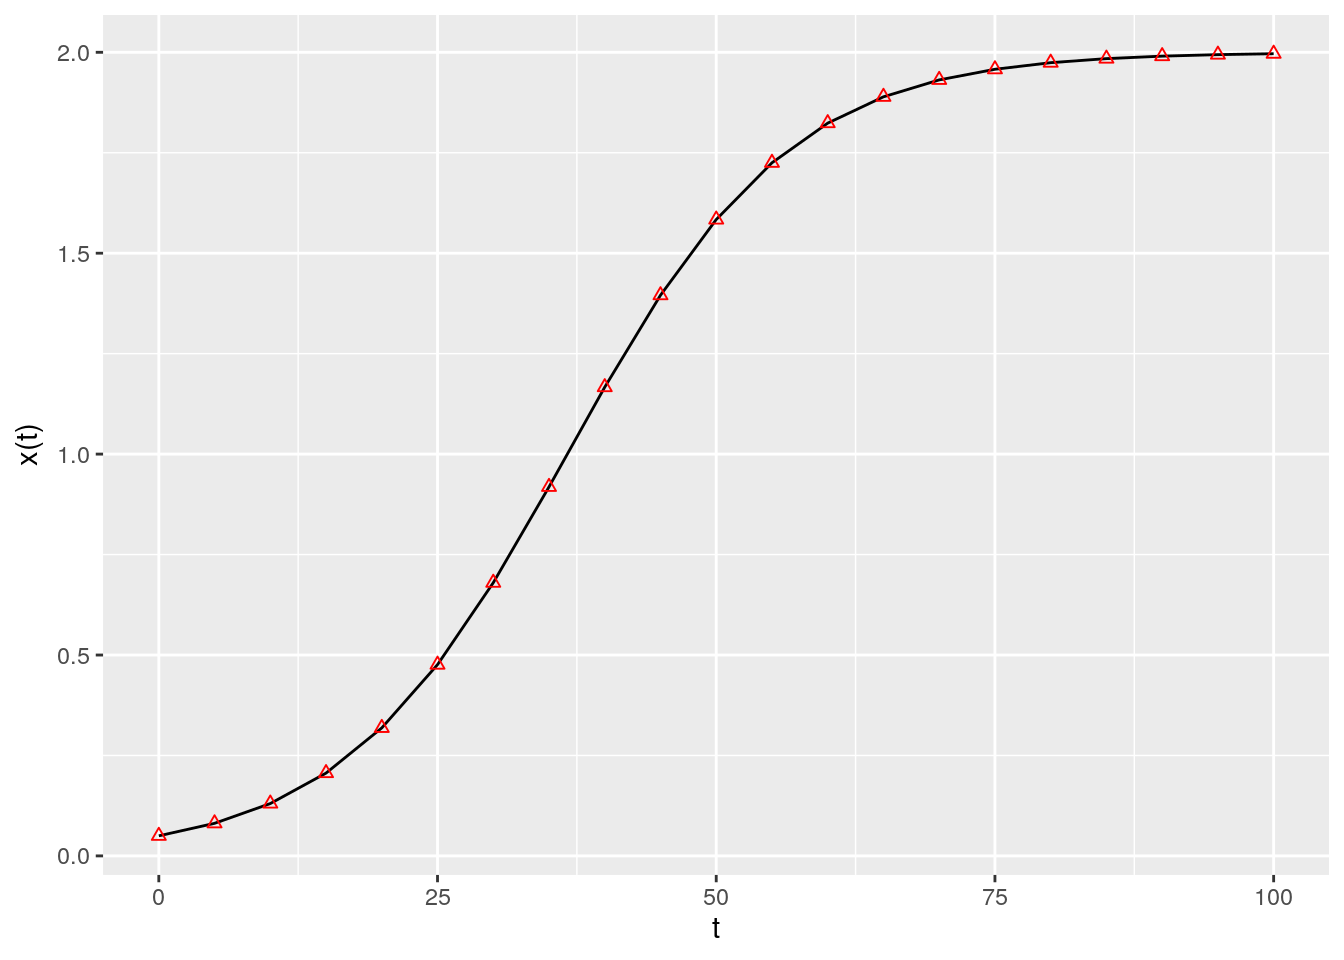
\includegraphics{A-Tour-of-the-Generalized-Lotka-Volterra-Model_files/figure-latex/logistic-1} \end{center}

If \(a < 0\) and \(r > 0\), the population started at any positive value eventually reaches an equilibrium, which we can find by setting \(dx(t)/dt = 0\) and considering \(x \neq 0\):

\[
(r + a x) = 0 \to x = -\frac{r}{a}
\]

\hypertarget{metapopulation-dynamics}{%
\subsection{Metapopulation dynamics}\label{metapopulation-dynamics}}

Consider a fragmented landscape in which habitable patches are connected by dispersal (for simplicity, suppose that all patches are reachable from any other). Call \(p(t)\) the proportion of patches occupied by the species of interest at time \(t\), and assume that a) an empty patch (the proportion of empty patches is \(1 - p(t)\)) is colonized by the species with rate \(c p(t)\), where \(c\) is the ``colonization rate'', and b) that occupied patches become empty at rate \(e p(t)\) (``extinction rate''). We want to model the proportion of patches occupied by the population at time \(t\):

\[
\dfrac{d p(t)}{dt} = c p(t)(1 - p(t)) - e p(t) = p(t) (c - (c + e) p(t))
\]

which is equivalent to the logistic equation above with \(r = c\) and \(a = -(c+e)\). As such, asymptotically the proportion of patches occupied by the population will be \(-r/a = c / (c + e)\).

\hypertarget{s-i-s-model}{%
\subsection{S-I-S model}\label{s-i-s-model}}

Consider a population of individuals, each of which can be in one of two states: susceptible to a disease, or infective/infected. Call \(S(t)\) the proportion of susceptible individuals at time \(t\), and \(I(t)\) the proportion of infected individuals, with \(S(t) + I(t) = 1\). When individuals meet, an infected individual can transmit the disease to susceptibles with rate \(\beta\); infected individuals recover from the disease with rate \(\gamma\), and return susceptible. We can write the system of equations:

\[
\begin{cases}
\dfrac{d S(t)}{dt} = -\beta S(t) I(t) + \gamma I(t)\\
\dfrac{d I(t)}{dt} = \beta S(t) I(t) - \gamma I(t)
\end{cases}
\]

take the second equation, and substitute \(S(t) = 1 - I(t)\); rearranging:

\[
\dfrac{d I(t)}{dt} = \beta (1-I(t)) I(t) - \gamma I(t) = I(t)(\beta - \gamma -\beta I(t))
\]

which is again the equation for the logistic growth with \(r = \beta - \gamma\) and \(a = -\beta\). As such, provided that \(\beta -\gamma > 0\), asymptotically a fraction \((\beta - \gamma) / \beta\) of individuals will be infected. The condition \(\beta -\gamma > 0 \to \beta > \gamma \to \beta/ \gamma > 1\) is often written as \(\mathcal R_0 = \beta/ \gamma > 1\).

\hypertarget{multi-species-dynamics}{%
\section{Multi-species dynamics}\label{multi-species-dynamics}}

\hypertarget{existence-of-an-equilibrium}{%
\subsection{Existence of an equilibrium}\label{existence-of-an-equilibrium}}

Returning to the multi-species system, and in analogy with the single species, we can look for stationary points (equilibria). If the matrix \(A\) is not singular, then we can look for a solution of \(r + Ax\) that has positive components (called a \textbf{feasible equilibrium}). \textbf{If such point exists, it is unique} and is the solution of \(Ax^\star = -r\), \(x^\star = -A^{-1}r\).

Suppose that the GLV has no feasible equilibrium. Then all trajectories (if bounded; some could grow to infinity) reach the boundary of \(\mathbb R^n_{0+}\). Practically, this means that \textbf{to ensure coexistence of all species, it is necessary to have an equilibrium in the interior \(\mathbb R^n_{+}\)}.

\hypertarget{stability-of-an-equilibrium}{%
\subsection{Stability of an equilibrium}\label{stability-of-an-equilibrium}}

Suppose that a feasible equilibrium \(x^\star\) exists. Then we can ask whether it is \textbf{attractive}, i.e.~if trajectories started at initial condition \(x(0)\) will eventually reach \(x^\star\). This problem is in general difficult to solve (but see below); as an alternative we can test for \textbf{local asymptotic stability}, i.e., ask whether \textbf{the system will return to the equilibrium if perturbed infinitesimally away from it}. In general, whenever we describe an ecological community as a system of nonlinear, autonomous ODEs:

\[
\frac{d x_i (t)}{d t} = f_i (x(t)) \;,
\]
we define an equilibrium \(x^\star\) as a vector of densities such that:

\[
\left. \frac{d x_i}{d t} \right|_{{x}^\star} = f_i
({x}^\star) = 0 \quad \forall i
\]
A given system might have a multitude of equilibria. When the system is resting at an equilibrium point, it will remain there unless it is perturbed away from it. Local stability analysis is a method to probe whether a system that is perturbed infinitesimally away from an equilibrium will eventually return to it, or rather move away from it.

Suppose that the system is resting at an equilibrium \(x^\star\), and that it is slightly perturbed away from it. \(\Delta x(0) = x(0)-x^\star\) is the state of the system immediately after the perturbation. We Taylor-expand around \(x^\star\):

\[
f(\Delta x(0)) = f(x^\star)+ \left. J \right|_{x^\star} \Delta x(0) + \ldots
\]

Where \(J\) is the Jacobian matrix of the system, whose elements are defined as:

\[
J_{ij} = \frac{\partial f_i({x})}{\partial x_j} 
\]

Each element of this matrix is therefore a function, whose value depends on \({x}\). When we evaluate the Jacobian matrix at an equilibrium point \({x}^\star\), we obtain the so-called ``community matrix'' \({M}\):

\[
  M = \left. {J} \right|_{ {x}^\star}
\]

Note that, although each system has a unique Jacobian matrix, there are as many community matrices as there are equilibria. The community matrix details the effect of increasing the density of one species on any other species around the equilibrium point.

We can therefore write the differential equation:

\[
\frac{d \Delta x(t)}{dt} \approx M \Delta x(t)
\]
with solution:

\[
\Delta x(t) = \Delta x(0) e^{Mt} = \Delta x(0) L e^{\Lambda t} R
\]

Where \(L\) and \(R\) are matrices containing the left and right eigenvectors of \(M\), and \(\Lambda\) is a diagonal matrix containing the eigenvalues of \(M\). As such, the eigenvalues of \(M\) determine the stability of the equilibrium \({x}^\star\): if all the eigenvalues have negative real part, then the system will eventually return to the equilibrium after sufficiently small perturbations; conversely, if any of the eigenvalues have positive real part, the system will move away from the equilibrium whenever perturbed. Therefore, depending on the sign of the ``rightmost'' eigenvalue of \({M}\), \(\lambda_1\), we can determine the stability of \({x}^\star\):

\[
  \text{Re}(\lambda_1) \begin{cases}
    < 0 \to {x}^\star \quad \text{is stable}\\
    > 0 \to {x}^\star \quad \text{is unstable}
  \end{cases}
\]

Local asymptotic stability means that the equilibrium is stable with respect to infinitesimal perturbations (``local''), and that returning to the equilibrium could take a long time (``asymptotic''). Ecologists have also studied stronger forms of stability (e.g., ``global stability'', in which all trajectories started at positive densities lead to the equilibrium).

For the GLV model, the Jacobian is easy to compute:

\[
J_{ij} = \frac{\partial f_i}{\partial x_j} = a_{ij} x_i
\]

and

\[
J_{ii} = \frac{\partial f_i}{\partial x_i} = r_i + \sum_j a_{ij} x_j + a_{ii} x_i
\]

At equilibrium \(r_i + \sum_j a_{ij} x_j = 0\), and therefore:

\[
M = \left. {J} \right|_{ {x}^\star} = D(x^\star)A
\]

\hypertarget{types-of-dynamics}{%
\section{Types of dynamics}\label{types-of-dynamics}}

For a single population, there are only three types of dynamics that can be displayed by a GLV model: either the population grows to infinity, shrinks to zero, or asymptotically reaches a steady state.

\citet{smale1976differential} and \citet{hirsch1982systems} showed that limit cylces are possible for three or more species, and that any dynamics can be found for competitive GLV systems with five or more species.

The code necessary for some numerical explorations:

\begin{Shaded}
\begin{Highlighting}[]
\CommentTok{# Generalized Lotka-Volterra model}
\NormalTok{GLV <-}\StringTok{ }\ControlFlowTok{function}\NormalTok{(t, x, parameters)\{}
  \KeywordTok{with}\NormalTok{(}\KeywordTok{as.list}\NormalTok{(}\KeywordTok{c}\NormalTok{(x, parameters)), \{}
\NormalTok{    x[x }\OperatorTok{<}\StringTok{ }\DecValTok{10}\OperatorTok{^-}\DecValTok{8}\NormalTok{] <-}\StringTok{ }\DecValTok{0} \CommentTok{# prevent numerical problems}
\NormalTok{    dxdt <-}\StringTok{ }\NormalTok{x }\OperatorTok{*}\StringTok{ }\NormalTok{(r }\OperatorTok{+}\StringTok{ }\NormalTok{A }\OperatorTok\StringTok{ }\NormalTok{x)}
    \KeywordTok{list}\NormalTok{(dxdt)}
\NormalTok{  \})}
\NormalTok{\}}
\CommentTok{# function to plot output}
\NormalTok{plot_ODE_output <-}\StringTok{ }\ControlFlowTok{function}\NormalTok{(out)\{}
\NormalTok{  out <-}\StringTok{ }\KeywordTok{as.data.frame}\NormalTok{(out)}
  \KeywordTok{colnames}\NormalTok{(out) <-}\StringTok{ }\KeywordTok{c}\NormalTok{(}\StringTok{"time"}\NormalTok{, }\KeywordTok{paste}\NormalTok{(}\StringTok{"sp"}\NormalTok{, }\DecValTok{1}\OperatorTok{:}\NormalTok{(}\KeywordTok{ncol}\NormalTok{(out) }\DecValTok{-1}\NormalTok{), }\DataTypeTok{sep =} \StringTok{"_"}\NormalTok{))}
\NormalTok{  out <-}\StringTok{ }\KeywordTok{as_tibble}\NormalTok{(out) }\OperatorTok\StringTok{ }\KeywordTok{gather}\NormalTok{(species, density, }\OperatorTok{-}\NormalTok{time)}
\NormalTok{  pl <-}\StringTok{ }\KeywordTok{ggplot}\NormalTok{(}\DataTypeTok{data =}\NormalTok{ out) }\OperatorTok{+}\StringTok{ }
\StringTok{    }\KeywordTok{aes}\NormalTok{(}\DataTypeTok{x =}\NormalTok{ time, }\DataTypeTok{y =}\NormalTok{ density, }\DataTypeTok{colour =}\NormalTok{ species) }\OperatorTok{+}\StringTok{ }
\StringTok{    }\KeywordTok{geom_line}\NormalTok{()}
  \KeywordTok{show}\NormalTok{(pl)}
  \KeywordTok{return}\NormalTok{(out)}
\NormalTok{\}}
\CommentTok{# general function to integrate GLV}
\NormalTok{integrate_GLV <-}\StringTok{ }\ControlFlowTok{function}\NormalTok{(r, A, x0, }\DataTypeTok{maxtime =} \DecValTok{100}\NormalTok{, }\DataTypeTok{steptime =} \FloatTok{0.5}\NormalTok{)\{}
\NormalTok{  times <-}\StringTok{ }\KeywordTok{seq}\NormalTok{(}\DecValTok{0}\NormalTok{, maxtime, }\DataTypeTok{by =}\NormalTok{ steptime)}
\NormalTok{  parameters <-}\StringTok{ }\KeywordTok{list}\NormalTok{(}\DataTypeTok{r =}\NormalTok{ r, }\DataTypeTok{A =}\NormalTok{ A)}
  \CommentTok{# solve numerically}
\NormalTok{  out <-}\StringTok{ }\KeywordTok{ode}\NormalTok{(}\DataTypeTok{y =}\NormalTok{ x0, }\DataTypeTok{times =}\NormalTok{ times, }
           \DataTypeTok{func =}\NormalTok{ GLV, }\DataTypeTok{parms =}\NormalTok{ parameters, }
           \DataTypeTok{method =} \StringTok{"ode45"}\NormalTok{)}
  \CommentTok{# plot and make into tidy form}
\NormalTok{  out <-}\StringTok{ }\KeywordTok{plot_ODE_output}\NormalTok{(out)}
  \KeywordTok{return}\NormalTok{(out)}
\NormalTok{\}}
\end{Highlighting}
\end{Shaded}

A few examples taken from \citet{barabas2016effect}. First, a competitive system in which a feasible equilibrium does not exist, leading to the extinction of a species:

\begin{Shaded}
\begin{Highlighting}[]
\KeywordTok{set.seed}\NormalTok{(}\DecValTok{1}\NormalTok{) }\CommentTok{# for reproducibility}
\NormalTok{r_}\DecValTok{1}\NormalTok{ <-}\StringTok{ }\KeywordTok{rep}\NormalTok{(}\DecValTok{1}\NormalTok{, }\DecValTok{3}\NormalTok{)}
\NormalTok{A_}\DecValTok{1}\NormalTok{ <-}\StringTok{ }\OperatorTok{-}\KeywordTok{matrix}\NormalTok{(}\KeywordTok{c}\NormalTok{(}\DecValTok{10}\NormalTok{, }\DecValTok{9}\NormalTok{, }\DecValTok{5}\NormalTok{, }
                 \DecValTok{9}\NormalTok{, }\DecValTok{10}\NormalTok{, }\DecValTok{9}\NormalTok{, }
                 \DecValTok{5}\NormalTok{, }\DecValTok{9}\NormalTok{, }\DecValTok{10}\NormalTok{), }\DecValTok{3}\NormalTok{, }\DecValTok{3}\NormalTok{, }\DataTypeTok{byrow =} \OtherTok{TRUE}\NormalTok{)}
\CommentTok{# check the existence of feasible equilibrium}
\KeywordTok{print}\NormalTok{(}\KeywordTok{solve}\NormalTok{(A_}\DecValTok{1}\NormalTok{, }\OperatorTok{-}\NormalTok{r_}\DecValTok{1}\NormalTok{)) }\CommentTok{# not feasible}
\NormalTok{x0_}\DecValTok{1}\NormalTok{ <-}\StringTok{ }\KeywordTok{runif}\NormalTok{(}\DecValTok{3}\NormalTok{)}
\NormalTok{res_}\DecValTok{1}\NormalTok{ <-}\StringTok{ }\KeywordTok{integrate_GLV}\NormalTok{(r_}\DecValTok{1}\NormalTok{, A_}\DecValTok{1}\NormalTok{, x0_}\DecValTok{1}\NormalTok{)}
\end{Highlighting}
\end{Shaded}

\begin{center}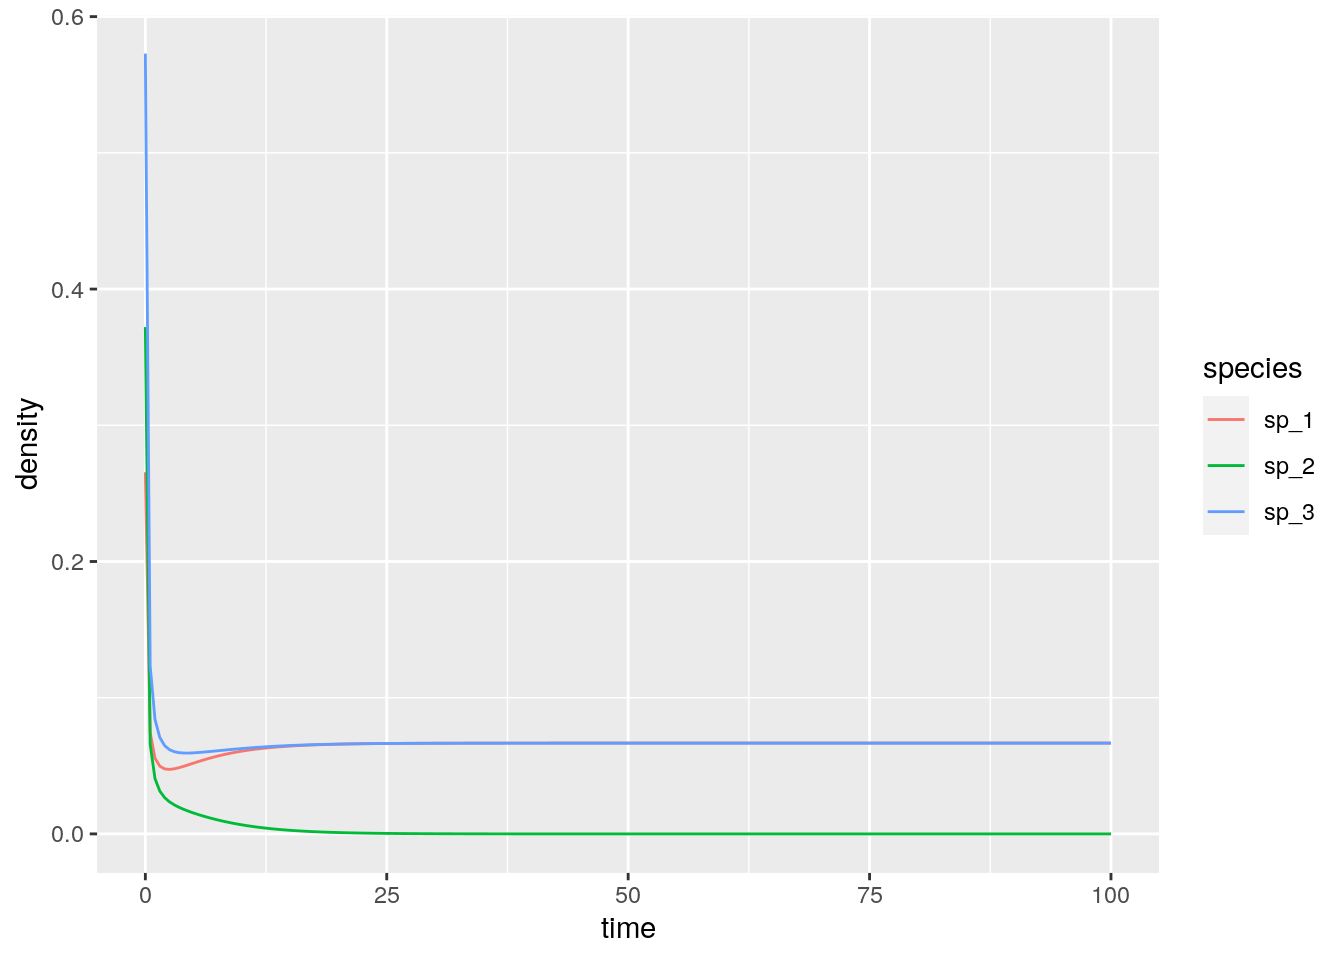
\includegraphics{A-Tour-of-the-Generalized-Lotka-Volterra-Model_files/figure-latex/glvex1-1} \end{center}

\begin{verbatim}
# [1] -0.08333333  0.25000000 -0.08333333
\end{verbatim}

Then, a case in which the equilibrium exists, and is attractive (stable):

\begin{Shaded}
\begin{Highlighting}[]
\KeywordTok{set.seed}\NormalTok{(}\DecValTok{2}\NormalTok{) }\CommentTok{# for reproducibility}
\NormalTok{r_}\DecValTok{2}\NormalTok{ <-}\StringTok{ }\KeywordTok{rep}\NormalTok{(}\DecValTok{10}\NormalTok{, }\DecValTok{3}\NormalTok{)}
\NormalTok{A_}\DecValTok{2}\NormalTok{ <-}\StringTok{ }\OperatorTok{-}\KeywordTok{matrix}\NormalTok{(}\KeywordTok{c}\NormalTok{(}\DecValTok{10}\NormalTok{, }\DecValTok{7}\NormalTok{, }\DecValTok{12}\NormalTok{, }
                 \DecValTok{15}\NormalTok{, }\DecValTok{10}\NormalTok{, }\DecValTok{8}\NormalTok{, }
                 \DecValTok{7}\NormalTok{, }\DecValTok{11}\NormalTok{, }\DecValTok{10}\NormalTok{), }\DecValTok{3}\NormalTok{, }\DecValTok{3}\NormalTok{, }\DataTypeTok{byrow =} \OtherTok{TRUE}\NormalTok{)}
\CommentTok{# check the existence of feasible equilibrium}
\KeywordTok{print}\NormalTok{(}\KeywordTok{solve}\NormalTok{(A_}\DecValTok{2}\NormalTok{, }\OperatorTok{-}\NormalTok{r_}\DecValTok{2}\NormalTok{)) }\CommentTok{# feasible}
\NormalTok{x0_}\DecValTok{2}\NormalTok{ <-}\StringTok{ }\KeywordTok{runif}\NormalTok{(}\DecValTok{3}\NormalTok{)}
\NormalTok{res_}\DecValTok{2}\NormalTok{ <-}\StringTok{ }\KeywordTok{integrate_GLV}\NormalTok{(r_}\DecValTok{2}\NormalTok{, A_}\DecValTok{2}\NormalTok{, x0_}\DecValTok{2}\NormalTok{)}
\end{Highlighting}
\end{Shaded}

\begin{center}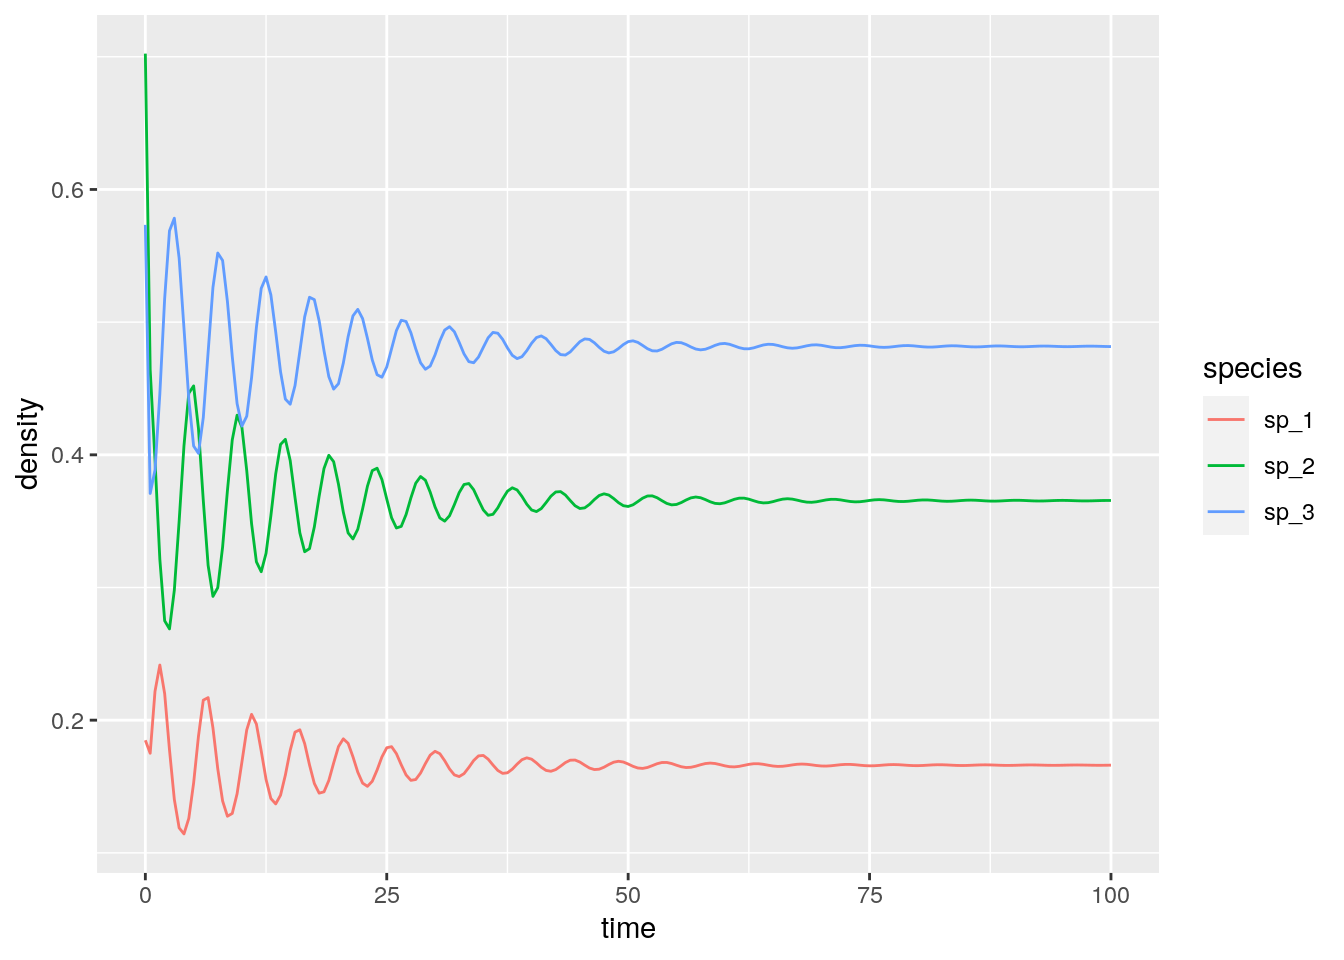
\includegraphics{A-Tour-of-the-Generalized-Lotka-Volterra-Model_files/figure-latex/glvex2-1} \end{center}

\begin{verbatim}
# [1] 0.1661130 0.3654485 0.4817276
\end{verbatim}

With three competitors we can find stable limit cycles:

\begin{Shaded}
\begin{Highlighting}[]
\KeywordTok{set.seed}\NormalTok{(}\DecValTok{3}\NormalTok{) }\CommentTok{# for reproducibility}
\NormalTok{r_}\DecValTok{3}\NormalTok{ <-}\StringTok{ }\KeywordTok{rep}\NormalTok{(}\DecValTok{1}\NormalTok{, }\DecValTok{3}\NormalTok{)}
\NormalTok{A_}\DecValTok{3}\NormalTok{ <-}\StringTok{ }\OperatorTok{-}\KeywordTok{matrix}\NormalTok{(}\KeywordTok{c}\NormalTok{(}\DecValTok{10}\NormalTok{, }\DecValTok{6}\NormalTok{, }\DecValTok{12}\NormalTok{, }
                 \DecValTok{14}\NormalTok{, }\DecValTok{10}\NormalTok{, }\DecValTok{2}\NormalTok{, }
                 \DecValTok{8}\NormalTok{, }\DecValTok{18}\NormalTok{, }\DecValTok{10}\NormalTok{), }\DecValTok{3}\NormalTok{, }\DecValTok{3}\NormalTok{, }\DataTypeTok{byrow =} \OtherTok{TRUE}\NormalTok{)}
\CommentTok{# check the existence of feasible equilibrium}
\KeywordTok{print}\NormalTok{(}\KeywordTok{solve}\NormalTok{(A_}\DecValTok{3}\NormalTok{, }\OperatorTok{-}\NormalTok{r_}\DecValTok{3}\NormalTok{)) }\CommentTok{# feasible}
\NormalTok{x0_}\DecValTok{3}\NormalTok{ <-}\StringTok{ }\FloatTok{0.1} \OperatorTok{*}\StringTok{ }\KeywordTok{runif}\NormalTok{(}\DecValTok{3}\NormalTok{)}
\NormalTok{res_}\DecValTok{3}\NormalTok{ <-}\StringTok{ }\KeywordTok{integrate_GLV}\NormalTok{(r_}\DecValTok{3}\NormalTok{, A_}\DecValTok{3}\NormalTok{, x0_}\DecValTok{3}\NormalTok{, }\DataTypeTok{maxtime =} \DecValTok{250}\NormalTok{)}
\end{Highlighting}
\end{Shaded}

\begin{center}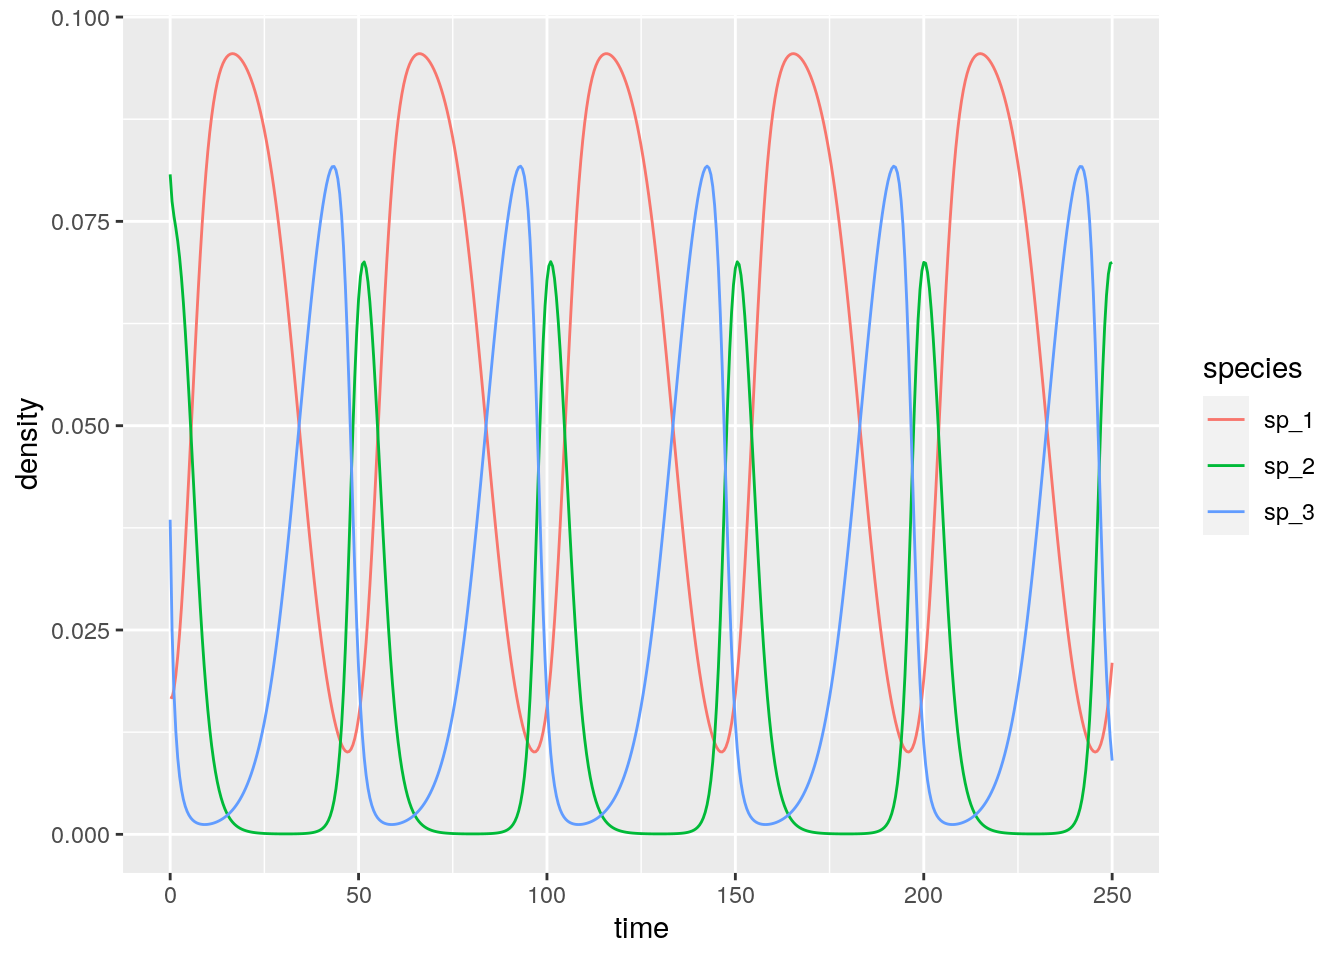
\includegraphics{A-Tour-of-the-Generalized-Lotka-Volterra-Model_files/figure-latex/glvex3-1} \end{center}

\begin{verbatim}
# [1] 0.05714286 0.01428571 0.02857143
\end{verbatim}

And with four or more species we can have chaos:

\begin{Shaded}
\begin{Highlighting}[]
\KeywordTok{set.seed}\NormalTok{(}\DecValTok{4}\NormalTok{) }\CommentTok{# for reproducibility}
\NormalTok{r_}\DecValTok{4}\NormalTok{ <-}\StringTok{ }\KeywordTok{c}\NormalTok{(}\DecValTok{1}\NormalTok{, }\FloatTok{0.72}\NormalTok{, }\FloatTok{1.53}\NormalTok{, }\FloatTok{1.27}\NormalTok{)}
\NormalTok{A_}\DecValTok{4}\NormalTok{ <-}\StringTok{ }\OperatorTok{-}\KeywordTok{matrix}\NormalTok{(}\KeywordTok{c}\NormalTok{(}\DecValTok{1}\NormalTok{, }\FloatTok{1.09}\NormalTok{, }\FloatTok{1.52}\NormalTok{, }\DecValTok{0}\NormalTok{, }
                 \DecValTok{0}\NormalTok{, }\FloatTok{0.72}\NormalTok{, }\FloatTok{0.3168}\NormalTok{, }\FloatTok{0.9792}\NormalTok{, }
                 \FloatTok{3.5649}\NormalTok{, }\DecValTok{0}\NormalTok{, }\FloatTok{1.53}\NormalTok{, }\FloatTok{0.7191}\NormalTok{,}
                 \FloatTok{1.5367}\NormalTok{, }\FloatTok{0.6477}\NormalTok{, }\FloatTok{0.4445}\NormalTok{, }\FloatTok{1.27}\NormalTok{), }\DecValTok{4}\NormalTok{, }\DecValTok{4}\NormalTok{, }\DataTypeTok{byrow =} \OtherTok{TRUE}\NormalTok{)}
\CommentTok{# check the existence of feasible equilibrium}
\KeywordTok{print}\NormalTok{(}\KeywordTok{solve}\NormalTok{(A_}\DecValTok{4}\NormalTok{, }\OperatorTok{-}\NormalTok{r_}\DecValTok{4}\NormalTok{)) }\CommentTok{# feasible}
\NormalTok{x0_}\DecValTok{4}\NormalTok{ <-}\StringTok{ }\FloatTok{0.1} \OperatorTok{*}\StringTok{ }\KeywordTok{runif}\NormalTok{(}\DecValTok{4}\NormalTok{)}
\NormalTok{res_}\DecValTok{4}\NormalTok{ <-}\StringTok{ }\KeywordTok{integrate_GLV}\NormalTok{(r_}\DecValTok{4}\NormalTok{, A_}\DecValTok{4}\NormalTok{, x0_}\DecValTok{4}\NormalTok{, }\DataTypeTok{maxtime =} \DecValTok{500}\NormalTok{)}
\end{Highlighting}
\end{Shaded}

\begin{center}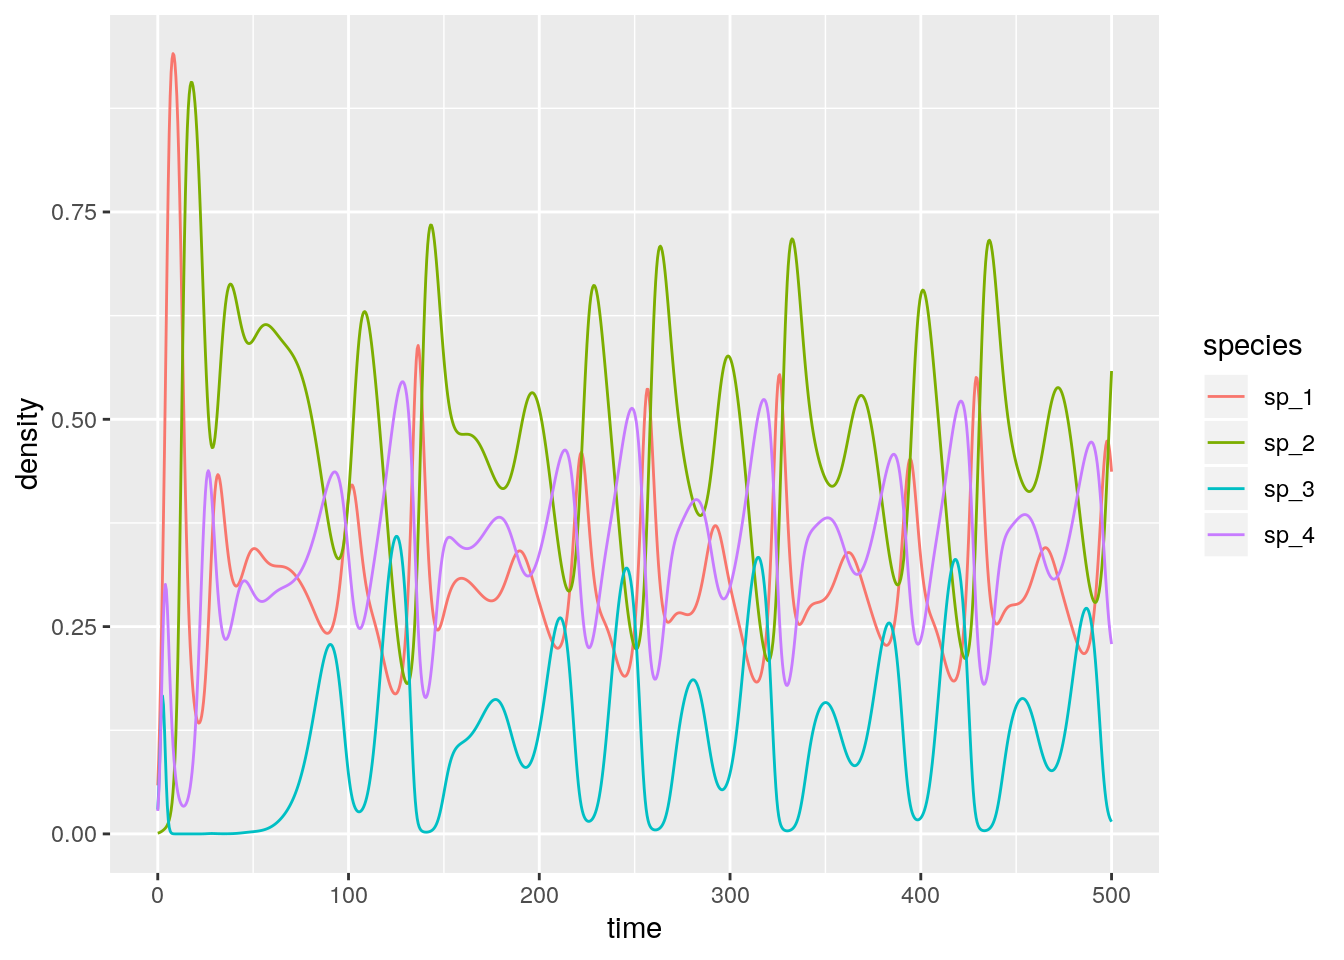
\includegraphics{A-Tour-of-the-Generalized-Lotka-Volterra-Model_files/figure-latex/glvex4-1} \end{center}

\begin{verbatim}
# [1] 0.3013030 0.4586546 0.1307655 0.3557416
\end{verbatim}

\hypertarget{the-equilibrium-is-the-time-average}{%
\section{The equilibrium is the time-average}\label{the-equilibrium-is-the-time-average}}

Suppose that \(x(t)\) has a periodic orbit of period \(T\). Further, assume that the GLV has an interior equilibrium \(x^\star\). We want to calculate the average density for each species:

\[
\frac{1}{T} \int_0^T x(t) dt
\]

We perform the change of variable \(y = \log(x(t))\), finding \(\frac{d x(t)}{dt} = \frac{d x(t)}{d \log(x(t))}\frac{d \log(x(t))}{dt} = x(t)\frac{d \log(x(t))}{dt}\). Then:

\[
\frac{d \log(x(t))}{dt} = r + Ax(t)
\]

Compute the average on both sides:

\[
\frac{1}{T}\int_0^T \frac{d \log(x(t))}{dt} dt= \frac{1}{T}\int_0^T \left(r + Ax \right) dt
\]

yielding:
\[
\frac{1}{T}(\log(x(T)) - \log(x(0))) = 0 = r + A \left( \frac{1}{T} \int_0^T x(t) dt \right)
\]
multiplying by the matrix inverse and rearranging:

\[
-A^{-1} r = x^\star =  \frac{1}{T} \int_0^T x(t) dt 
\]

showing that \textbf{the average density is} in fact \textbf{the equilibrium}. With a similar argument, one can prove that the trajectory stays in a compact space (i.e., in case of chaotic attractors), then long-time average is still \(x^\star\).

For example, let's compute the average for the system with the limit cycle above (discarding the transients in the first part of the time series):

\begin{Shaded}
\begin{Highlighting}[]
\NormalTok{res_}\DecValTok{3} \OperatorTok\StringTok{ }\KeywordTok{filter}\NormalTok{(time }\OperatorTok{>}\StringTok{ }\DecValTok{50}\NormalTok{) }\OperatorTok\StringTok{ }
\StringTok{  }\KeywordTok{group_by}\NormalTok{(species) }\OperatorTok\StringTok{ }
\StringTok{  }\KeywordTok{summarize}\NormalTok{(}\DataTypeTok{average =} \KeywordTok{mean}\NormalTok{(density))}
\CommentTok{# compare with equilibrium}
\KeywordTok{solve}\NormalTok{(A_}\DecValTok{3}\NormalTok{, }\OperatorTok{-}\NormalTok{r_}\DecValTok{3}\NormalTok{)}
\end{Highlighting}
\end{Shaded}

\begin{verbatim}
# # A tibble: 3 x 2
#   species average
#   <chr>     <dbl>
# 1 sp_1     0.0568
# 2 sp_2     0.0147
# 3 sp_3     0.0284
# [1] 0.05714286 0.01428571 0.02857143
\end{verbatim}

Repeat for the chaotic system:

\begin{Shaded}
\begin{Highlighting}[]
\NormalTok{res_}\DecValTok{4} \OperatorTok\StringTok{ }\KeywordTok{filter}\NormalTok{(time }\OperatorTok{>}\StringTok{ }\DecValTok{50}\NormalTok{) }\OperatorTok\StringTok{ }
\StringTok{  }\KeywordTok{group_by}\NormalTok{(species) }\OperatorTok\StringTok{ }
\StringTok{  }\KeywordTok{summarize}\NormalTok{(}\DataTypeTok{average =} \KeywordTok{mean}\NormalTok{(density))}
\CommentTok{# compare with equilibrium}
\KeywordTok{solve}\NormalTok{(A_}\DecValTok{4}\NormalTok{, }\OperatorTok{-}\NormalTok{r_}\DecValTok{4}\NormalTok{)}
\end{Highlighting}
\end{Shaded}

\begin{verbatim}
# # A tibble: 4 x 2
#   species average
#   <chr>     <dbl>
# 1 sp_1      0.303
# 2 sp_2      0.463
# 3 sp_3      0.126
# 4 sp_4      0.354
# [1] 0.3013030 0.4586546 0.1307655 0.3557416
\end{verbatim}

\hypertarget{d-stability-and-lyapunov-function}{%
\section{D-stability and Lyapunov function}\label{d-stability-and-lyapunov-function}}

Suppose that there is a positive diagonal matrix \(C\) such that \(CA + A^t C\) is negative definite (i.e., has only negative eigenvalues; the eigenvalues are real because the matrix is symmetric). Further, suppose that the GLV system with parameters \(A\) and \(r\) has a feasible equilibrium point \(x^\star\). Then the function:

\[
V(x(t)) = 1^t D(y) \left( x(t) -D(x^\star) \log x(t)\right)
\]
is a Lyapunov function for the GLV system.

To prove this point, we start from \(r = -Ax^\star\). Substituting, we can write the GLV system as \(dx(t)/dt = D(x)A(x - x^\star)\); similarly, we can write \(d \log x(t)/dt = A(x - x^\star)\). Taking the derivative of \(V\) with respect to time:

\[
\begin{aligned}
 \frac{d V(x(t))}{dt} &= 1^t C \left(\frac{d x(t)}{dt}  + D(x^*) \frac{d \log x(t)}{dt} \right)\\
 &= 1^t C \left(A (x - x^\star)  + D(x^*) A (x - x^\star) \right)\\
 &= 1^t C \left(D(x - x^\star)  A (x - x^\star) \right)\\
 &= 1^t \left(D(x - x^\star)  C A (x - x^\star) \right)\\
 &= (x - x^\star)^t  CA (x - x^\star)\\
 &= \frac{1}{2}(x - x^\star)^t  (CA + A^t C) (x - x^\star)\\
\end{aligned}
\]

A matrix \(B\) is negative definite if \(y^t B y < 0\) for all \(y \neq 0\). As such \(\frac{d V(x(t))}{dt} \leq 0\), i.e., will decrease in time (starting from any \(x(0)\)) until the equilibrium \(x^\star\) is reached.

Take a matrix \(A\) such that for a positive diagonal matrix \(C\), \(CA + A^tC\) is negative definite. Then \(A\) is said to be \textbf{D-stable}. The results above show that \textbf{if \(A\) is D-stable and a feasible equilibrium \(x^\star\) exists, than all trajectories starting at a positive density will converge to the equilibrium}. This property is often used to assess \textbf{global stability}.

A simple numerical example with two species:

\begin{Shaded}
\begin{Highlighting}[]
\NormalTok{r <-}\StringTok{ }\KeywordTok{c}\NormalTok{(}\DecValTok{1}\NormalTok{, }\DecValTok{1}\NormalTok{)}
\NormalTok{A <-}\StringTok{ }\KeywordTok{matrix}\NormalTok{(}\KeywordTok{c}\NormalTok{(}\OperatorTok{-}\DecValTok{1}\NormalTok{, }\DecValTok{3}\OperatorTok{/}\DecValTok{2}\NormalTok{, }\DecValTok{-1}\OperatorTok{/}\DecValTok{2}\NormalTok{, }\DecValTok{-1}\NormalTok{), }\DecValTok{2}\NormalTok{, }\DecValTok{2}\NormalTok{)}
\CommentTok{# the eigenvalues of A + A^t are -1 and -3, hence A is D-stable}
\KeywordTok{eigen}\NormalTok{(A }\OperatorTok{+}\StringTok{ }\KeywordTok{t}\NormalTok{(A))}\OperatorTok{$}\NormalTok{values}
\CommentTok{# now integrate from random initial condition---this should always }
\CommentTok{# converge to the equilibrium}
\KeywordTok{solve}\NormalTok{(A, }\OperatorTok{-}\NormalTok{r)}
\NormalTok{res <-}\StringTok{ }\KeywordTok{integrate_GLV}\NormalTok{(r, A, }\KeywordTok{abs}\NormalTok{(}\KeywordTok{rnorm}\NormalTok{(}\DecValTok{2}\NormalTok{)))}
\end{Highlighting}
\end{Shaded}

\begin{center}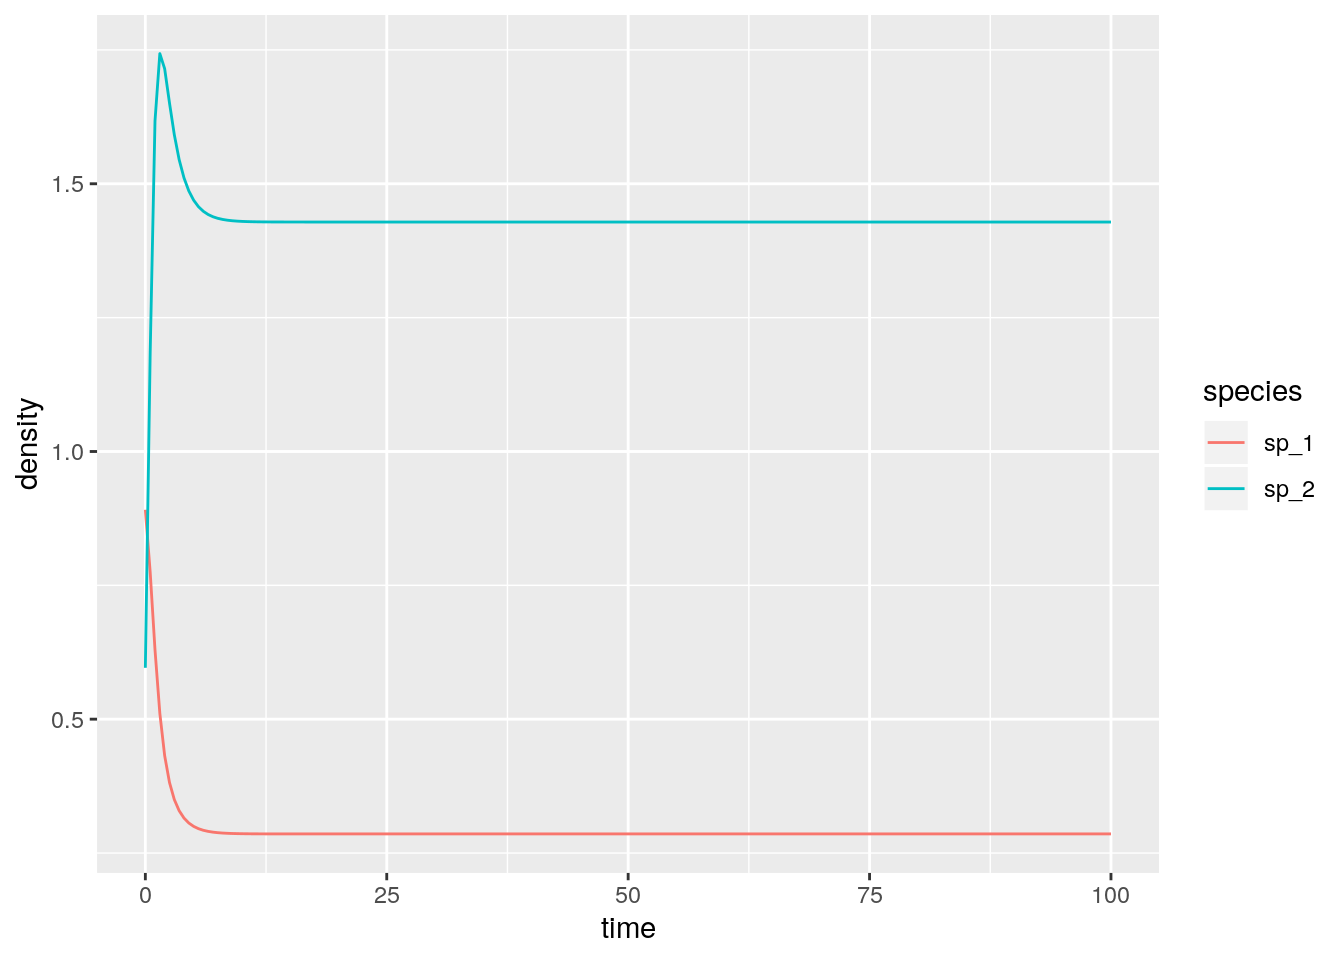
\includegraphics{A-Tour-of-the-Generalized-Lotka-Volterra-Model_files/figure-latex/globalst2-1} \end{center}

\begin{Shaded}
\begin{Highlighting}[]
\NormalTok{res <-}\StringTok{ }\KeywordTok{integrate_GLV}\NormalTok{(r, A, }\KeywordTok{abs}\NormalTok{(}\KeywordTok{rnorm}\NormalTok{(}\DecValTok{2}\NormalTok{)))}
\end{Highlighting}
\end{Shaded}

\begin{center}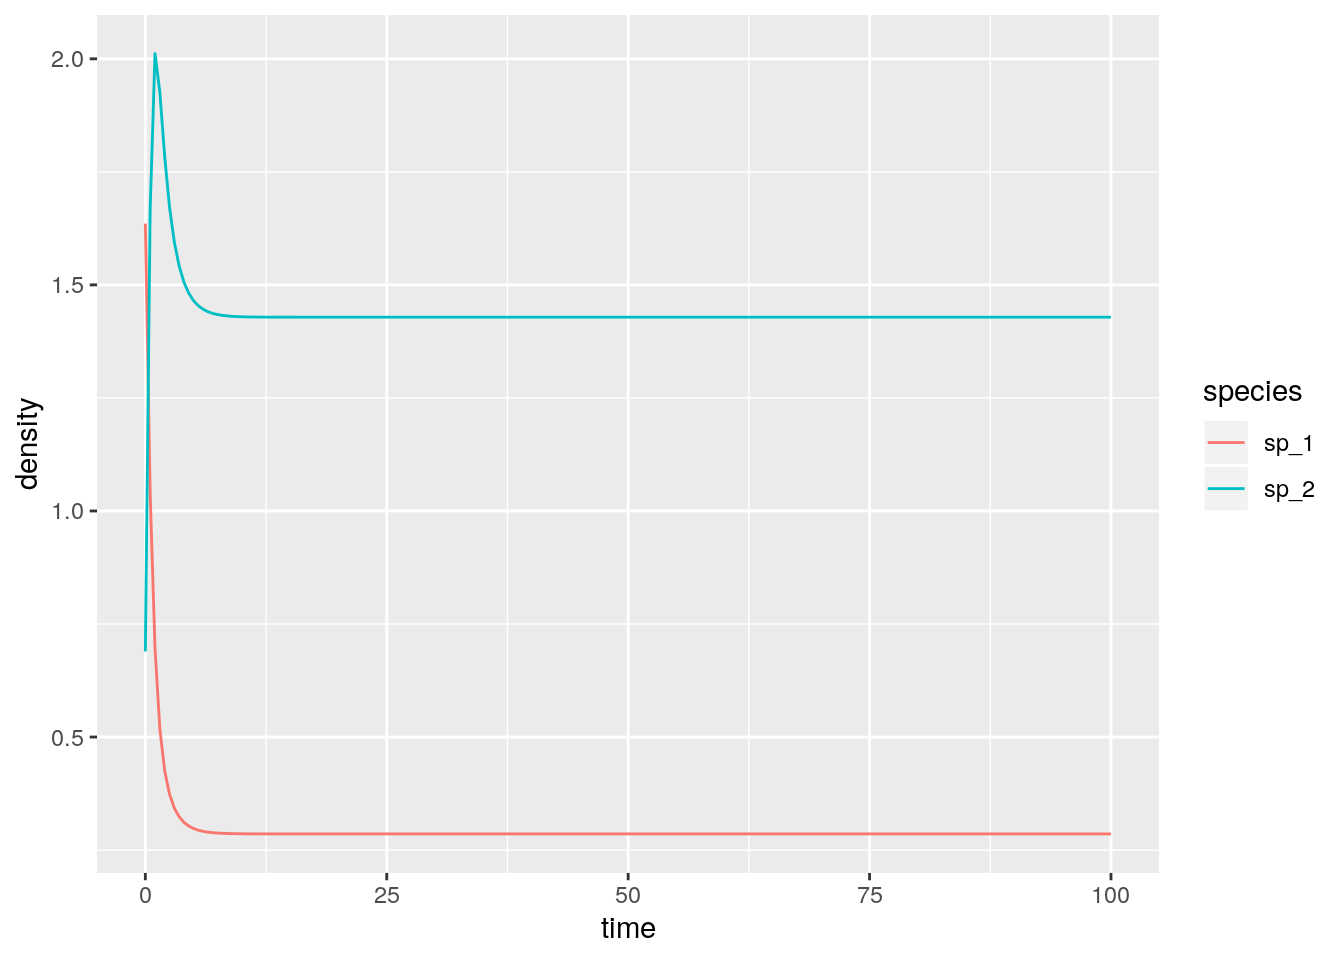
\includegraphics{A-Tour-of-the-Generalized-Lotka-Volterra-Model_files/figure-latex/globalst2-2} \end{center}

\begin{verbatim}
# [1] -1 -3
# [1] 0.2857143 1.4285714
\end{verbatim}

\hypertarget{stability-of-large-random-communities}{%
\section{Stability of large random communities}\label{stability-of-large-random-communities}}

As we have seen above, an equilibrium \(x^\star\) is stable if the community matrix for the equilibrium has all eigenvalues with negative real part. In general, to determine the equilibrium and its stability, we would need to specify all the growth rates (\(r\), \(n\) values), as well as the matrix of interactions (\(A\), \(n^2\) values). This is impractical to do for large systems (though we will try this out later). But can something quite general be said about the limit in which many species are in the community?

\citet{may1972will} attempted to answer this question by considering a \textbf{random community matrix}. In a GLV system, the diagonal elements \(m_{ii} = a_{ii} x_i^\star\) are influenced by self-regulation (i.e., as in a carrying capacity), while the off-diagonal elements \(m_{ij} = a_{ij} x_i^\star\) model the effect of species \(j\) on the equilibrium of species \(i\). May considered the following algorithm to build a random community matrix. Take a large community, resting at an unspecified equilibrium; we build the community matrix by setting

\begin{itemize}
\tightlist
\item
  \(m_{ij} = 0\) with probability \((1-C)\); with probability \(C\) we draw \(m_{ij}\) from a distribution with mean zero and variance \(\sigma^2\). \(C\) is the proportion of realized connections, termed the ``connectance'' of the system.
\item
  the diagonal elements are set to \(-d\), modeling self-regulation.
\end{itemize}

For example, the code uses a normal distribution:

\begin{Shaded}
\begin{Highlighting}[]
\NormalTok{build_May_normal <-}\StringTok{ }\ControlFlowTok{function}\NormalTok{(n, C, d, sigma)\{}
  \CommentTok{# fill the whole matrix}
\NormalTok{  M <-}\StringTok{ }\KeywordTok{matrix}\NormalTok{(}\KeywordTok{rnorm}\NormalTok{(n }\OperatorTok{*}\StringTok{ }\NormalTok{n, }\DataTypeTok{mean =} \DecValTok{0}\NormalTok{, }\DataTypeTok{sd =}\NormalTok{ sigma), n, n)}
  \CommentTok{# remove connections }
\NormalTok{  M <-}\StringTok{ }\NormalTok{M }\OperatorTok{*}\StringTok{ }\KeywordTok{matrix}\NormalTok{(}\KeywordTok{runif}\NormalTok{(n }\OperatorTok{*}\StringTok{ }\NormalTok{n) }\OperatorTok{<=}\StringTok{ }\NormalTok{C, n, n)}
  \CommentTok{# set diagonals}
  \KeywordTok{diag}\NormalTok{(M) <-}\StringTok{ }\OperatorTok{-}\NormalTok{d}
  \KeywordTok{return}\NormalTok{(M)}
\NormalTok{\}}
\end{Highlighting}
\end{Shaded}

We want to determine whether the equilibrium will be stable, given \(n\), \(C\), \(d\) and \(\sigma^2\). To do so, we need to find the location of the ``rightmost'' eigenvalue of \(M\). For example, let's plot the eigenvalues of a large matrix:

\begin{Shaded}
\begin{Highlighting}[]
\NormalTok{plot_eigenvalues <-}\StringTok{ }\ControlFlowTok{function}\NormalTok{(M, }\DataTypeTok{prediction =} \OtherTok{NULL}\NormalTok{)\{}
\NormalTok{  eig <-}\StringTok{ }\KeywordTok{eigen}\NormalTok{(M, }\DataTypeTok{only.values =} \OtherTok{TRUE}\NormalTok{)}\OperatorTok{$}\NormalTok{values}
\NormalTok{  dt <-}\StringTok{ }\KeywordTok{tibble}\NormalTok{(}\DataTypeTok{Real =} \KeywordTok{Re}\NormalTok{(eig), }\DataTypeTok{Imaginary =} \KeywordTok{Im}\NormalTok{(eig))}
\NormalTok{  pl <-}\StringTok{ }\KeywordTok{ggplot}\NormalTok{(dt) }\OperatorTok{+}\StringTok{ }\KeywordTok{aes}\NormalTok{(}\DataTypeTok{x =}\NormalTok{ Real, }\DataTypeTok{y =}\NormalTok{ Imaginary) }\OperatorTok{+}\StringTok{ }
\StringTok{    }\KeywordTok{geom_point}\NormalTok{() }\OperatorTok{+}\StringTok{ }
\StringTok{    }\KeywordTok{coord_equal}\NormalTok{() }\OperatorTok{+}\StringTok{ }
\StringTok{    }\KeywordTok{geom_vline}\NormalTok{(}\DataTypeTok{xintercept =} \DecValTok{0}\NormalTok{, }\DataTypeTok{colour =} \StringTok{"red"}\NormalTok{, }\DataTypeTok{linetype =} \DecValTok{2}\NormalTok{)}
  \ControlFlowTok{if}\NormalTok{ (}\KeywordTok{is.null}\NormalTok{(prediction) }\OperatorTok{==}\StringTok{ }\OtherTok{FALSE}\NormalTok{) \{}
\NormalTok{    pl <-}\StringTok{ }\NormalTok{pl }\OperatorTok{+}\StringTok{ }\KeywordTok{geom_vline}\NormalTok{(}\DataTypeTok{xintercept =}\NormalTok{ prediction, }\DataTypeTok{colour =} \StringTok{"black"}\NormalTok{, }\DataTypeTok{linetype =} \DecValTok{2}\NormalTok{)}
\NormalTok{  \}}
  \KeywordTok{show}\NormalTok{(pl)}
\NormalTok{\}}
\KeywordTok{set.seed}\NormalTok{(}\DecValTok{100}\NormalTok{) }\CommentTok{# for reproducibility}
\CommentTok{# parameters}
\NormalTok{n <-}\StringTok{ }\DecValTok{500}
\NormalTok{C <-}\StringTok{ }\FloatTok{0.5}
\NormalTok{d <-}\StringTok{ }\DecValTok{10}
\NormalTok{sigma <-}\StringTok{ }\DecValTok{1}
\NormalTok{M <-}\StringTok{ }\KeywordTok{build_May_normal}\NormalTok{(n, C, d, sigma)}
\KeywordTok{plot_eigenvalues}\NormalTok{(M)}
\end{Highlighting}
\end{Shaded}

\begin{center}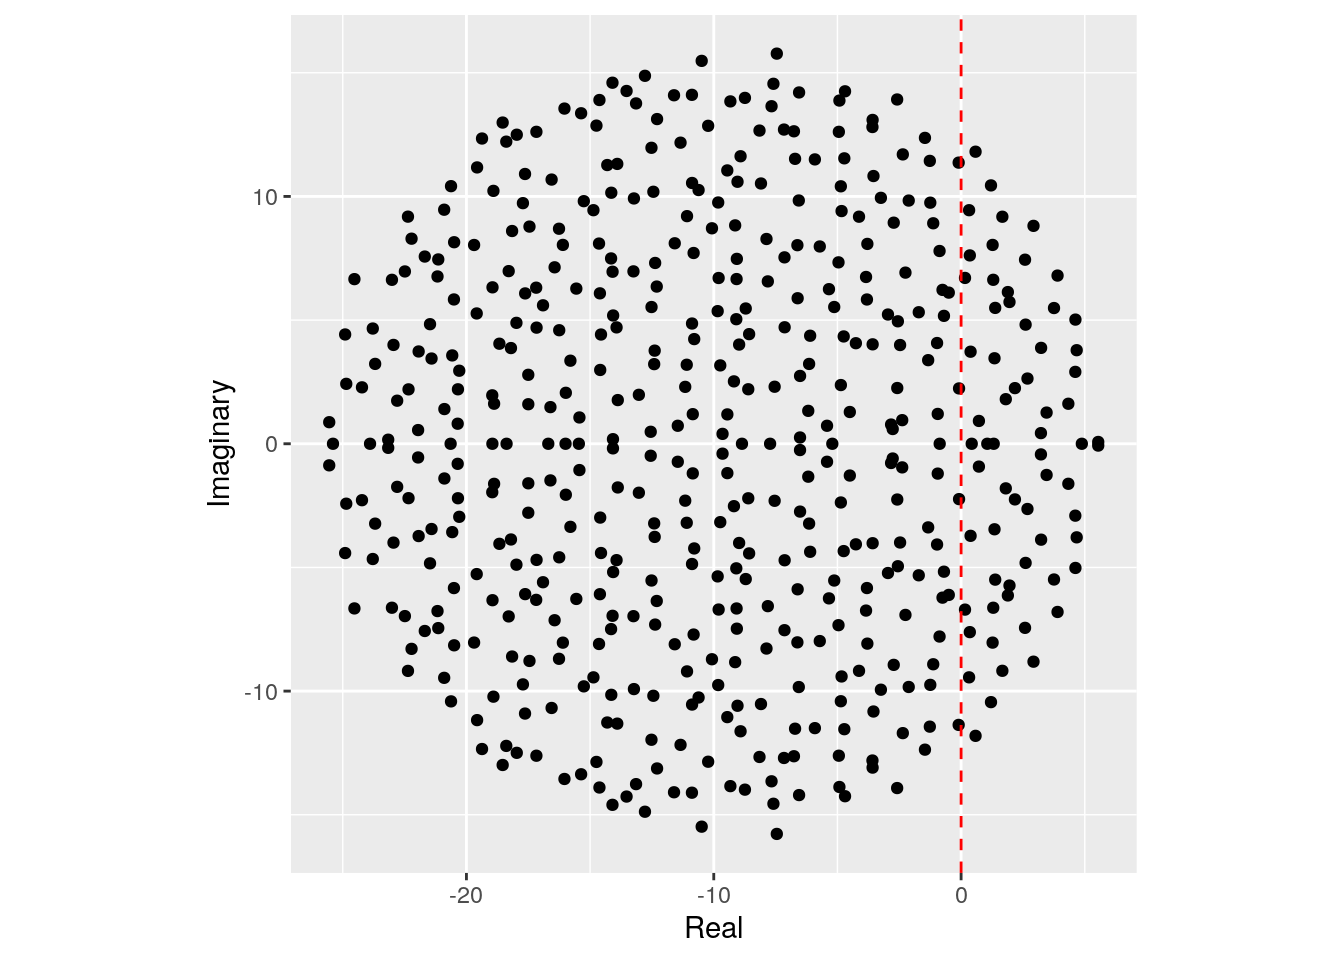
\includegraphics{A-Tour-of-the-Generalized-Lotka-Volterra-Model_files/figure-latex/exmay-1} \end{center}

The eigenvalues fall into an almost perfect circle! Turns out, that this is the behavior we should expect, as stated by the so-called ``Circular Law'', one of the most beautiful results in random matrix theory.

\textbf{Circular law:} Take a non-symmetric, \(S \times S\) random matrix in which all coefficients \(X_{ij}\) are i.i.d. random variables with \(\mathbb E[X_{ij}] = 0\) and \(\mathbb E[X_{ij}] = 1\). Then, as \(S \to \infty\), the e.s.d. of \({X} / \sqrt{S}\) converges to the circular law:

\[
  \mu(\lambda) = \begin{cases}
    \frac{1}{\pi} \; \; \; \text{if} \; (\text{Re}(\lambda))^2 +
    (\text{Im}(\lambda))^2 \leq 1\\
    0 \; \; \;\text{ otherwise}.
  \end{cases}
\]

This result can be used to calculate the radius of the eigenvalue distribution of the matrices studied by May: when the off-diagonal coefficients \(M_{ij}\) are 0 with probability \(1-C\) and are sampled independently from a distribution with mean \(0\) and variance \(\sigma^2\) with probability \(C\), we have that \(\mathbb E[M_{ij}] = 0\) and \(\mathbb E[M_{ij}^2] = C \sigma^2\). This means that if we were to divide the coefficients of \({M}\) by \(\sqrt{C \sigma^2}\) we would recover the unit variance, and the matrix would follow the circular law when \(S\) is large. Armed with this, we can calculate the radius: if the radius of \({M} / \sqrt{S C \sigma^2}\) converges to 1 when the matrix is large, then the radius of \({M}\) is approximately \(\sqrt{S C \sigma^2}\). For stability, we need a sufficiently negative diagonal, yielding May's stability criterion:

\[
\sqrt{S C \sigma^2} < d
\]

We can try this on our matrix:

\begin{Shaded}
\begin{Highlighting}[]
\NormalTok{prediction <-}\StringTok{ }\KeywordTok{sqrt}\NormalTok{(n }\OperatorTok{*}\StringTok{ }\NormalTok{C }\OperatorTok{*}\StringTok{ }\NormalTok{sigma}\OperatorTok{^}\DecValTok{2}\NormalTok{) }\OperatorTok{-}\StringTok{ }\NormalTok{d}
\KeywordTok{plot_eigenvalues}\NormalTok{(M, prediction)}
\end{Highlighting}
\end{Shaded}

\begin{center}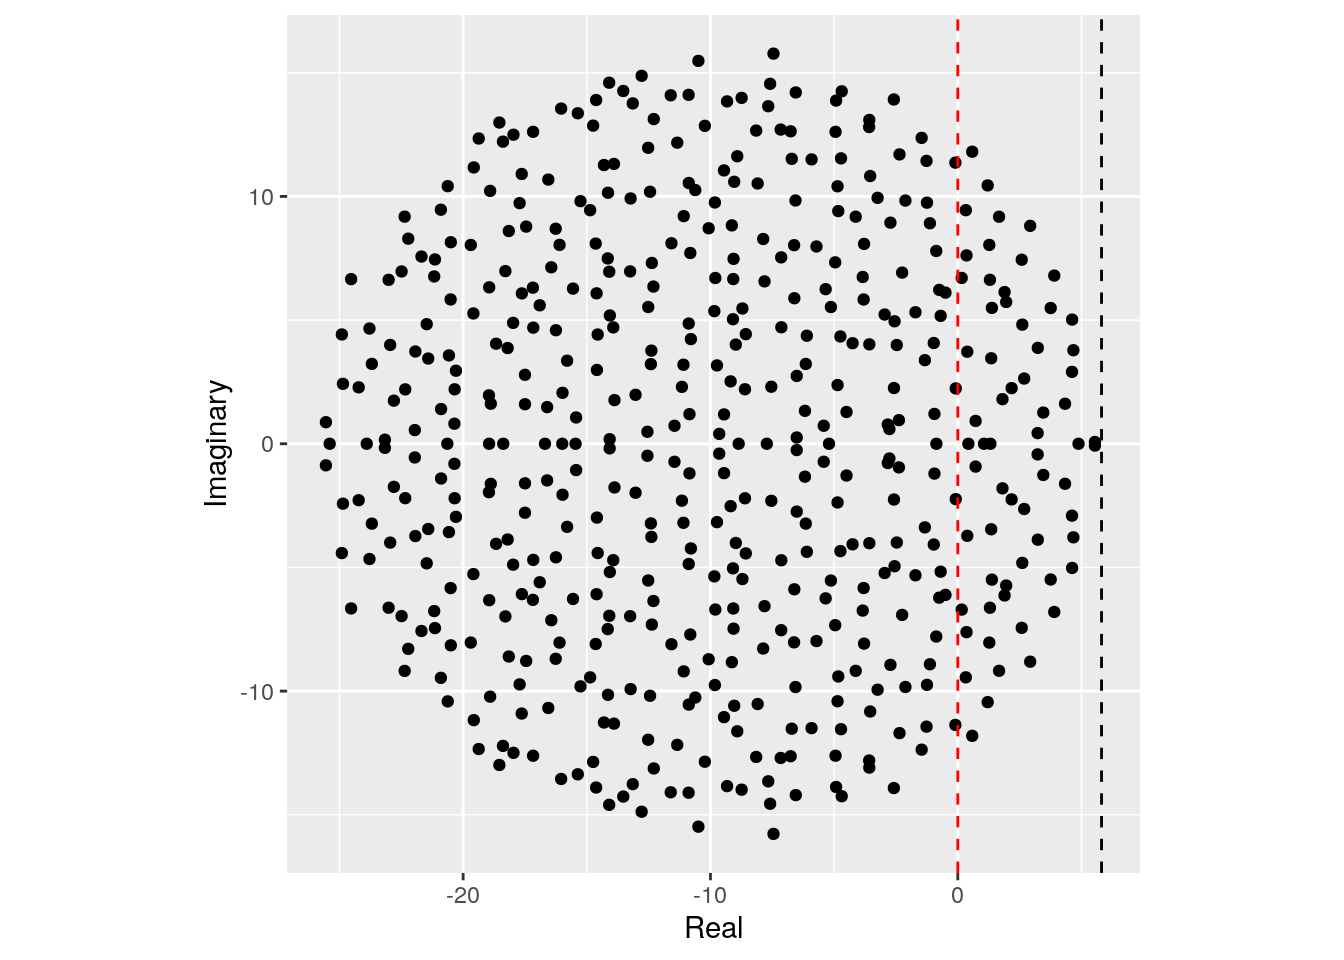
\includegraphics{A-Tour-of-the-Generalized-Lotka-Volterra-Model_files/figure-latex/maycrit-1} \end{center}

Showing that we accurately approximate the location of the rightmost eigenvalue. Note that, in the case of large \(n\), whenever the circle crosses zero, some eigenvalues will be positive, determining the instability of the equilibrium.

Importantly, the distribution from which the coefficients are sampled does not matter---only that the mean is zero and that the variance is \(\sigma^2\). For example, build the matrix using coefficients from a uniform distribution:

\begin{Shaded}
\begin{Highlighting}[]
\NormalTok{build_May_uniform <-}\StringTok{ }\ControlFlowTok{function}\NormalTok{(n, C, d, sigma)\{}
  \CommentTok{# fill the whole matrix (sqrt(3) to ensure var = sigma^2)}
\NormalTok{  M <-}\StringTok{ }\KeywordTok{matrix}\NormalTok{(}\KeywordTok{runif}\NormalTok{(n }\OperatorTok{*}\StringTok{ }\NormalTok{n, }\DataTypeTok{min =} \OperatorTok{-}\KeywordTok{sqrt}\NormalTok{(}\DecValTok{3}\NormalTok{) }\OperatorTok{*}\StringTok{ }\NormalTok{sigma, }\DataTypeTok{max =} \KeywordTok{sqrt}\NormalTok{(}\DecValTok{3}\NormalTok{) }\OperatorTok{*}\StringTok{ }\NormalTok{sigma), n, n)}
  \CommentTok{# remove connections }
\NormalTok{  M <-}\StringTok{ }\NormalTok{M }\OperatorTok{*}\StringTok{ }\KeywordTok{matrix}\NormalTok{(}\KeywordTok{runif}\NormalTok{(n }\OperatorTok{*}\StringTok{ }\NormalTok{n) }\OperatorTok{<=}\StringTok{ }\NormalTok{C, n, n)}
  \CommentTok{# set diagonals}
  \KeywordTok{diag}\NormalTok{(M) <-}\StringTok{ }\OperatorTok{-}\NormalTok{d}
  \KeywordTok{return}\NormalTok{(M)}
\NormalTok{\}}
\CommentTok{# parameters}
\NormalTok{n <-}\StringTok{ }\DecValTok{500}
\NormalTok{C <-}\StringTok{ }\FloatTok{0.5}
\NormalTok{d <-}\StringTok{ }\DecValTok{10}
\NormalTok{sigma <-}\StringTok{ }\DecValTok{1}
\NormalTok{M <-}\StringTok{ }\KeywordTok{build_May_uniform}\NormalTok{(n, C, d, sigma)}
\NormalTok{prediction <-}\StringTok{ }\KeywordTok{sqrt}\NormalTok{(n }\OperatorTok{*}\StringTok{ }\NormalTok{C }\OperatorTok{*}\StringTok{ }\NormalTok{sigma}\OperatorTok{^}\DecValTok{2}\NormalTok{) }\OperatorTok{-}\StringTok{ }\NormalTok{d}
\KeywordTok{plot_eigenvalues}\NormalTok{(M, prediction)}
\end{Highlighting}
\end{Shaded}

\begin{center}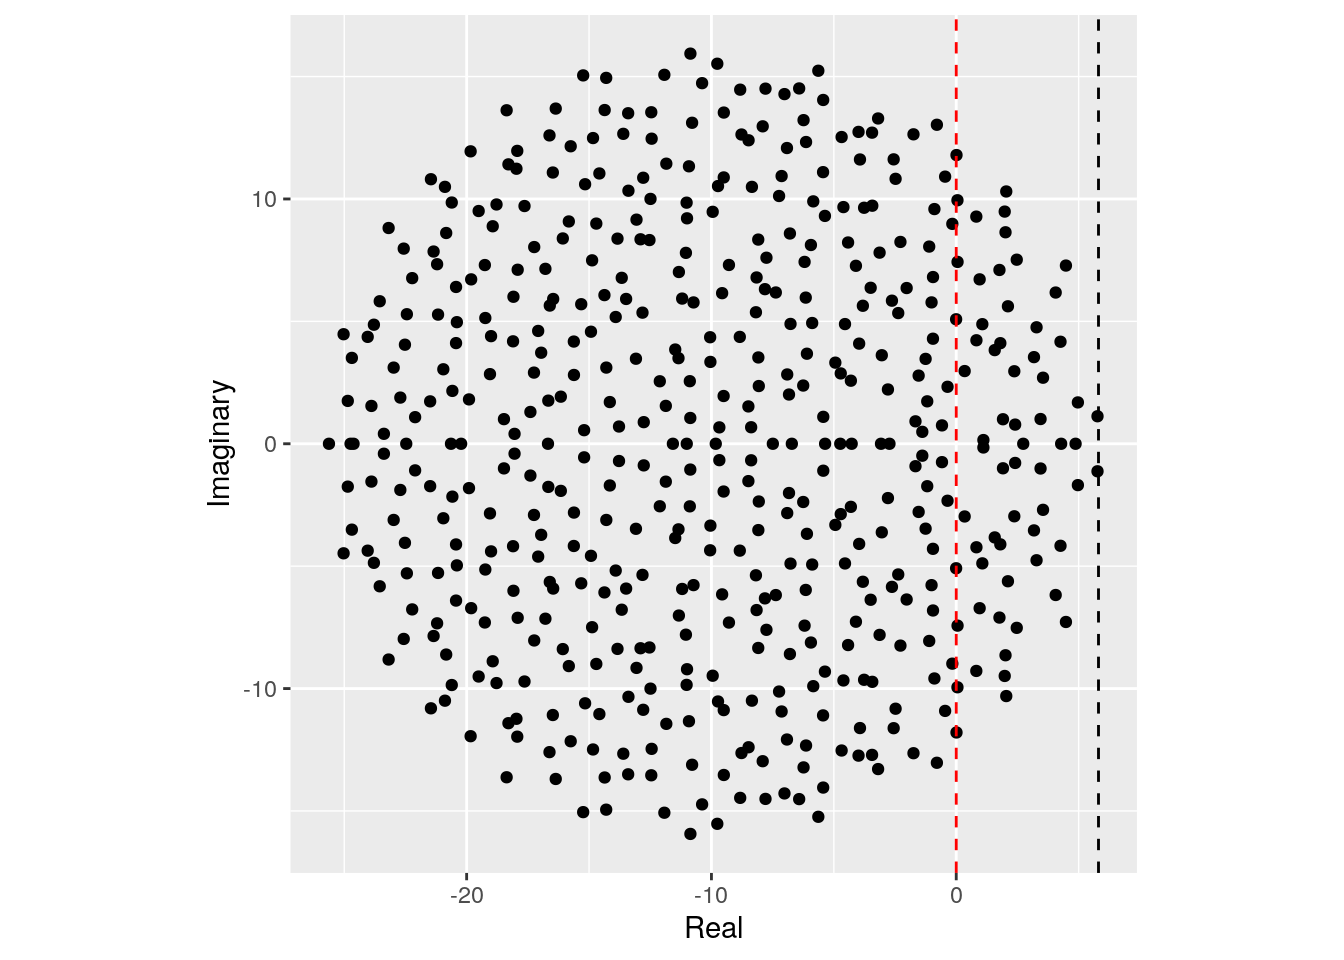
\includegraphics{A-Tour-of-the-Generalized-Lotka-Volterra-Model_files/figure-latex/exmay2-1} \end{center}

This property is called \textbf{universality} in random matrix theory.

In ecological communities, the effect of species \(i\) on \(j\) and that of \(j\) on \(i\) are typically not independent (as assumed above): in the case of competition between species, we expect them both to be negative; for consumption, if one is positive, the other is negative, and so forth. A more refined model of a random matrix would therefore sample interactions in pairs from a bivariate distribution. The elliptic law can deal with this case:

\textbf{Elliptic law:} Take a non-symmetric, \(S \times S\) random matrix in which the pairs of coefficients \((X_{ij}, X_{ji})\) are sampled independently from a bivariate distribution defined by a vector of means \(m = (0,0)^t\) and a covariance matrix \(\Sigma = \begin{pmatrix} 1 & \rho\\ \rho & 1 \end{pmatrix}\). Then, as \(S \to \infty\), the e.s.d. of \({X} / \sqrt{S}\) converges to the elliptic law:

\[
  \mu(\lambda) = \begin{cases} \frac{1}{\pi (1 - \rho^2) } \quad
    \text{if} \; \frac{(\text{Re}(\lambda))^2}{(1 + \rho)^2} +
    \frac{(\text{Im}(\lambda))^2}{(1 -\rho)^2} \leq
    1\\ 0 \quad \quad \quad \text{ otherwise}
  \end{cases}
\]

Note that when \(\rho = 0\), the elliptic law reduces to the circular law. Using the elliptic law, \citet{allesina2012stability} were able to extend May's criterion to ecological networks with different mixtures of interaction types. In particular, the stability criterion becomes:

\[
\sqrt{S C \sigma^2}(1 + \rho) < d
\]

To see the elliptic law in action, we can build matrices in which we sample the coefficients in pairs from a bivariate normal distribution:

\begin{Shaded}
\begin{Highlighting}[]
\NormalTok{build_Allesina_Tang_normal <-}\StringTok{ }\ControlFlowTok{function}\NormalTok{(n, C, d, sigma, rho)\{}
  \CommentTok{# sample coefficients in pairs}
\NormalTok{  pairs <-}\StringTok{ }\NormalTok{MASS}\OperatorTok{::}\KeywordTok{mvrnorm}\NormalTok{(}\DataTypeTok{n =}\NormalTok{ n }\OperatorTok{*}\StringTok{ }\NormalTok{(n}\DecValTok{-1}\NormalTok{) }\OperatorTok{/}\StringTok{ }\DecValTok{2}\NormalTok{,}
                         \DataTypeTok{mu =} \KeywordTok{c}\NormalTok{(}\DecValTok{0}\NormalTok{, }\DecValTok{0}\NormalTok{),}
                         \DataTypeTok{Sigma =}\NormalTok{ sigma}\OperatorTok{^}\DecValTok{2} \OperatorTok{*}\StringTok{ }\KeywordTok{matrix}\NormalTok{(}\KeywordTok{c}\NormalTok{(}\DecValTok{1}\NormalTok{, rho, rho, }\DecValTok{1}\NormalTok{), }\DecValTok{2}\NormalTok{, }\DecValTok{2}\NormalTok{))}
  \CommentTok{# build a completely filled matrix}
\NormalTok{  M <-}\StringTok{ }\KeywordTok{matrix}\NormalTok{(}\DecValTok{0}\NormalTok{, n, n)}
\NormalTok{  M[}\KeywordTok{upper.tri}\NormalTok{(M)] <-}\StringTok{ }\NormalTok{pairs[,}\DecValTok{1}\NormalTok{]}
\NormalTok{  M <-}\StringTok{ }\KeywordTok{t}\NormalTok{(M)}
\NormalTok{  M[}\KeywordTok{upper.tri}\NormalTok{(M)] <-}\StringTok{ }\NormalTok{pairs[,}\DecValTok{2}\NormalTok{]}
  \CommentTok{# determine which connections to retain}
\NormalTok{  Connections <-}\StringTok{ }\NormalTok{(}\KeywordTok{matrix}\NormalTok{(}\KeywordTok{runif}\NormalTok{(n }\OperatorTok{*}\StringTok{ }\NormalTok{n), n, n) }\OperatorTok{<=}\StringTok{ }\NormalTok{C) }\OperatorTok{*}\StringTok{ }\DecValTok{1} 
\NormalTok{  Connections[}\KeywordTok{lower.tri}\NormalTok{(Connections)] <-}\StringTok{ }\DecValTok{0}
  \KeywordTok{diag}\NormalTok{(Connections) <-}\StringTok{ }\DecValTok{0}
\NormalTok{  Connections <-}\StringTok{ }\NormalTok{Connections }\OperatorTok{+}\StringTok{ }\KeywordTok{t}\NormalTok{(Connections)}
\NormalTok{  M <-}\StringTok{ }\NormalTok{M }\OperatorTok{*}\StringTok{ }\NormalTok{Connections}
  \KeywordTok{diag}\NormalTok{(M) <-}\StringTok{ }\OperatorTok{-}\NormalTok{d}
  \KeywordTok{return}\NormalTok{(M)}
\NormalTok{\}}
\end{Highlighting}
\end{Shaded}

We can see that a positive connectance leads to an eigenvalue distribution that describes an horizontally-stretched ellipse (and hence, more difficult to stabilize than the circle):

\begin{Shaded}
\begin{Highlighting}[]
\CommentTok{# parameters}
\NormalTok{n <-}\StringTok{ }\DecValTok{500}
\NormalTok{C <-}\StringTok{ }\FloatTok{0.5}
\NormalTok{d <-}\StringTok{ }\DecValTok{10}
\NormalTok{sigma <-}\StringTok{ }\DecValTok{1}
\NormalTok{rho <-}\StringTok{ }\FloatTok{0.4}
\NormalTok{M <-}\StringTok{ }\KeywordTok{build_Allesina_Tang_normal}\NormalTok{(n, C, d, sigma, rho)}
\NormalTok{prediction <-}\StringTok{ }\KeywordTok{sqrt}\NormalTok{(n }\OperatorTok{*}\StringTok{ }\NormalTok{C }\OperatorTok{*}\StringTok{ }\NormalTok{sigma}\OperatorTok{^}\DecValTok{2}\NormalTok{) }\OperatorTok{*}\StringTok{ }\NormalTok{(}\DecValTok{1} \OperatorTok{+}\StringTok{ }\NormalTok{rho) }\OperatorTok{-}\StringTok{ }\NormalTok{d}
\KeywordTok{plot_eigenvalues}\NormalTok{(M, prediction)}
\end{Highlighting}
\end{Shaded}

\begin{center}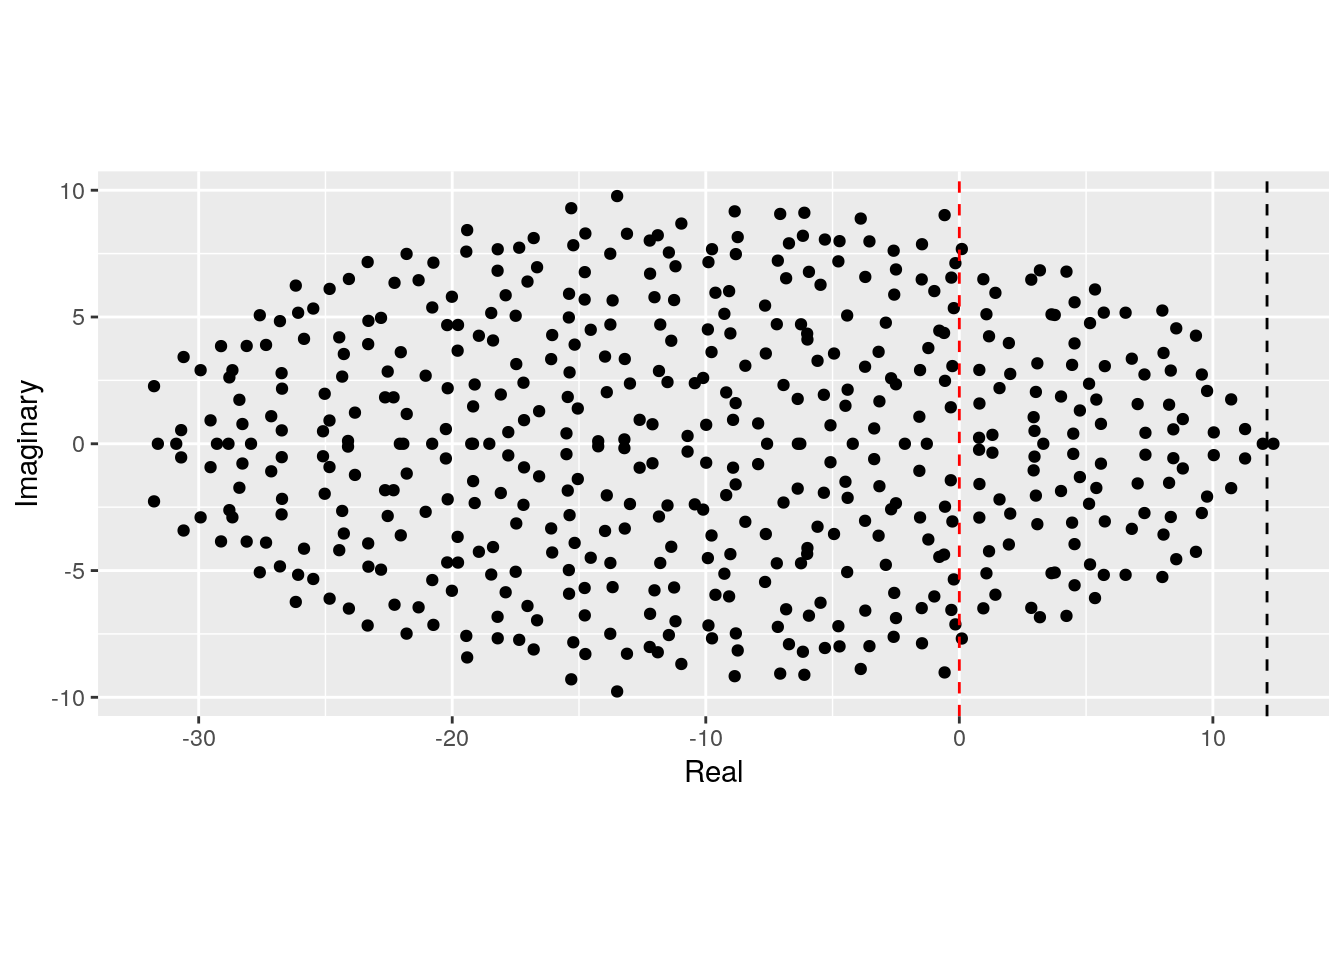
\includegraphics{A-Tour-of-the-Generalized-Lotka-Volterra-Model_files/figure-latex/allesinatangex1-1} \end{center}

Similarly, a negative correlation (e.g., as in predator-prey) would make the system easier to stabilize:

\begin{Shaded}
\begin{Highlighting}[]
\CommentTok{# parameters}
\NormalTok{n <-}\StringTok{ }\DecValTok{500}
\NormalTok{C <-}\StringTok{ }\FloatTok{0.5}
\NormalTok{d <-}\StringTok{ }\DecValTok{10}
\NormalTok{sigma <-}\StringTok{ }\DecValTok{1}
\NormalTok{rho <-}\StringTok{ }\FloatTok{-0.4}
\NormalTok{M <-}\StringTok{ }\KeywordTok{build_Allesina_Tang_normal}\NormalTok{(n, C, d, sigma, rho)}
\NormalTok{prediction <-}\StringTok{ }\KeywordTok{sqrt}\NormalTok{(n }\OperatorTok{*}\StringTok{ }\NormalTok{C }\OperatorTok{*}\StringTok{ }\NormalTok{sigma}\OperatorTok{^}\DecValTok{2}\NormalTok{) }\OperatorTok{*}\StringTok{ }\NormalTok{(}\DecValTok{1} \OperatorTok{+}\StringTok{ }\NormalTok{rho) }\OperatorTok{-}\StringTok{ }\NormalTok{d}
\KeywordTok{plot_eigenvalues}\NormalTok{(M, prediction)}
\end{Highlighting}
\end{Shaded}

\begin{center}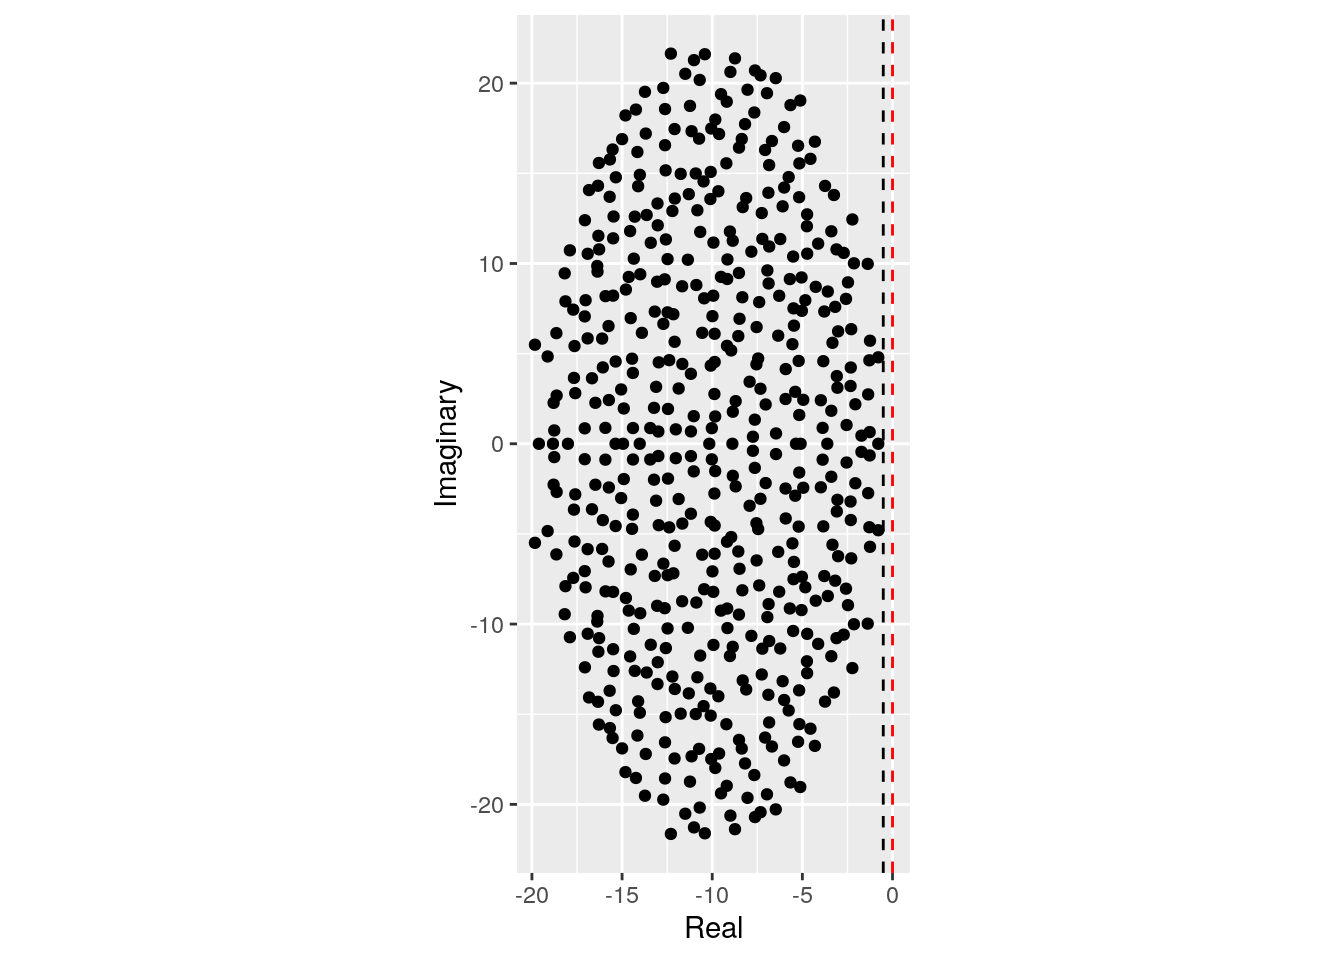
\includegraphics{A-Tour-of-the-Generalized-Lotka-Volterra-Model_files/figure-latex/allesinatangex2-1} \end{center}

\hypertarget{further-readings}{%
\section{Further readings}\label{further-readings}}

On the theory of GLV:

\begin{itemize}
\item
  \citet{strogatz2018nonlinear} is a simple introduction to dynamical systems and bifurcation theory.
\item
  \citet{hofbauer1998evolutionary} is a wonderful introduction to dynamical systems in ecology and population genetics, with a nice introduction to evolutionary game theory.
\item
  \citet{hadeler2017topics} contains a more mathematically-oriented treatment of the material covered in the first part of this lecture.
\item
  \citet{baigent2016lotka} is a mathematical introduction to Lotka-Volterra dynamics.
\end{itemize}

On random matrices and stability:

\begin{itemize}
\tightlist
\item
  \citet{allesina2015stability} is an opinionated review on applications of random matrices in ecology.
\end{itemize}

\hypertarget{multi}{%
\chapter{Multispecies GLV}\label{multi}}

\hypertarget{feasibility}{%
\section{Feasibility}\label{feasibility}}

\hypertarget{stability}{%
\section{Stability}\label{stability}}

\hypertarget{non-invasibility}{%
\section{Non-invasibility}\label{non-invasibility}}

\hypertarget{assembly}{%
\section{Assembly}\label{assembly}}

\hypertarget{a-random-zoo}{%
\section{A random zoo}\label{a-random-zoo}}

\hypertarget{games}{%
\chapter{Evolutionary Game Theory}\label{games}}

\hypertarget{game-theory}{%
\section{Game theory}\label{game-theory}}

We briefly introduce the study of mathematical models of games, and their relations to the GLV model. While the origin of game theory can be traced back to the 1700s, modern game theory started with von Neumann's paper \emph{On the Theory of Games of Strategy}, published in 1928, and with the subsequent 1944 book with Morgensten \emph{Theory of Games and Economic Behavior}. John Nash's paper \citep{nash1950equilibrium} introduced the notion of a \textbf{Nash Equilibrium} (NE). Originally, game theory was studied by economists and mathematicians, but with the 1973 book \emph{Evolution and the Theory of Games} \citep{smith1982evolution}, John Maynard Smith showed how the same tools could be used to study evolutionary dynamics, introducing the influential concept of an \textbf{Evolutionary Stable Strategy} (ESS). Evolutionary game theory was greatly advanced through the introduction of the \textbf{Replicator Equation} (RE), which, as we will see later, has strong connection with the GLV model. For a detailaed introduction to evolutionary game theory see \citet{hofbauer1998evolutionary}.

\hypertarget{two-player-matrix-games}{%
\section{Two-player matrix games}\label{two-player-matrix-games}}

We start by anayzing games in which two players face each other, each choosing one strategy out of a set. Importantly, we consider static games in which each player makes their decision without having knowledge of the decision of the other player. Player 1 chooses a ``pure'' strategy \(s_1\) from the set of pure strategies \(S_1\), while player 2 chooses \(s_2 \in S_2\). We call \(\pi_k (s_1, s_2)\) the \textbf{payoff} for player \(k\) when player 1 chooses \(s_1\) and player 2 \(s_2\). In a matrix game, we can arrange the payoffs for each player in a matrix. We call \(A\) the matrix of payoffs for player one and \(B\) that for player two.

\hypertarget{example-the-prisoners-dilemma}{%
\subsection{Example: the prisoner's dilemma}\label{example-the-prisoners-dilemma}}

Two prisoners alleggedly committed a crime, but the police do not have enough evidence to convict them. They therefore approach each player separately, proposing a deal: if the prisoner confesses (``defect'' the other prisoner), then their sentence will be reduced. In particular: i) if both confess (both ``defect''), they are sentenced to 4 years in prison; ii) if one confesses (``defect'') and the other keeps quiet (``cooperate'' with the other prisoner), then the one who has confessed is let free, and the other sentenced to 5 years; iii) if both keep quiet (``cooperate''), then they are both sentenced to two years of detention for some accessory crime.

In matrix form, we have (rows for pl 1 strategy C/D; cols for pl 2 strategy):

\[
A = \begin{pmatrix}
-2 & -5\\
0 & -4
\end{pmatrix} \quad
B = \begin{pmatrix}
-2 & -5\\
0 & -4
\end{pmatrix}
\]

What is the best strategy player 1 can play---without knowing whether player 2 will confess or not? If player 2 were to keep quiet, player 1 should confess and be let free; if player 2 confesses, on the other hand, player 1 should also confess and get a reduced sentence. As such, each player would rationally choose to confess, thereby getting sentenced to four years in prison; note that if they could trust the other player, they could cooperate to get a much reduced sentence.

The defect/defect is called a \textbf{Nash Equilibrium}: no player can improve their payoff by changing only their own strategy.

\hypertarget{mixed-strategies}{%
\section{Mixed strategies}\label{mixed-strategies}}

Above, the player could choose one out of two strategies. A generalization of this situation is one in which players play \textbf{mixed} strategies, i.e., play a given strategy at random according to a set of probabilities. Call \(x_i\) the probability that player 1 plays strategy \(i\); then \(\sum_i x_i = 1\). Similarly, \(y_i\) is the probability that player 2 plays strategy \(i\). A natural choice for the payoff of player 1 is therefore:

\[
\sum_{i=1}^m \sum_{j = 1}^n x_i y_j \pi_1 (s_1, s_2) = x^t A y
\]
Similarly, we have \(y^t B x\) for player 2.

A mixed strategy \(x\) is dominated by mixed strategy \(\tilde{x}\) if \(\tilde{x}^t A y \geq x A y\) for every \(y\). The condition can be written as \((\tilde{x}^t - x) A y \geq 0\).

\hypertarget{nash-equilibria}{%
\section{Nash Equilibria}\label{nash-equilibria}}

A pair of mixed strategies \(\tilde{x}\) and \(\tilde{y}\) is called a Nash Equilibrium for a two person matrix game if:

\[
\begin{aligned}
\tilde{x}^t A \tilde{y} \geq x^t A \tilde{y} &\quad \text{for all } x\\
\tilde{y}^t B \tilde{x} \geq y^t B \tilde{x} &\quad \text{for all } y
\end{aligned}
\]

Nash proved that every two-person game has at least one Nash Equilibrium.

\hypertarget{evolutionary-stable-strategies}{%
\section{Evolutionary stable strategies}\label{evolutionary-stable-strategies}}

In the context of evolution, one can consider \(x\) to be the proportion of individuals (e.g., of different species, or phenotypes) displaying different characteristics. When playing against each other, they win or lose, and their payoffs are invested in reproduction. Because the different ``strategies'' (populations, phenotypes) play against each other, the payoff matrix is the same for all players, and encoded in matrix \(A\).

In this context, a strategy \(x\) is called an evolutionary stable strategy if two conditions are met:
\[
x^t A x \geq y^t A x \quad \text{for all } y
\]
meaning that \(x\) plays against itself not worse than any other strategy, and

\[
\text{If } y \neq x \text{ then } y^t A x = x^t A x \text{ implies } x^t A y > y^t A y
\]

meaning that if \(y\) plays as well as \(x\) against \(x\), then \(x\) plays against \(y\) better than \(y\) against itself.

We next connect NE and ESS with dynamical systems.

\hypertarget{replicator-dynamics}{%
\section{Replicator dynamics}\label{replicator-dynamics}}

The replicator equation can be written as:

\[
\dfrac{d x}{dt} = D(x)(A x - x^t A x)
\]

Where \(f = A x\) is a vector reporting the fitness of each population at time \(t\), and \(\bar{f} = x^t A t\) is the average fitness at time \(t\). As such, one can write the replicator equation more compactly as:

\[
\dfrac{d x_i}{dt} = x_i (f_i - \bar{f})
\]

The RE is essentially equivalent to a GLV model in which we track frequencies instead of abundances.

Importantly, we can see \(x\) as a ``mixed strategy'' for the symmetric game encoded in \(A\). In this context, \textbf{an equilibrium of the replicator equation is a Nash Equilibrium for the game}; similarly, \textbf{a stable equilibrium for the replicator equation is an Evolutionary Stable Strategy}.

\hypertarget{invariants}{%
\subsection{Invariants}\label{invariants}}

Adding a constant to each column of \(A\) does not alter the dynamics. We have \(B = A + e b^t\), where \(e\) is a vector of ones. Then:

\[
\begin{aligned}
D(x)(B x - x^t B x) &= D(x)(A + eb^t) x - x^t (A + eb^t) x\\
&= D(x)A x + D(x) eb^t x - x^t A x - x^t e b^t x\\
&= D(x)A x + x^t e b^t x - x^t A x - x^t e b^t  x\\
&= D(x)A - x^t A x\\
&= D(x)(A x - x^t A x)
\end{aligned}
\]

Similarly, multiplying each column of \(A\) by a (possibly different) positive constant does not alter dynamics (it just rescales time). As such, if \(A_2 = A_1 D + eb^t\) the replicator equations formed using \(A_1\) and \(A_2\) are equivalent.

\hypertarget{rock-paper-scissor}{%
\subsection{Rock-paper-scissor}\label{rock-paper-scissor}}

Let's try our hand with a simple zero-sum (i.e., \(A = -A^t\)) replicator equation. We have three populations (``rock'', ``paper'', and ``scissors'') with payoff matrix:

\[
A = \begin{pmatrix}
0 & -1 & 1\\
1 & 0 & -1\\
-1 & 1 & 0
\end{pmatrix}
\]

We start the population at a random initial condition, and track dynamics:

\begin{Shaded}
\begin{Highlighting}[]
\KeywordTok{library}\NormalTok{(deSolve) }\CommentTok{# integrate ODEs}
\KeywordTok{library}\NormalTok{(tidyverse) }\CommentTok{# plotting and wrangling}
\CommentTok{# define the differential equation}
\NormalTok{RE <-}\ControlFlowTok{function}\NormalTok{(t, x, parameters)\{}
  \KeywordTok{with}\NormalTok{(}\KeywordTok{as.list}\NormalTok{(}\KeywordTok{c}\NormalTok{(x, parameters)), \{}
\NormalTok{    x[x }\OperatorTok{<}\StringTok{ }\DecValTok{10}\OperatorTok{^-}\DecValTok{8}\NormalTok{] <-}\StringTok{ }\DecValTok{0} \CommentTok{# prevent numerical problems}
\NormalTok{    x <-}\StringTok{ }\NormalTok{x }\OperatorTok{/}\StringTok{ }\KeywordTok{sum}\NormalTok{(x) }\CommentTok{# keep on simplex}
\NormalTok{    dxdt <-}\StringTok{ }\NormalTok{x }\OperatorTok{*}\StringTok{ }\NormalTok{(A }\OperatorTok\StringTok{ }\NormalTok{x }\OperatorTok{-}\StringTok{ }\KeywordTok{sum}\NormalTok{(x }\OperatorTok{*}\StringTok{ }\NormalTok{A }\OperatorTok\StringTok{ }\NormalTok{x))}
    \KeywordTok{list}\NormalTok{(dxdt)}
\NormalTok{  \})}
\NormalTok{\}}
\CommentTok{# function to plot output}
\NormalTok{plot_ODE_output <-}\StringTok{ }\ControlFlowTok{function}\NormalTok{(out)\{}
\NormalTok{  out <-}\StringTok{ }\KeywordTok{as.data.frame}\NormalTok{(out)}
  \KeywordTok{colnames}\NormalTok{(out) <-}\StringTok{ }\KeywordTok{c}\NormalTok{(}\StringTok{"time"}\NormalTok{, }\KeywordTok{paste}\NormalTok{(}\StringTok{"sp"}\NormalTok{, }\DecValTok{1}\OperatorTok{:}\NormalTok{(}\KeywordTok{ncol}\NormalTok{(out) }\DecValTok{-1}\NormalTok{), }\DataTypeTok{sep =} \StringTok{"_"}\NormalTok{))}
\NormalTok{  out <-}\StringTok{ }\KeywordTok{as_tibble}\NormalTok{(out) }\OperatorTok\StringTok{ }\KeywordTok{gather}\NormalTok{(species, density, }\OperatorTok{-}\NormalTok{time)}
\NormalTok{  pl <-}\StringTok{ }\KeywordTok{ggplot}\NormalTok{(}\DataTypeTok{data =}\NormalTok{ out) }\OperatorTok{+}\StringTok{ }
\StringTok{    }\KeywordTok{aes}\NormalTok{(}\DataTypeTok{x =}\NormalTok{ time, }\DataTypeTok{y =}\NormalTok{ density, }\DataTypeTok{colour =}\NormalTok{ species) }\OperatorTok{+}\StringTok{ }
\StringTok{    }\KeywordTok{geom_line}\NormalTok{()}
  \KeywordTok{show}\NormalTok{(pl)}
  \KeywordTok{return}\NormalTok{(out)}
\NormalTok{\}}
\CommentTok{# general function to integrate RE}
\NormalTok{integrate_RE <-}\StringTok{ }\ControlFlowTok{function}\NormalTok{(A, x0, }\DataTypeTok{maxtime =} \DecValTok{40}\NormalTok{, }\DataTypeTok{steptime =} \FloatTok{0.05}\NormalTok{)\{}
\NormalTok{  times <-}\StringTok{ }\KeywordTok{seq}\NormalTok{(}\DecValTok{0}\NormalTok{, maxtime, }\DataTypeTok{by =}\NormalTok{ steptime)}
\NormalTok{  parameters <-}\StringTok{ }\KeywordTok{list}\NormalTok{(}\DataTypeTok{A =}\NormalTok{ A)}
  \CommentTok{# solve numerically}
\NormalTok{  out <-}\StringTok{ }\KeywordTok{ode}\NormalTok{(}\DataTypeTok{y =}\NormalTok{ x0, }\DataTypeTok{times =}\NormalTok{ times, }
           \DataTypeTok{func =}\NormalTok{ RE, }\DataTypeTok{parms =}\NormalTok{ parameters, }
           \DataTypeTok{method =} \StringTok{"ode45"}\NormalTok{)}
  \CommentTok{# plot and make into tidy form}
\NormalTok{  out <-}\StringTok{ }\KeywordTok{plot_ODE_output}\NormalTok{(out)}
  \KeywordTok{return}\NormalTok{(out)}
\NormalTok{\}}
\CommentTok{# payoff matrix}
\NormalTok{A <-}\StringTok{ }\KeywordTok{matrix}\NormalTok{(}\KeywordTok{c}\NormalTok{(}\DecValTok{0}\NormalTok{, }\DecValTok{-1}\NormalTok{, }\DecValTok{1}\NormalTok{,}
              \DecValTok{1}\NormalTok{, }\DecValTok{0}\NormalTok{, }\DecValTok{-1}\NormalTok{,}
              \DecValTok{-1}\NormalTok{, }\DecValTok{1}\NormalTok{, }\DecValTok{0}\NormalTok{), }\DecValTok{3}\NormalTok{, }\DecValTok{3}\NormalTok{, }\DataTypeTok{byrow =} \OtherTok{TRUE}\NormalTok{)}
\CommentTok{# initial conditions}
\NormalTok{x0 <-}\StringTok{ }\KeywordTok{runif}\NormalTok{(}\DecValTok{3}\NormalTok{)}
\NormalTok{x0 <-}\StringTok{ }\NormalTok{x0 }\OperatorTok{/}\StringTok{ }\KeywordTok{sum}\NormalTok{(x0)}
\NormalTok{rps <-}\StringTok{ }\KeywordTok{integrate_RE}\NormalTok{(A, x0)}
\end{Highlighting}
\end{Shaded}

\begin{center}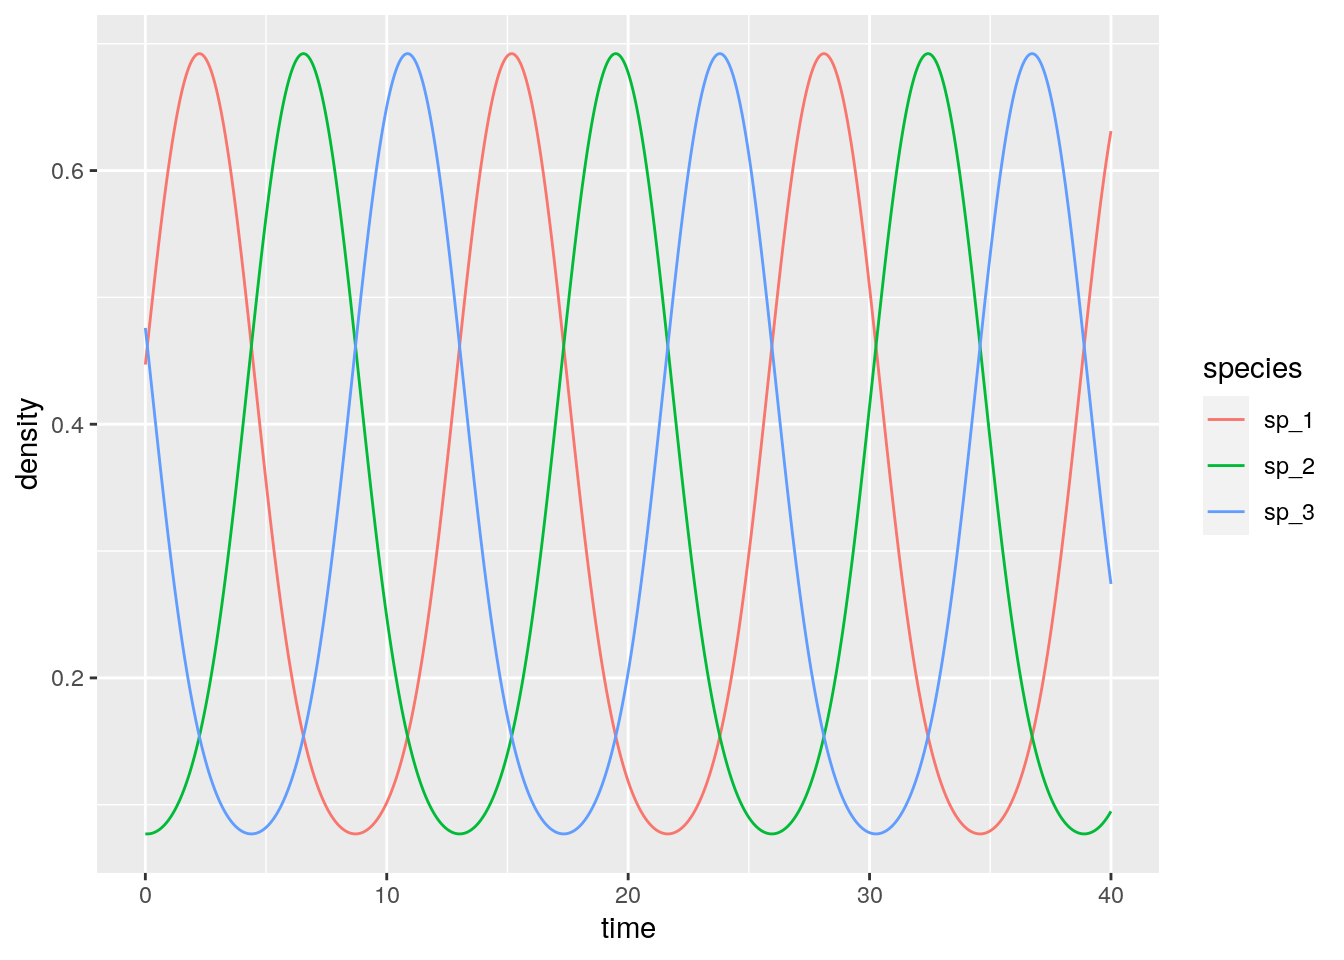
\includegraphics{A-Tour-of-the-Generalized-Lotka-Volterra-Model_files/figure-latex/refuctions-1} \end{center}

What if we start all populations at the same density?

\begin{Shaded}
\begin{Highlighting}[]
\NormalTok{x0 <-}\StringTok{ }\KeywordTok{rep}\NormalTok{(}\DecValTok{1} \OperatorTok{/}\StringTok{ }\DecValTok{3}\NormalTok{, }\DecValTok{3}\NormalTok{)}
\NormalTok{rps <-}\StringTok{ }\KeywordTok{integrate_RE}\NormalTok{(A, x0)}
\end{Highlighting}
\end{Shaded}

\begin{center}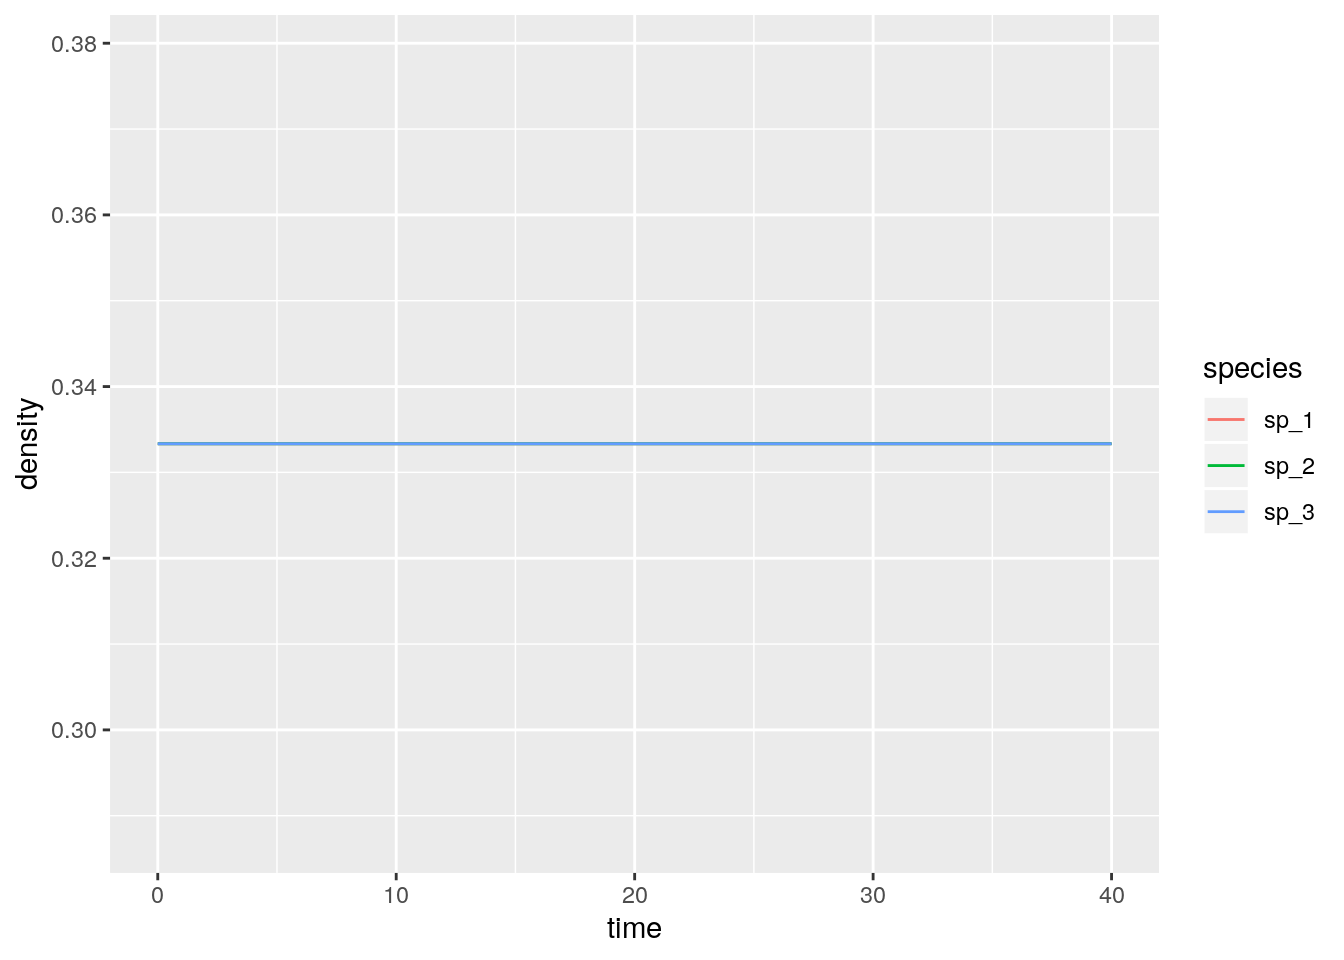
\includegraphics{A-Tour-of-the-Generalized-Lotka-Volterra-Model_files/figure-latex/rps2-1} \end{center}

And if they are close to the 1/3?

\begin{Shaded}
\begin{Highlighting}[]
\NormalTok{x0 <-}\StringTok{ }\KeywordTok{rep}\NormalTok{(}\DecValTok{1}\OperatorTok{/}\DecValTok{3}\NormalTok{, }\DecValTok{3}\NormalTok{) }\OperatorTok{+}\StringTok{ }\FloatTok{0.05} \OperatorTok{*}\StringTok{ }\KeywordTok{runif}\NormalTok{(}\DecValTok{3}\NormalTok{)}
\NormalTok{x0 <-}\StringTok{ }\NormalTok{x0 }\OperatorTok{/}\StringTok{ }\KeywordTok{sum}\NormalTok{(x0)}
\NormalTok{rps <-}\StringTok{ }\KeywordTok{integrate_RE}\NormalTok{(A, x0)}
\end{Highlighting}
\end{Shaded}

\begin{center}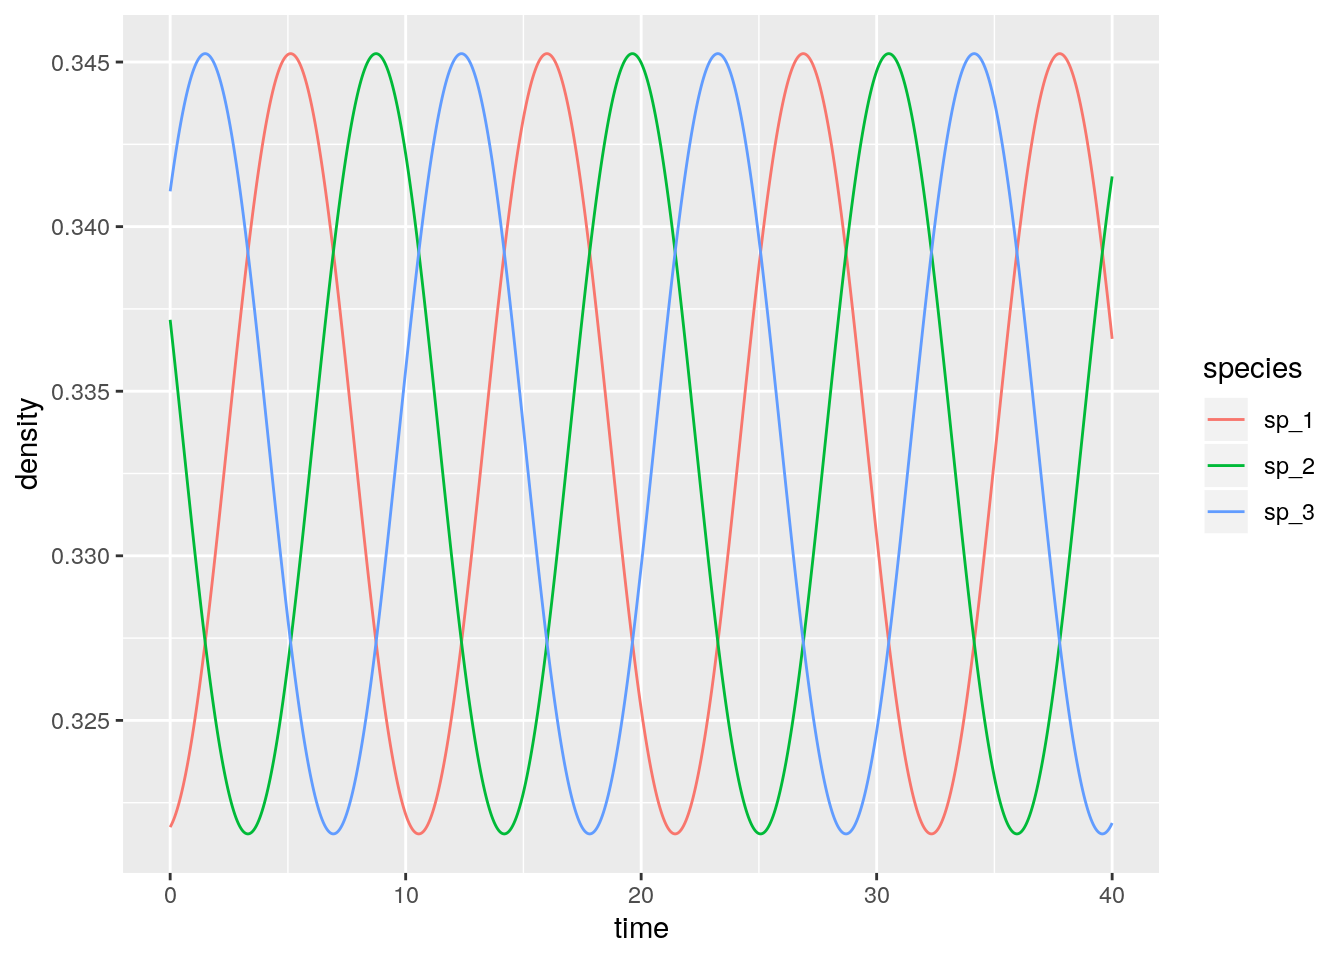
\includegraphics{A-Tour-of-the-Generalized-Lotka-Volterra-Model_files/figure-latex/rps3-1} \end{center}

\hypertarget{equivalence-with-glv}{%
\section{Equivalence with GLV}\label{equivalence-with-glv}}

For a given \(n-\)species GLV system, there is an equivalent \((n+1)-\)dimensional replicator equation with zeros in the last row of the matrix. To show this, let's take our functions for integrating GLV:

\begin{Shaded}
\begin{Highlighting}[]
\CommentTok{# Generalized Lotka-Volterra model}
\NormalTok{GLV <-}\StringTok{ }\ControlFlowTok{function}\NormalTok{(t, x, parameters)\{}
  \KeywordTok{with}\NormalTok{(}\KeywordTok{as.list}\NormalTok{(}\KeywordTok{c}\NormalTok{(x, parameters)), \{}
\NormalTok{    x[x }\OperatorTok{<}\StringTok{ }\DecValTok{10}\OperatorTok{^-}\DecValTok{8}\NormalTok{] <-}\StringTok{ }\DecValTok{0} \CommentTok{# prevent numerical problems}
\NormalTok{    dxdt <-}\StringTok{ }\NormalTok{x }\OperatorTok{*}\StringTok{ }\NormalTok{(r }\OperatorTok{+}\StringTok{ }\NormalTok{A }\OperatorTok\StringTok{ }\NormalTok{x)}
    \KeywordTok{list}\NormalTok{(dxdt)}
\NormalTok{  \})}
\NormalTok{\}}
\CommentTok{# general function to integrate GLV}
\NormalTok{integrate_GLV <-}\StringTok{ }\ControlFlowTok{function}\NormalTok{(r, A, x0, }\DataTypeTok{maxtime =} \DecValTok{100}\NormalTok{, }\DataTypeTok{steptime =} \FloatTok{0.5}\NormalTok{)\{}
\NormalTok{  times <-}\StringTok{ }\KeywordTok{seq}\NormalTok{(}\DecValTok{0}\NormalTok{, maxtime, }\DataTypeTok{by =}\NormalTok{ steptime)}
\NormalTok{  parameters <-}\StringTok{ }\KeywordTok{list}\NormalTok{(}\DataTypeTok{r =}\NormalTok{ r, }\DataTypeTok{A =}\NormalTok{ A)}
  \CommentTok{# solve numerically}
\NormalTok{  out <-}\StringTok{ }\KeywordTok{ode}\NormalTok{(}\DataTypeTok{y =}\NormalTok{ x0, }\DataTypeTok{times =}\NormalTok{ times, }
           \DataTypeTok{func =}\NormalTok{ GLV, }\DataTypeTok{parms =}\NormalTok{ parameters, }
           \DataTypeTok{method =} \StringTok{"ode45"}\NormalTok{)}
  \CommentTok{# plot and make into tidy form}
\NormalTok{  out <-}\StringTok{ }\KeywordTok{plot_ODE_output}\NormalTok{(out)}
  \KeywordTok{return}\NormalTok{(out)}
\NormalTok{\}}
\end{Highlighting}
\end{Shaded}

And integrate the simple system:

\begin{Shaded}
\begin{Highlighting}[]
\NormalTok{r <-}\StringTok{ }\KeywordTok{c}\NormalTok{(}\DecValTok{1}\NormalTok{, }\DecValTok{2}\NormalTok{, }\DecValTok{3}\NormalTok{)}
\NormalTok{A <-}\StringTok{ }\KeywordTok{matrix}\NormalTok{(}\KeywordTok{c}\NormalTok{(}\OperatorTok{-}\DecValTok{1}\NormalTok{, }\FloatTok{0.5}\NormalTok{, }\FloatTok{0.1}\NormalTok{,}
              \FloatTok{-0.7}\NormalTok{, }\DecValTok{-2}\NormalTok{, }\DecValTok{0}\NormalTok{,}
              \FloatTok{-0.3}\NormalTok{, }\DecValTok{0}\NormalTok{, }\DecValTok{-5}\NormalTok{), }\DecValTok{3}\NormalTok{, }\DecValTok{3}\NormalTok{, }\DataTypeTok{byrow =} \OtherTok{TRUE}\NormalTok{)}
\NormalTok{x0 <-}\StringTok{ }\KeywordTok{c}\NormalTok{(}\FloatTok{0.1}\NormalTok{, }\DecValTok{3}\NormalTok{, }\DecValTok{1}\NormalTok{)}
\NormalTok{glvex <-}\StringTok{ }\KeywordTok{integrate_GLV}\NormalTok{(r, A, x0)}
\end{Highlighting}
\end{Shaded}

\begin{center}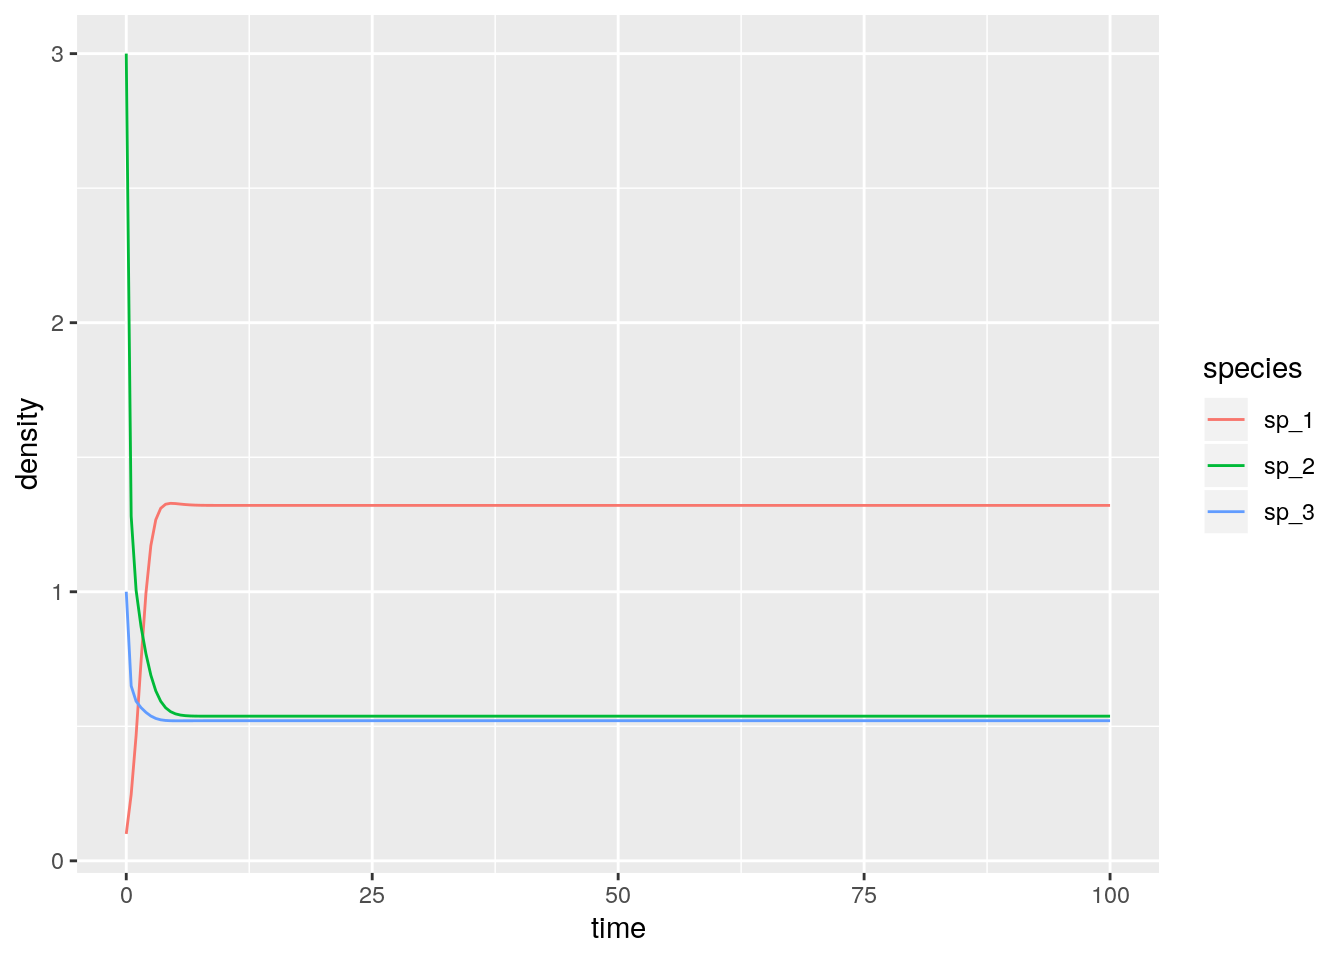
\includegraphics{A-Tour-of-the-Generalized-Lotka-Volterra-Model_files/figure-latex/exampleglvtore1-1} \end{center}

And now build an equivalent RE system. Form a matrix \(B\) with the matrix \(A\) in the first \(n\) rows and columns, and the vector \(r\) as the \((n+1)\)th column:

\begin{Shaded}
\begin{Highlighting}[]
\NormalTok{B <-}\StringTok{ }\KeywordTok{matrix}\NormalTok{(}\DecValTok{0}\NormalTok{, }\DecValTok{4}\NormalTok{, }\DecValTok{4}\NormalTok{)}
\NormalTok{B[}\DecValTok{1}\OperatorTok{:}\DecValTok{3}\NormalTok{, }\DecValTok{1}\OperatorTok{:}\DecValTok{3}\NormalTok{] <-}\StringTok{ }\NormalTok{A}
\NormalTok{B[}\DecValTok{1}\OperatorTok{:}\DecValTok{3}\NormalTok{, }\DecValTok{4}\NormalTok{] <-}\StringTok{ }\NormalTok{r}
\NormalTok{B}
\NormalTok{y0 <-}\StringTok{ }\KeywordTok{c}\NormalTok{(x0, }\DecValTok{1}\NormalTok{)}
\NormalTok{y0 <-}\StringTok{ }\NormalTok{y0 }\OperatorTok{/}\StringTok{ }\KeywordTok{sum}\NormalTok{(y0)}
\NormalTok{reex <-}\StringTok{ }\KeywordTok{integrate_RE}\NormalTok{(B, y0)}
\end{Highlighting}
\end{Shaded}

\begin{center}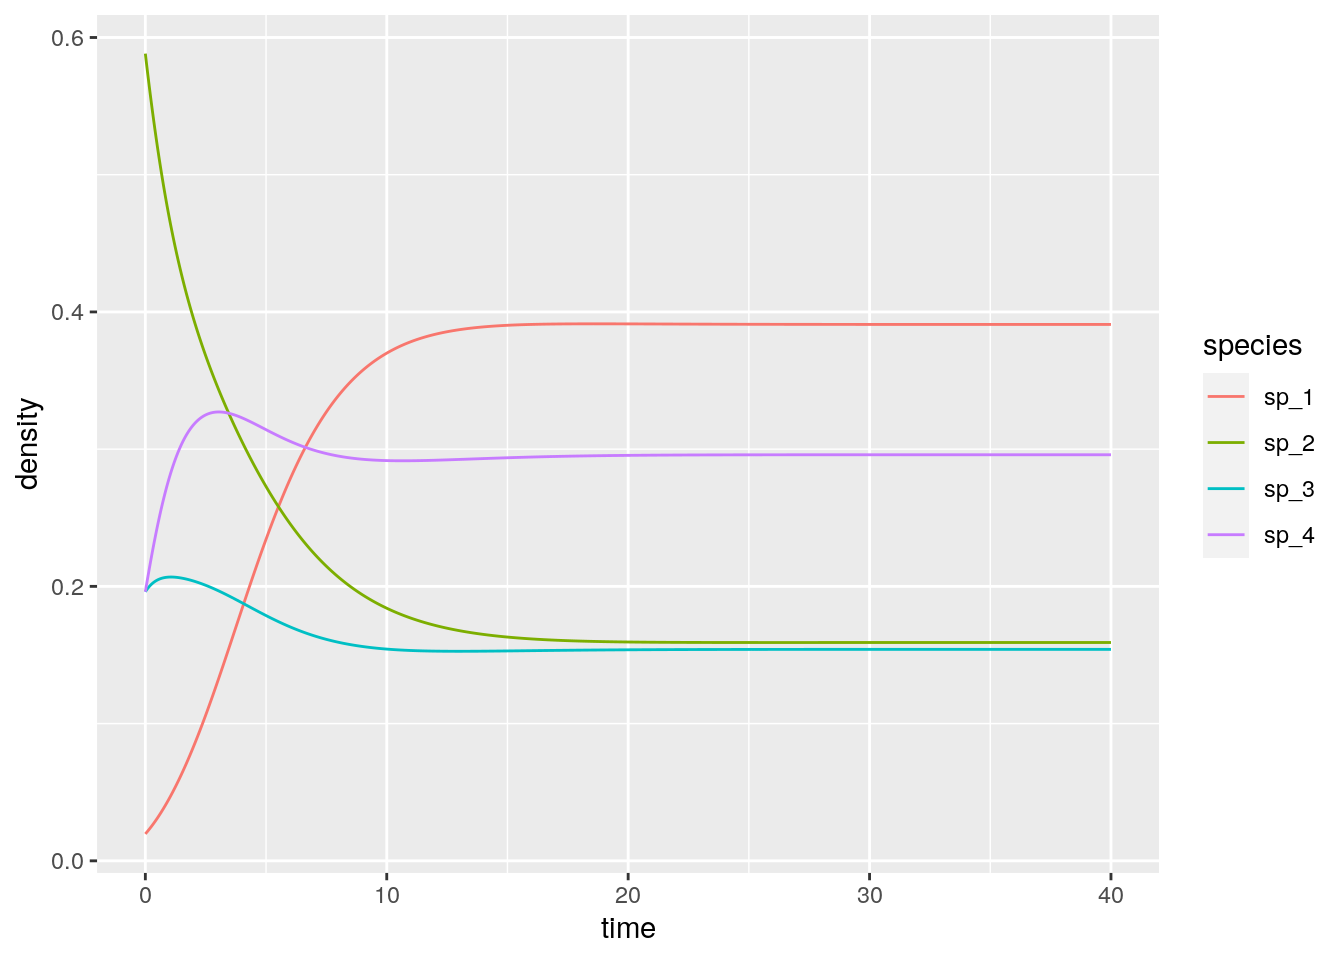
\includegraphics{A-Tour-of-the-Generalized-Lotka-Volterra-Model_files/figure-latex/redynamicsfromglv-1} \end{center}

\begin{verbatim}
#      [,1] [,2] [,3] [,4]
# [1,] -1.0  0.5  0.1    1
# [2,] -0.7 -2.0  0.0    2
# [3,] -0.3  0.0 -5.0    3
# [4,]  0.0  0.0  0.0    0
\end{verbatim}

Now let's look at the equilibrium of the GLV model:

\begin{Shaded}
\begin{Highlighting}[]
\NormalTok{glvex }\OperatorTok\StringTok{ }\KeywordTok{filter}\NormalTok{(time }\OperatorTok{==}\StringTok{ }\DecValTok{100}\NormalTok{)}
\end{Highlighting}
\end{Shaded}

\begin{verbatim}
# # A tibble: 3 x 3
#    time species density
#   <dbl> <chr>     <dbl>
# 1   100 sp_1      1.32 
# 2   100 sp_2      0.538
# 3   100 sp_3      0.521
\end{verbatim}

And recover it from the RE equation (just divide by the density of the extra ``species''):

\begin{Shaded}
\begin{Highlighting}[]
\NormalTok{reex }\OperatorTok\StringTok{ }\KeywordTok{filter}\NormalTok{(time }\OperatorTok{==}\StringTok{ }\DecValTok{40}\NormalTok{)}
\NormalTok{reex }\OperatorTok\StringTok{ }\KeywordTok{filter}\NormalTok{(time }\OperatorTok{==}\StringTok{ }\DecValTok{40}\NormalTok{) }\OperatorTok\StringTok{ }\KeywordTok{mutate}\NormalTok{(}\DataTypeTok{density =}\NormalTok{ density }\OperatorTok{/}\StringTok{ }\KeywordTok{tail}\NormalTok{(density, }\DecValTok{1}\NormalTok{))}
\end{Highlighting}
\end{Shaded}

\begin{verbatim}
# # A tibble: 4 x 3
#    time species density
#   <dbl> <chr>     <dbl>
# 1    40 sp_1      0.391
# 2    40 sp_2      0.159
# 3    40 sp_3      0.154
# 4    40 sp_4      0.296
# # A tibble: 4 x 3
#    time species density
#   <dbl> <chr>     <dbl>
# 1    40 sp_1      1.32 
# 2    40 sp_2      0.538
# 3    40 sp_3      0.521
# 4    40 sp_4      1
\end{verbatim}

Not only the equilibria are the same, but also the dynamics are the same once time has been properly rescaled. Similarly, for each RE system we can always recover a matrix with zero in the last row by applying the transformations detailed above, and therefore recover the corresponding GLV. For example, take the matrix for the RPS above, and make each coefficient in the last row zero by adding the appropriate constant to each column. Then one recovers some sort of a predator-prey system:

\begin{Shaded}
\begin{Highlighting}[]
\NormalTok{r <-}\StringTok{ }\KeywordTok{c}\NormalTok{(}\OperatorTok{-}\DecValTok{1}\NormalTok{, }\DecValTok{1}\NormalTok{)}
\NormalTok{A <-}\StringTok{ }\KeywordTok{matrix}\NormalTok{(}\KeywordTok{c}\NormalTok{(}\OperatorTok{-}\DecValTok{1}\NormalTok{, }\DecValTok{2}\NormalTok{,}
              \DecValTok{-2}\NormalTok{, }\DecValTok{1}\NormalTok{), }\DecValTok{2}\NormalTok{, }\DecValTok{2}\NormalTok{, }\DataTypeTok{byrow =} \OtherTok{TRUE}\NormalTok{)}
\NormalTok{x0 <-}\StringTok{ }\KeywordTok{c}\NormalTok{(}\FloatTok{0.9}\NormalTok{, }\FloatTok{1.1}\NormalTok{)}
\NormalTok{glvex <-}\StringTok{ }\KeywordTok{integrate_GLV}\NormalTok{(r, A, x0, }\DataTypeTok{maxtime =} \DecValTok{15}\NormalTok{, }\DataTypeTok{steptime =} \FloatTok{0.01}\NormalTok{)}
\end{Highlighting}
\end{Shaded}

\begin{center}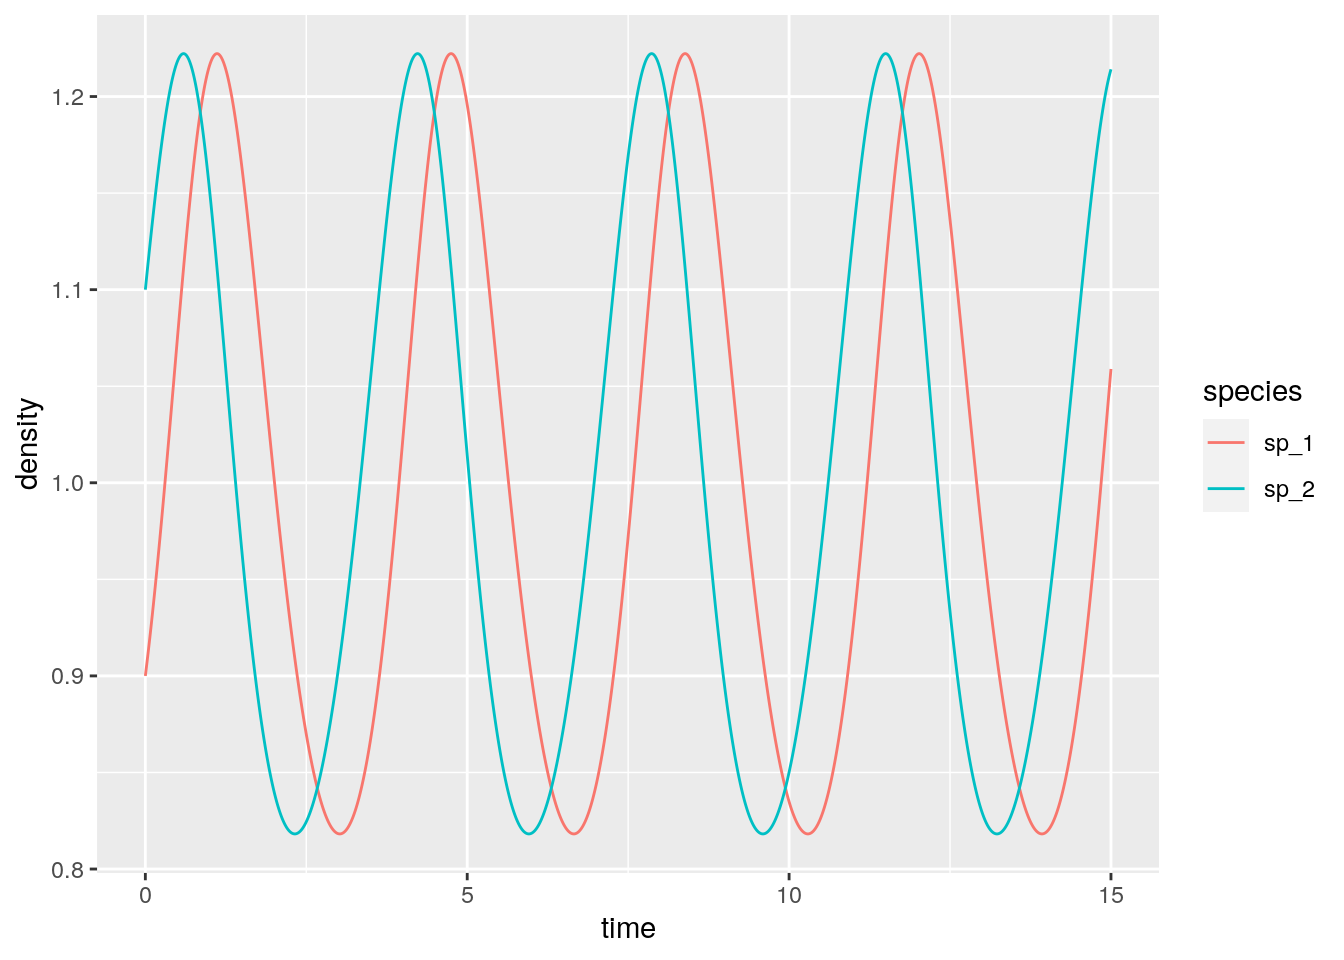
\includegraphics{A-Tour-of-the-Generalized-Lotka-Volterra-Model_files/figure-latex/exampleretoglv1-1} \end{center}

in which the species oscillate around one.

\hypertarget{hypertournament-games}{%
\subsection{Hypertournament games}\label{hypertournament-games}}

The rock-paper-scissor game above is a simple case of a ``hypertournament'' game. Take the zero-sum payoff matrix \(A = -A^t\). Then, we have

\[
\sum_i \sum_j A_{ij} x_i x_j = 0
\]
and the RE simplifies to

\[
\dfrac{d x}{dt} = D(x) A x
\]

At equilibrium, either some elements of \(x\) are zero, or

\[
A x^\star = 0
\]
meaning that if a feasible equilibrium \(x^\star\) exists, it is an eigenvector of \(A\) corresponding to a zero eigenvalue.

\hypertarget{number-of-coexisting-species}{%
\subsubsection{Number of coexisting species}\label{number-of-coexisting-species}}

We now show how the equations above can arise when modeling ecological dynamics. Suppose that a forest is composed of a fixed number of trees. Each time a tree dies (with rate \(d = 1\) for all species), a gap in the canopy opens, and species will compete to colonize it. Let's assume that two seeds (sampled with probability proportional to the density of the species) land in the empty patch, and that they compete to fill the gap. Call \(H_{ij}\) the probability that \(i\) wins when competing with \(j\); we have \(H_{ij} + H_{ji} = 1\). We can write the dynamics \citep{grilli2017higher} as:

\[
\begin{aligned}
  \dfrac{d x}{dt} &= x_i \left(\sum_j 2 H_{ij} x_j - 1 \right) \\
  &=x_i \sum_j (2 H_{ij} x_j - x_j) \\
  &= x_i \sum_j (H_{ij} x_j  + (1 - H_{ji}) x_j - x_j) \\
  &= x_i \sum_j (H_{ij} - H_{ji}) x_j \\
  &= x_i  \sum_j A_{ij} x_j
\end{aligned}
\]

I.e., we recover the RE for a zero-sum game. What happens if we draw \(H\) (and therefore \(A\)) at random? \citet{allesina2011competitive} and \citet{grilli2017higher} applied the results of \citet{fisher1995optimal} and \citet{brandl2017distribution} to show that, when \(n\) species compete, the probability of observing \(k\) coexisting is \(p(k|n) = \binom{n}{k} 2^{1-n}\) when \(k\) is odd, and \(p(k|n) = 0\) when \(k\) is even.

Importantly, to find the set of coexisting species we do not need to integrate dynamics. One can use linear programming to solve for the set of species that will coexist.

\begin{Shaded}
\begin{Highlighting}[]
\KeywordTok{library}\NormalTok{(lpSolve)}
\CommentTok{# Build a random matrix H such that H_ij + H_ji = 1}
\NormalTok{random_H <-}\StringTok{ }\ControlFlowTok{function}\NormalTok{(n)\{}
  \CommentTok{# build random hypertournament H}
\NormalTok{  H <-}\StringTok{ }\KeywordTok{matrix}\NormalTok{(}\KeywordTok{runif}\NormalTok{(n }\OperatorTok{*}\StringTok{ }\NormalTok{n), n, n)}
  \KeywordTok{return}\NormalTok{(H }\OperatorTok{/}\StringTok{ }\NormalTok{(H }\OperatorTok{+}\StringTok{ }\KeywordTok{t}\NormalTok{(H)))}
\NormalTok{\}}
\CommentTok{# Find the optimal strategy for the two-person game encoded in H}
\CommentTok{# using linear programming.}
\CommentTok{# This is also the coexistence equilibrium of the dynamical system.}
\NormalTok{find_optimal_strategy <-}\StringTok{ }\ControlFlowTok{function}\NormalTok{(H)\{}
\NormalTok{  n <-}\StringTok{ }\KeywordTok{dim}\NormalTok{(H)[}\DecValTok{1}\NormalTok{]}
\NormalTok{  f.obj <-}\StringTok{ }\KeywordTok{rep}\NormalTok{(}\DecValTok{1}\NormalTok{, n)}
\NormalTok{  f.con <-}\StringTok{ }\NormalTok{H}
\NormalTok{  f.rhs <-}\StringTok{ }\KeywordTok{rep}\NormalTok{(}\DecValTok{1}\NormalTok{, n)}
\NormalTok{  f.dir <-}\StringTok{ }\KeywordTok{rep}\NormalTok{(}\StringTok{"<="}\NormalTok{, n)}
\NormalTok{  z <-}\StringTok{ }\KeywordTok{lp}\NormalTok{ (}\StringTok{"max"}\NormalTok{, f.obj, f.con, f.dir, f.rhs)}
  \KeywordTok{return}\NormalTok{(z}\OperatorTok{$}\NormalTok{solution }\OperatorTok{/}\StringTok{ }\KeywordTok{sum}\NormalTok{(z}\OperatorTok{$}\NormalTok{solution))}
\NormalTok{\}}
\end{Highlighting}
\end{Shaded}

Now let's try to count how many species suvive when starting with 10:

\begin{Shaded}
\begin{Highlighting}[]
\NormalTok{n <-}\StringTok{ }\DecValTok{10}
\NormalTok{num_simulations <-}\StringTok{ }\DecValTok{5000}
\NormalTok{results <-}\StringTok{ }\KeywordTok{tibble}\NormalTok{(}\DataTypeTok{simulation =} \DecValTok{1}\OperatorTok{:}\NormalTok{num_simulations, }\DataTypeTok{coexisting =} \OtherTok{NA}\NormalTok{)}
\ControlFlowTok{for}\NormalTok{ (i }\ControlFlowTok{in} \DecValTok{1}\OperatorTok{:}\NormalTok{num_simulations)\{}
\NormalTok{  H <-}\StringTok{ }\KeywordTok{random_H}\NormalTok{(n)}
\NormalTok{  coexisting <-}\StringTok{ }\KeywordTok{find_optimal_strategy}\NormalTok{(H)}
\NormalTok{  results[i,}\StringTok{"coexisting"}\NormalTok{] <-}\StringTok{ }\KeywordTok{sum}\NormalTok{(coexisting }\OperatorTok{>}\StringTok{ }\DecValTok{0}\NormalTok{)}
\NormalTok{\}}
\CommentTok{# and plot}
\KeywordTok{ggplot}\NormalTok{(}\DataTypeTok{data =}\NormalTok{ results) }\OperatorTok{+}\StringTok{ }\KeywordTok{aes}\NormalTok{(}\DataTypeTok{x =}\NormalTok{ coexisting) }\OperatorTok{+}\StringTok{ }\KeywordTok{geom_bar}\NormalTok{() }\OperatorTok{+}\StringTok{ }\KeywordTok{scale_x_continuous}\NormalTok{(}\DataTypeTok{breaks =} \DecValTok{0}\OperatorTok{:}\DecValTok{10}\NormalTok{)}
\end{Highlighting}
\end{Shaded}

\begin{center}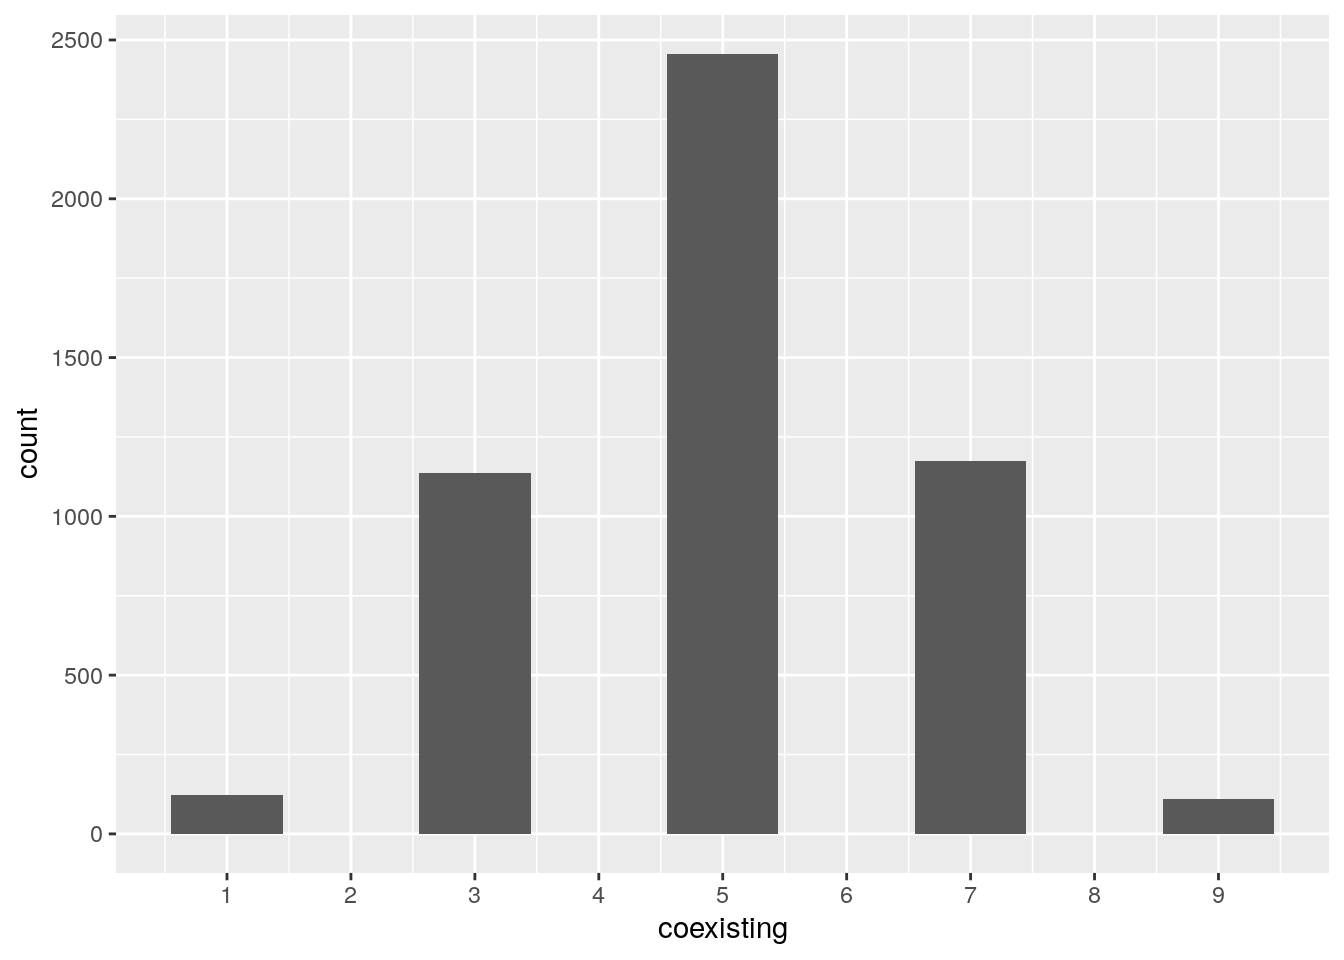
\includegraphics{A-Tour-of-the-Generalized-Lotka-Volterra-Model_files/figure-latex/coexistlphist-1} \end{center}

\hypertarget{lyapunov-function}{%
\subsection{Lyapunov function}\label{lyapunov-function}}

In the rock-paper-scissor example above, species cycled neutrally around the unique equilibrium point. To show that this is in fact the behavior of this type of RE, we write a Lyapunov function. By finding a constant of motion we can show that the species will follow closed orbits.

Suppose \(x_{i}^\star > 0\) is the equilibrium for the system. We write:

\[
V(x) = -\sum_i x_i^\ast \log \frac{x_i}{x_i^\ast} .
\]

Because of Gibbs' inequality, \(V(x) \geq 0\) for any \(x\), and is equal to zero only if \(x = x^\star\). Note also that at equilibrium \(2 \sum_j H_{ij} x_j^\star = 1\). We write:

\[
\begin{aligned}
  \dfrac{d V}{d t} &= \sum_i \dfrac{\partial V}{\partial x_i}
  \dfrac{d x_i}{d t}\\
  &= - \sum_i \frac{x_i^\star}{x_i} \dfrac{d x_i}{d t} \\
  &= -2 \sum_{i,j} x_i^\star H_{ij}x_j + \sum_i x_i^\star\\
  &= -2 \sum_{i,j} x_i^\star H_{ij}x_j + 1\\
  &= \sum_j \left(-2 \sum_i H_{ij}x_i^\star \right) x_j + 1\\
  &= \sum_j \left(-2 \sum_i (1 - H_{ji}) x_i^\star \right) x_j + 1\\
  &= \sum_j \left(-2 \sum_i x_i^\star + 2 \sum_i H_{ji} x_i^\star \right) x_j
  + 1 \\
  &= \sum_j \left(-2 + 1 \right) x_j  + 1 \\
  &=- \sum_j x_j + 1\\
  &= 0 
\end{aligned}
\]

We have found a constant of motion, meaning that the system will follow closed orbits. Hence, unless we start the system precisely at \(x^\ast\), the abundances will cycle neutrally around the equilibrium.

Let's try with a larger system:

\begin{Shaded}
\begin{Highlighting}[]
\NormalTok{n <-}\StringTok{ }\DecValTok{5}
\CommentTok{# search for random H yielding all species coexisting}
\NormalTok{i <-}\StringTok{ }\DecValTok{0}
\ControlFlowTok{while}\NormalTok{(}\OtherTok{TRUE}\NormalTok{)\{}
\NormalTok{  i <-}\StringTok{ }\NormalTok{i }\OperatorTok{+}\StringTok{ }\DecValTok{1}
  \KeywordTok{set.seed}\NormalTok{(i)}
\NormalTok{  H <-}\StringTok{ }\KeywordTok{random_H}\NormalTok{(n)}
\NormalTok{  x_star <-}\StringTok{ }\KeywordTok{find_optimal_strategy}\NormalTok{(H)}
  \ControlFlowTok{if}\NormalTok{ (}\KeywordTok{all}\NormalTok{(x_star) }\OperatorTok{>}\StringTok{ }\DecValTok{0}\NormalTok{) }\ControlFlowTok{break}
\NormalTok{\}}
\CommentTok{# payoff matrix}
\NormalTok{A <-}\StringTok{ }\NormalTok{H }\OperatorTok{-}\StringTok{ }\KeywordTok{t}\NormalTok{(H)}
\CommentTok{# initial conditions close to equilibrium}
\NormalTok{x0 <-}\StringTok{ }\NormalTok{x_star }\OperatorTok{+}\StringTok{ }\KeywordTok{runif}\NormalTok{(n) }\OperatorTok{*}\StringTok{ }\FloatTok{0.2}
\NormalTok{x0 <-}\StringTok{ }\NormalTok{x0 }\OperatorTok{/}\StringTok{ }\KeywordTok{sum}\NormalTok{(x0)}
\NormalTok{fivespp <-}\StringTok{ }\KeywordTok{integrate_RE}\NormalTok{(A, x0, }\DataTypeTok{maxtime =} \DecValTok{400}\NormalTok{, }\DataTypeTok{steptime =} \FloatTok{0.1}\NormalTok{)}
\end{Highlighting}
\end{Shaded}

\begin{center}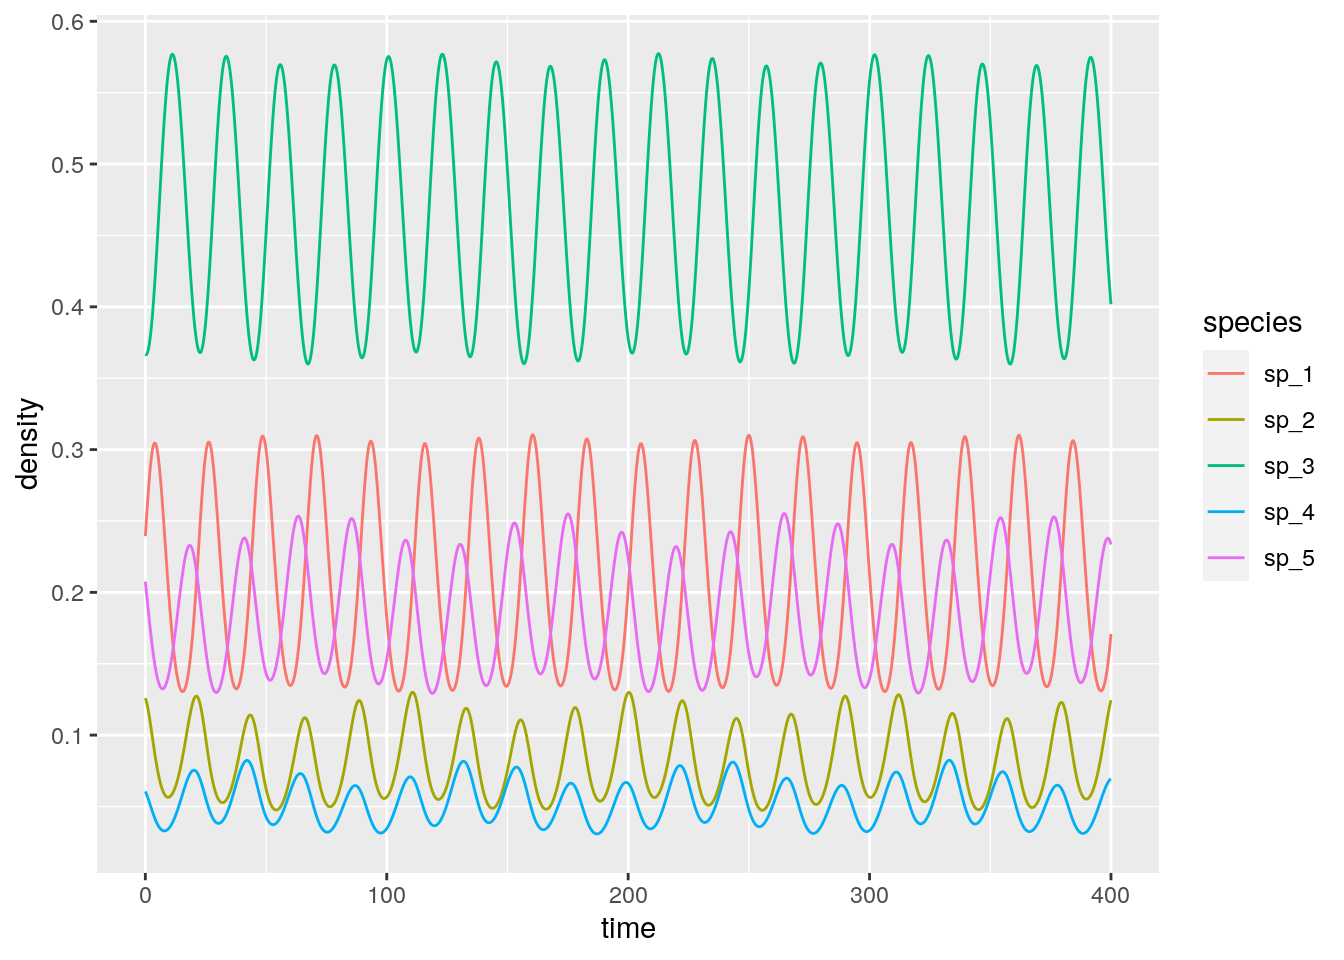
\includegraphics{A-Tour-of-the-Generalized-Lotka-Volterra-Model_files/figure-latex/reneutral-1} \end{center}

\hypertarget{higher-order-interactions}{%
\subsection{Higher-order interactions}\label{higher-order-interactions}}

We can extend the game above to the case in which three (or more) seeds compete to fill each patch. \citet{grilli2017higher} showed that in this case, one can write the replicator equation:

\[
\dfrac{d x_i}{dt} = x_i \sum_{j,k} A_{ijk} x_j x_k
\]
where the tensor \(A\) (a three-dimensional matrix) encodes the effect of a pair of species (\(j\) and \(k\)) on the density of \(i\). Importantly, one can choose the tensor such that the equilibrium is the same as for the two-player replicator equation: take \(A_{ijk} = 2 H_{ij} H_{ik} - H_{ji} H_{jk} - H_{ki} H_{kj}\), which can be derived from first principles by writing the stochastic dynamics. What is surprising is that, while the equilibrium is unchanged, the dynamics are now globally stable:

\begin{Shaded}
\begin{Highlighting}[]
\CommentTok{# Now payoff is a tensor}
\NormalTok{RE_}\DecValTok{3}\NormalTok{ <-}\StringTok{ }\ControlFlowTok{function}\NormalTok{(t, x, parameters)\{}
  \KeywordTok{with}\NormalTok{(}\KeywordTok{as.list}\NormalTok{(}\KeywordTok{c}\NormalTok{(x, parameters)), \{}
\NormalTok{    x[x }\OperatorTok{<}\StringTok{ }\DecValTok{10}\OperatorTok{^-}\DecValTok{8}\NormalTok{] <-}\StringTok{ }\DecValTok{0} \CommentTok{# prevent numerical problems}
\NormalTok{    x <-}\StringTok{ }\NormalTok{x }\OperatorTok{/}\StringTok{ }\KeywordTok{sum}\NormalTok{(x) }\CommentTok{# keep on simplex}
\NormalTok{    n <-}\StringTok{ }\KeywordTok{length}\NormalTok{(x)}
\NormalTok{    dxidt <-}\StringTok{ }\KeywordTok{rep}\NormalTok{(}\DecValTok{0}\NormalTok{, n)}
    \ControlFlowTok{for}\NormalTok{ (i }\ControlFlowTok{in} \DecValTok{1}\OperatorTok{:}\NormalTok{n)\{}
\NormalTok{      dxidt[i] <-}\StringTok{ }\NormalTok{x[i] }\OperatorTok{*}\StringTok{ }\NormalTok{x }\OperatorTok\StringTok{ }\NormalTok{P3[i,,] }\OperatorTok\StringTok{ }\NormalTok{x}
\NormalTok{    \}}
    \KeywordTok{list}\NormalTok{(dxidt)}
\NormalTok{  \})}
\NormalTok{\}}
\CommentTok{# general function to integrate RE_3}
\NormalTok{integrate_RE_}\DecValTok{3}\NormalTok{ <-}\StringTok{ }\ControlFlowTok{function}\NormalTok{(H, x0, }\DataTypeTok{maxtime =} \DecValTok{40}\NormalTok{, }\DataTypeTok{steptime =} \FloatTok{0.05}\NormalTok{)\{}
\NormalTok{  times <-}\StringTok{ }\KeywordTok{seq}\NormalTok{(}\DecValTok{0}\NormalTok{, maxtime, }\DataTypeTok{by =}\NormalTok{ steptime)}
\NormalTok{  n <-}\StringTok{ }\KeywordTok{nrow}\NormalTok{(H)}
\NormalTok{  P3 <-}\StringTok{ }\KeywordTok{array}\NormalTok{(}\DecValTok{0}\NormalTok{, }\KeywordTok{c}\NormalTok{(n, n, n))}
  \ControlFlowTok{for}\NormalTok{ (i }\ControlFlowTok{in} \DecValTok{1}\OperatorTok{:}\NormalTok{n)\{}
    \ControlFlowTok{for}\NormalTok{ (j }\ControlFlowTok{in} \DecValTok{1}\OperatorTok{:}\NormalTok{n)\{}
      \ControlFlowTok{for}\NormalTok{ (k }\ControlFlowTok{in} \DecValTok{1}\OperatorTok{:}\NormalTok{n)\{}
\NormalTok{        P3[i,j,k] <-}\StringTok{ }\DecValTok{2} \OperatorTok{*}\StringTok{ }\NormalTok{H[i,j] }\OperatorTok{*}\StringTok{ }\NormalTok{H[i,k] }\OperatorTok{-}\StringTok{  }\NormalTok{H[j,i] }\OperatorTok{*}\StringTok{ }\NormalTok{H[j,k] }\OperatorTok{-}\StringTok{ }\NormalTok{H[k,i] }\OperatorTok{*}\StringTok{ }\NormalTok{H[k,j]}
\NormalTok{      \}}
\NormalTok{    \}}
\NormalTok{  \}}
\NormalTok{  parameters <-}\StringTok{ }\KeywordTok{list}\NormalTok{(}\DataTypeTok{P3 =}\NormalTok{ P3)}
  \CommentTok{# solve numerically}
\NormalTok{  out <-}\StringTok{ }\KeywordTok{ode}\NormalTok{(}\DataTypeTok{y =}\NormalTok{ x0, }\DataTypeTok{times =}\NormalTok{ times, }
           \DataTypeTok{func =}\NormalTok{ RE_}\DecValTok{3}\NormalTok{, }\DataTypeTok{parms =}\NormalTok{ parameters, }
           \DataTypeTok{method =} \StringTok{"ode45"}\NormalTok{)}
  \CommentTok{# plot and make into tidy form}
\NormalTok{  out <-}\StringTok{ }\KeywordTok{plot_ODE_output}\NormalTok{(out)}
  \KeywordTok{return}\NormalTok{(out)}
\NormalTok{\}}
\CommentTok{# integrate the system above}
\NormalTok{fivespp <-}\StringTok{ }\KeywordTok{integrate_RE_3}\NormalTok{(H, x0, }\DataTypeTok{maxtime =} \DecValTok{800}\NormalTok{, }\DataTypeTok{steptime =} \FloatTok{0.1}\NormalTok{)}
\end{Highlighting}
\end{Shaded}

\begin{center}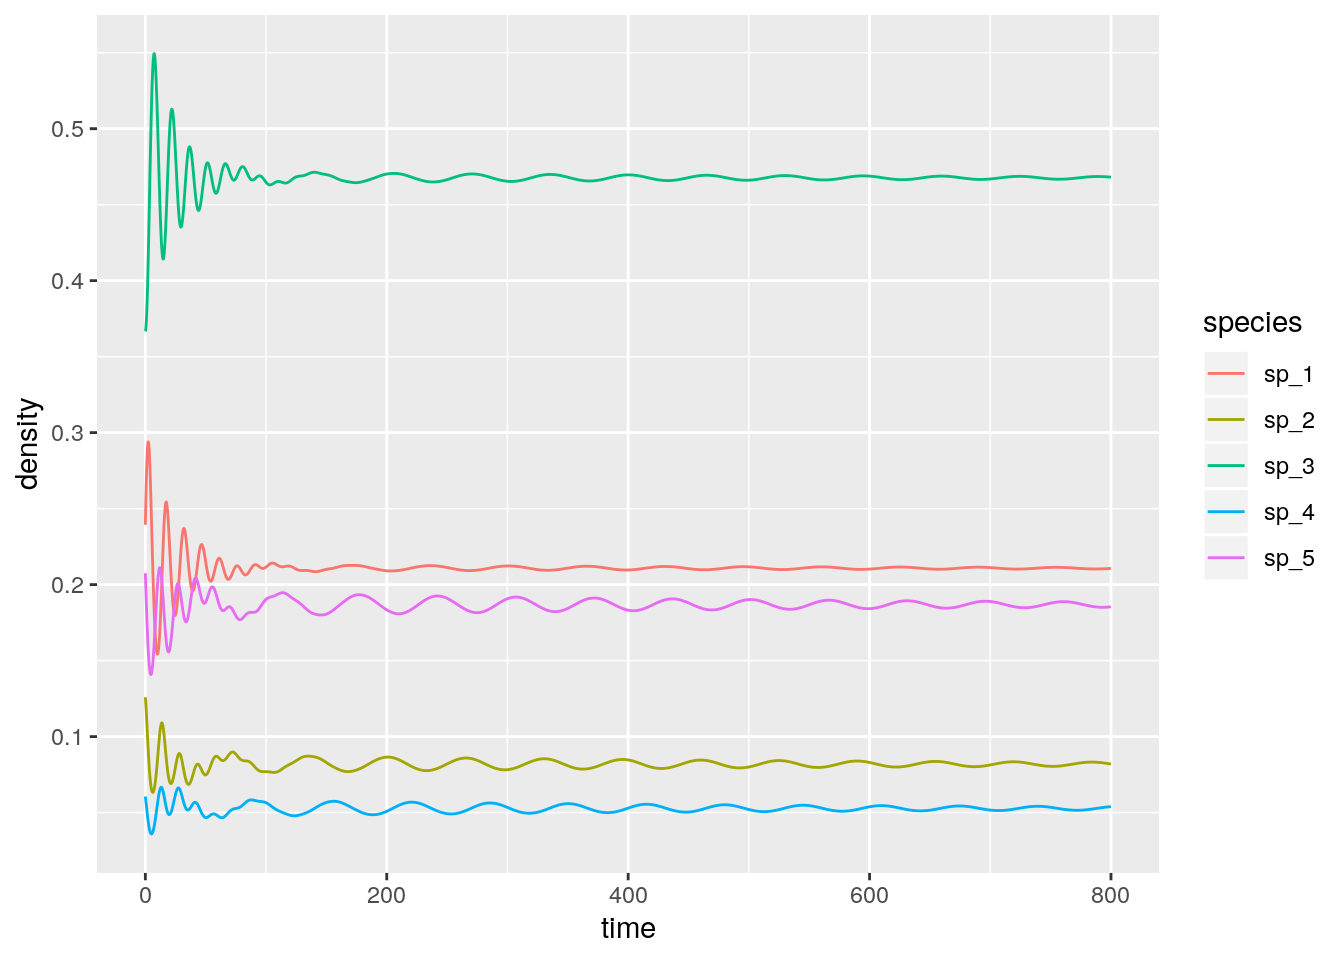
\includegraphics{A-Tour-of-the-Generalized-Lotka-Volterra-Model_files/figure-latex/rehoi-1} \end{center}

And the rock-paper-scissors:

\begin{Shaded}
\begin{Highlighting}[]
\NormalTok{H <-}\StringTok{ }\KeywordTok{matrix}\NormalTok{(}\KeywordTok{c}\NormalTok{(}\DecValTok{1}\OperatorTok{/}\DecValTok{2}\NormalTok{, }\DecValTok{1}\NormalTok{, }\DecValTok{0}\NormalTok{,}
              \DecValTok{0}\NormalTok{, }\DecValTok{1}\OperatorTok{/}\DecValTok{2}\NormalTok{, }\DecValTok{1}\NormalTok{,}
              \DecValTok{1}\NormalTok{, }\DecValTok{0}\NormalTok{, }\DecValTok{1}\OperatorTok{/}\DecValTok{2}\NormalTok{), }\DecValTok{3}\NormalTok{, }\DecValTok{3}\NormalTok{, }\DataTypeTok{byrow =} \OtherTok{TRUE}\NormalTok{)}
\NormalTok{x0 <-}\StringTok{ }\KeywordTok{runif}\NormalTok{(}\DecValTok{3}\NormalTok{)}
\NormalTok{x0 <-}\StringTok{ }\NormalTok{x0 }\OperatorTok{/}\StringTok{ }\KeywordTok{sum}\NormalTok{(x0)}
\NormalTok{rps <-}\StringTok{ }\KeywordTok{integrate_RE_3}\NormalTok{(H, x0, }\DataTypeTok{maxtime =} \DecValTok{50}\NormalTok{, }\DataTypeTok{steptime =} \FloatTok{0.1}\NormalTok{)}
\end{Highlighting}
\end{Shaded}

\begin{center}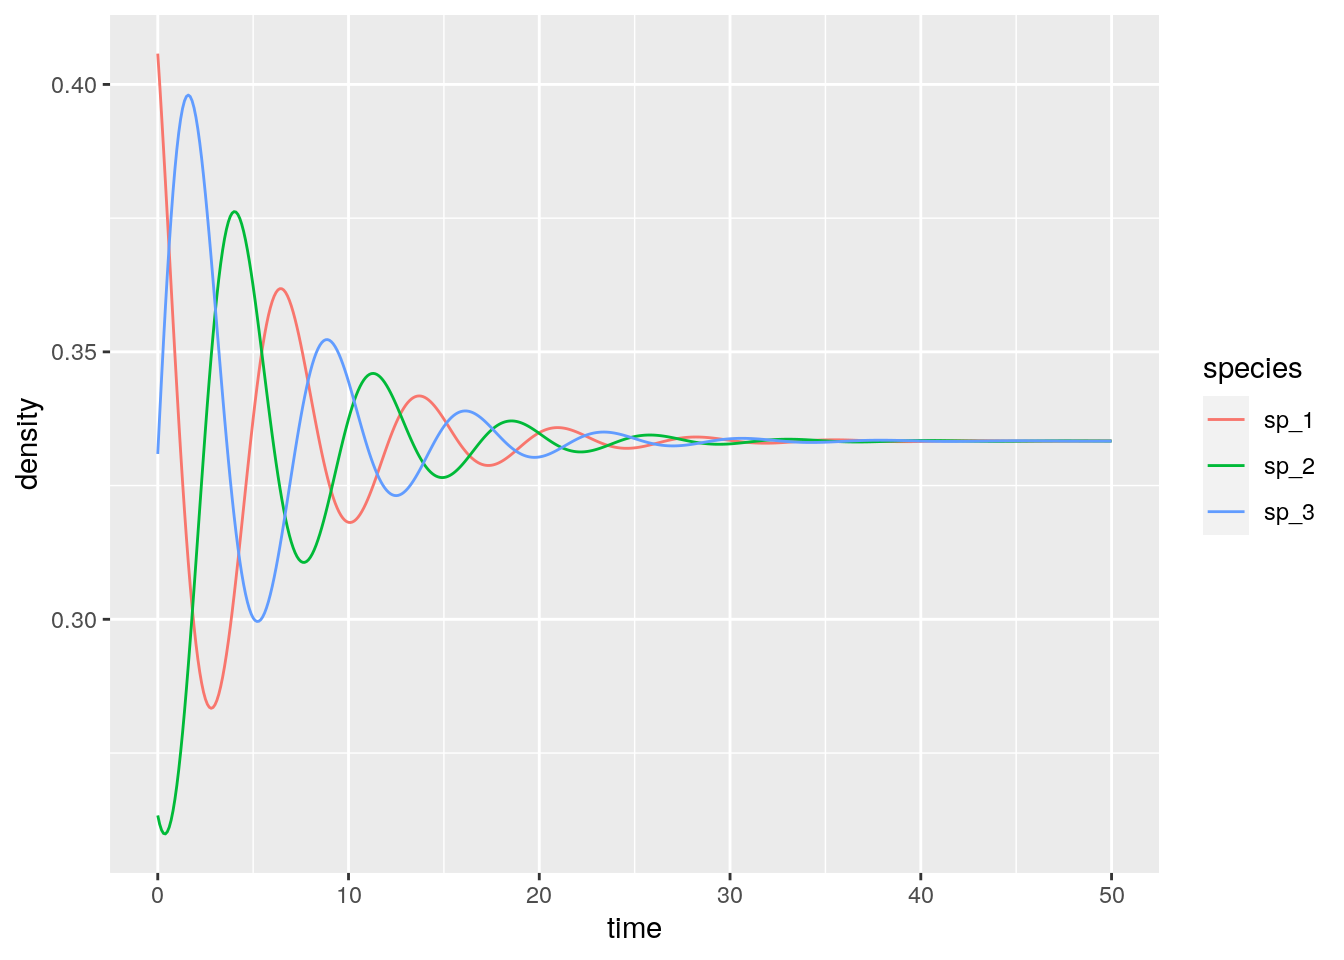
\includegraphics{A-Tour-of-the-Generalized-Lotka-Volterra-Model_files/figure-latex/rpshoi-1} \end{center}

\hypertarget{data}{%
\chapter{Simple models for synthetic communities}\label{data}}

Ecologists have performed large experiments in which different assemblages of species are co-cultured. These experiments have been conducted with plants (for example, Biodiversity Ecosystem Functioning experiments e.g., \citep{hector1999plant} \citep{tilman2001diversity} \citep{cadotte2013experimental}) and in the laboratory using protozoan, algae or bacteria. Two commonly-encountered problems in this type of experiments have to to with the scaling of the number of experiments with the number of species, and with the probability of coexistence.

\textbf{Scale:} How many communities can we form from a pool of \(n\) species? We can culture a single species in isolation (\(n\) possibilities), two species in pair (\(n(n-1) / 2\) possibilities), and so on. The total is therefore:

\[
\sum_{j=1}^n \binom{n}{j} = 2^n -1
\]

And this is only considering the presence/absence of each species! Moreover, we might want to vary the initial conditions (e.g., starting two species at low/high abundance, equal abundance, high/low abundace), etc. Clearly, this makes trying all possible combinations unfeasible when \(n\) is large enough. For example, for 10 species we can form 1023 assemblages, while with 20 more than a million!

\textbf{Coexistence:} even if we could try all possible experiments, many assemblages would collapse to smaller communities because of extinctions. For example, pairs could become monocultures, triplets become pairs or monocultures, etc. As such, even if we were to try all possible combinations, we would end up observing a smaller set of ``final communities''.

To solve these two issues, we would need to find a good way to navigate the enormous space of possibilities, thereby suggesting ``good'' experiments that yield a large probability of coexistence.

\hypertarget{synthetic-communities-using-the-glv-model}{%
\section{Synthetic communities using the GLV model}\label{synthetic-communities-using-the-glv-model}}

To set the stage for deriving a statistical model that can deal with the problems above, we start by simulating the communities that can be formed from a pool of \(n\) species using the GLV model. First, we need a way to index our communities. We take a vector \(p\) reporting the presence/absence of a given species at the beginning of the experiment. We then associate a label \(k \in \{1, \ldots, 2^n -1\}\) with the experiment. This label uniquely defines the composition of a community. If only taxon 1 is present (\(p = [1,0,0,\ldots,0]\)), then \(k = 1\), if only taxon 2 is present (\(p =[0,1,0,\ldots,0]\)) then \(k = 2\), if both taxa 1 and 2 are part of the experiment, \(k = 3\) (\(p = [1,1,0,\ldots,0]\)); in general, \(k = \sum_{i = 1}^n p_i 2^{(i-1)}\) where \(p_i = 1\) if taxon \(i\) is part of the experiment, and \(p_i = 0\) otherwise.

We can then cycle through each of the \(2^n - 1\) assemblages that can be formed, and determine whether the species will coexist or not in our experiment. For simplicity, we report as coexisting any set of species for which a) the GLV equilibrium is feasible, and b) it is locally stable. We collect all the communities that are coexisting along with the abundance of all species in the matrix \(E\).

In \texttt{R}:

\begin{Shaded}
\begin{Highlighting}[]
\KeywordTok{set.seed}\NormalTok{(}\DecValTok{3}\NormalTok{)}
\CommentTok{# take a random matrix of interactions: }
\CommentTok{# -Aij <- U[0,1]; -Aii <- Sqrt(2) + U[0,1]}
\CommentTok{# all interactions are competitive}
\NormalTok{n <-}\StringTok{ }\DecValTok{5}
\NormalTok{A <-}\StringTok{ }\OperatorTok{-}\KeywordTok{matrix}\NormalTok{(}\KeywordTok{runif}\NormalTok{(n }\OperatorTok{*}\StringTok{ }\NormalTok{n), n, n)}
\KeywordTok{diag}\NormalTok{(A) <-}\StringTok{ }\KeywordTok{diag}\NormalTok{(A) }\OperatorTok{-}\StringTok{ }\KeywordTok{sqrt}\NormalTok{(}\DecValTok{2}\NormalTok{)}
\KeywordTok{print}\NormalTok{(A)}
\CommentTok{# choose positive growth rates}
\NormalTok{r <-}\StringTok{ }\KeywordTok{runif}\NormalTok{(n) }\OperatorTok{+}\StringTok{ }\FloatTok{0.5}
\KeywordTok{print}\NormalTok{(r)}
\end{Highlighting}
\end{Shaded}

\begin{verbatim}
#            [,1]       [,2]       [,3]       [,4]        [,5]
# [1,] -1.5822551 -0.6043941 -0.5120159 -0.8297087 -0.22820188
# [2,] -0.8075164 -1.5388470 -0.5050239 -0.1114492 -0.01532989
# [3,] -0.3849424 -0.2946009 -1.9482489 -0.7036884 -0.12898156
# [4,] -0.3277343 -0.5776099 -0.5572494 -2.3117018 -0.09338193
# [5,] -0.6021007 -0.6309793 -0.8679195 -0.2797326 -1.65109857
# [1] 1.291147 1.099732 1.410148 1.060425 1.255705
\end{verbatim}

Now go through all possible combinations:

\begin{Shaded}
\begin{Highlighting}[]
\NormalTok{E <-}\StringTok{ }\KeywordTok{matrix}\NormalTok{(}\DecValTok{0}\NormalTok{, }\DecValTok{0}\NormalTok{, n) }\CommentTok{# matrix containing all communities}
\NormalTok{x_template <-}\StringTok{ }\KeywordTok{rep}\NormalTok{(}\DecValTok{0}\NormalTok{, n) }\CommentTok{# template for row of E}
\ControlFlowTok{for}\NormalTok{ (k }\ControlFlowTok{in} \DecValTok{1}\OperatorTok{:}\NormalTok{(}\DecValTok{2}\OperatorTok{^}\NormalTok{n }\OperatorTok{-}\StringTok{ }\DecValTok{1}\NormalTok{))\{}
\NormalTok{  p <-}\StringTok{ }\KeywordTok{as.integer}\NormalTok{(}\KeywordTok{intToBits}\NormalTok{(k)[}\DecValTok{1}\OperatorTok{:}\NormalTok{n])}
\NormalTok{  presence <-}\StringTok{ }\NormalTok{p }\OperatorTok{>}\StringTok{ }\DecValTok{0}
\NormalTok{  A_k <-}\StringTok{ }\NormalTok{A[presence, presence, drop =}\StringTok{ }\OtherTok{FALSE}\NormalTok{]}
\NormalTok{  r_k <-}\StringTok{ }\NormalTok{r[presence]}
  \CommentTok{# check if equilibrium is feasible}
\NormalTok{  x_k_star <-}\StringTok{ }\KeywordTok{solve}\NormalTok{(A_k, }\OperatorTok{-}\NormalTok{r_k)}
  \ControlFlowTok{if}\NormalTok{ (}\KeywordTok{all}\NormalTok{(x_k_star }\OperatorTok{>}\StringTok{ }\DecValTok{0}\NormalTok{))\{}
    \CommentTok{# check if equilibrium is locally stable}
    \CommentTok{# a) build community matrix}
\NormalTok{    M <-}\StringTok{ }\NormalTok{x_k_star }\OperatorTok{*}\StringTok{ }\NormalTok{A_k}
    \CommentTok{# b) compute eigenvalues}
\NormalTok{    eM <-}\StringTok{ }\KeywordTok{eigen}\NormalTok{(M, }\DataTypeTok{only.values =} \OtherTok{TRUE}\NormalTok{)}\OperatorTok{$}\NormalTok{values}
    \CommentTok{# c) check stability}
    \ControlFlowTok{if}\NormalTok{ (}\KeywordTok{all}\NormalTok{(}\KeywordTok{Re}\NormalTok{(eM) }\OperatorTok{<}\StringTok{ }\DecValTok{0}\NormalTok{))\{}
      \CommentTok{# we have a feasible, stable equilibrium}
      \CommentTok{# add to the set}
\NormalTok{      tmp <-}\StringTok{ }\NormalTok{x_template}
\NormalTok{      tmp[presence] <-}\StringTok{ }\NormalTok{x_k_star}
\NormalTok{      E <-}\StringTok{ }\KeywordTok{rbind}\NormalTok{(E, tmp)}
\NormalTok{    \}}
\NormalTok{  \}}
\NormalTok{\}}
\KeywordTok{rownames}\NormalTok{(E) <-}\StringTok{ }\OtherTok{NULL}
\KeywordTok{head}\NormalTok{(E) }\CommentTok{# show the first few communities}
\KeywordTok{tail}\NormalTok{(E) }\CommentTok{# show the last few communities}
\end{Highlighting}
\end{Shaded}

\begin{verbatim}
#           [,1]      [,2]      [,3] [,4] [,5]
# [1,] 0.8160172 0.0000000 0.0000000    0    0
# [2,] 0.0000000 0.7146465 0.0000000    0    0
# [3,] 0.6791728 0.3582477 0.0000000    0    0
# [4,] 0.0000000 0.0000000 0.7238026    0    0
# [5,] 0.6215352 0.0000000 0.6009974    0    0
# [6,] 0.0000000 0.5020196 0.6478907    0    0
#            [,1]      [,2]      [,3]      [,4]      [,5]
# [26,] 0.0000000 0.6907495 0.0000000 0.2679023 0.4511633
# [27,] 0.4476631 0.4567147 0.0000000 0.2658808 0.3776961
# [28,] 0.0000000 0.0000000 0.5887242 0.3006418 0.4001216
# [29,] 0.4749396 0.0000000 0.5198836 0.2551261 0.2708252
# [30,] 0.0000000 0.5139182 0.5636548 0.1848845 0.2365139
# [31,] 0.4000232 0.3200119 0.5151320 0.1902248 0.1893434
\end{verbatim}

\hypertarget{total-biomass}{%
\section{Total biomass}\label{total-biomass}}

Our simulated communties have much in common with BEF experiments. For example, plotting the species richness on the x-axis and the total biomass on the y-axis, we recover the typical pattern found in real experiments (\citep{hector1999plant} \citep{tilman2001diversity} \citep{cadotte2013experimental}):

\begin{Shaded}
\begin{Highlighting}[]
\KeywordTok{library}\NormalTok{(tidyverse) }\CommentTok{# plotting and wrangling}
\NormalTok{total_biomass <-}\StringTok{ }\KeywordTok{rowSums}\NormalTok{(E)}
\NormalTok{species_richness <-}\StringTok{ }\KeywordTok{rowSums}\NormalTok{(E }\OperatorTok{>}\StringTok{ }\DecValTok{0}\NormalTok{)}
\NormalTok{BEF <-}\StringTok{ }\KeywordTok{tibble}\NormalTok{(}\DataTypeTok{species_richness =}\NormalTok{ species_richness, }\DataTypeTok{total_biomass =}\NormalTok{ total_biomass)}
\KeywordTok{ggplot}\NormalTok{(}\DataTypeTok{data =}\NormalTok{ BEF) }\OperatorTok{+}\StringTok{ }
\StringTok{  }\KeywordTok{aes}\NormalTok{(}\DataTypeTok{x =}\NormalTok{ species_richness, }\DataTypeTok{y =}\NormalTok{ total_biomass) }\OperatorTok{+}\StringTok{ }
\StringTok{  }\KeywordTok{geom_point}\NormalTok{() }\OperatorTok{+}\StringTok{ }\KeywordTok{geom_smooth}\NormalTok{()}
\end{Highlighting}
\end{Shaded}

\begin{center}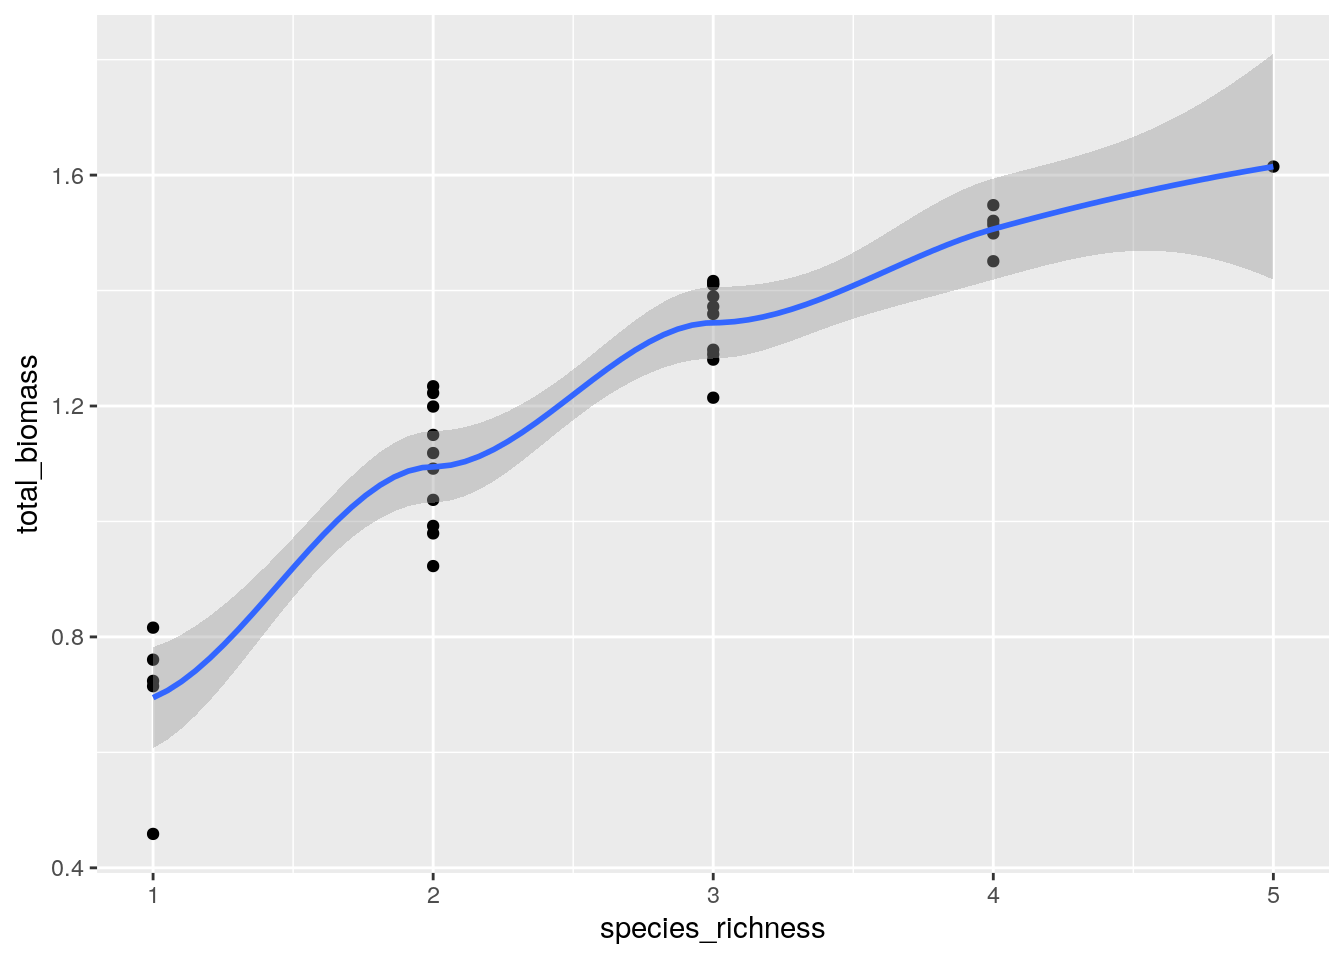
\includegraphics{A-Tour-of-the-Generalized-Lotka-Volterra-Model_files/figure-latex/glvbefplot-1} \end{center}

showing a modest increase in total biomass with increasing species richness.

\hypertarget{hyperplanes}{%
\section{Hyperplanes}\label{hyperplanes}}

We can rewrite the GLV model as:

\[
\begin{aligned}
\dfrac{dx(t)}{dt} &= D(x(t))(r + A x(t))\\
&= D(r x(t))(1 + B x(t))
\end{aligned}
\]
where we have \(b_{ij} = a_{ij} / r_i\). The equilibrium for each subset of species \(k\) (if it exists) can be found as \((B^{(k)})^{-1} 1^{(k)}\), where \((B^{(k)})^{-1}\) is the inverse of the \(B^{(k)}\) sub-matrix of \(B\) in which only the rows/columns belonging to \(k\) are retained, and \(1^{(k)}\) is a vector of ones with length equal to the number of species in \(k\).

We now want to link the matrix \(B\) with the results of the experiments, stored in matrix \(E\). Call \(x^{(k)}_i\) the recorded density of taxon \(i\) in community \(k\) (i.e., stored in one of the rows of \(E\)). Then, we can build a matrix \(P\) where each row represents an equation \(\sum_j b_{ij} x_j^{(k)} = 1\) and we have a column for each coefficient in \(B\). For example, take three taxa, and suppose that we can culture each in isolation, and that the all assemblages coexist when co-cultured. We can write 12 equations: monocultures (\(k \in \{1, 2, 4\}\)) give rise to a single equation; co-cultures of two taxa to two equations each (\(k \in \{3, 5, 6 \}\)); and communities with three taxa to three independent equations (\(k = 7\)). Here are the 12 equations we can write:

\[
\begin{aligned}
b_{11} x_1^{(1)} &= 1\\
b_{22} x_2^{(2)} &= 1\\
b_{11} x_1^{(3)} + b_{12}x_2^{(3)} &= 1\\
b_{21} x_1^{(3)} + b_{22}x_2^{(3)} &= 1\\
b_{33} x_3^{(4)} &= 1\\
b_{11} x_1^{(5)} + b_{13} x_3^{(5)} &= 1\\
b_{31} x_1^{(5)} + b_{33} x_3^{(5)} &= 1\\
b_{22} x_2^{(6)} + b_{23} x_3^{(6)} &= 1\\
b_{32} x_2^{(6)} + b_{33} x_3^{(6)} &= 1\\
b_{11} x_1^{(7)} + b_{12} x_2^{(7)} + b_{13} x_3^{(7)} & = 1\\
b_{21} x_1^{(7)} + b_{22} x_2^{(7)} + b_{23} x_3^{(7)} & = 1\\
b_{31} x_1^{(7)} + b_{32} x_2^{(7)} + b_{33} x_3^{(7)} & = 1
\end{aligned}
\]

We can summarize the equations in a more compact form as \(P v(B)=1\):

\[
\begin{pmatrix}
x_1^{(1)} & 0 & 0 & 0 & 0 & 0 & 0 & 0 & 0 \\
0 & 0 & 0 & 0 & x_2^{(2)} & 0 & 0 & 0 & 0 \\
x_1^{(3)} & x_2^{(3)} & 0 & 0 & 0 & 0 & 0 & 0 & 0 \\
0 & 0 & 0 & x_1^{(3)} & x_2^{(3)} & 0 & 0 & 0 & 0 \\
0 & 0 & 0 & 0 & 0 & 0 & 0 & 0 & x_3^{(4)} \\
x_1^{(5)} & 0 & x_3^{(5)} & 0 & 0 & 0 & 0 & 0 & 0 \\
0 & 0 & 0 & 0 & 0 & 0 & x_1^{(5)} & 0 & x_3^{(5)} \\
0 & 0 & 0 & 0 & x_2^{(6)} & x_3^{(6)} & 0 & 0 & 0 \\
0 & 0 & 0 & 0 & 0 & 0 & 0 & x_2^{(6)} & x_3^{(6)}\\
x_1^{(7)} & x_2^{(7)} & x_3^{(7)} & 0 & 0 & 0 & 0 & 0 & 0 \\
0 & 0 & 0 & x_1^{(7)} & x_2^{(7)} & x_3^{(7)} & 0 & 0 & 0 \\
0 & 0 & 0 & 0 & 0 & 0 & x_1^{(7)} & x_2^{(7)} & x_3^{(7)} 
\end{pmatrix}
\begin{pmatrix}
b_{11}\\
b_{12}\\
b_{13}\\
b_{21}\\
b_{22}\\
b_{23}\\
b_{31}\\
b_{32}\\
b_{33}
\end{pmatrix} 
= 
\begin{pmatrix}
1\\
1\\
1\\
1\\
1\\
1\\
1\\
1\\
1\\
1\\
1\\
1
\end{pmatrix}
\]
where \(v(B)\) is a vectorized version of \(B\). Because we have \(n 2^{n-1} = 12\) equations, and \(n^2 = 9\) variables, in principle the system can be solved. One can recognize the equation above as a linear regression, and choose \(\hat{v}(B) = P^{+}1\) (where \(P^{+}\) is the Moore-Penrose pseudo-inverse of \(P\)). Before doing that, however, we can try to simplify the calculation by rearranging the rows of \(P\):

\[
\begin{pmatrix}
x_1^{(1)} & 0 & 0      & 0 & 0 & 0     & 0 & 0 & 0 \\
x_1^{(3)} & x_2^{(3)} & 0      & 0 & 0 & 0     & 0 & 0 & 0 \\
x_1^{(5)} & 0 & x_3^{(5)}       & 0 & 0 & 0     & 0 & 0 & 0 \\
x_1^{(7)} & x_2^{(7)} & x_3^{(7)} & 0 & 0 & 0     & 0 & 0 & 0 \\
0 & 0 & 0     & 0 & x_2^{(2)} & 0     & 0 & 0 & 0 \\
0 & 0 & 0     & x_1^{(3)} & x_2^{(3)} & 0     & 0 & 0 & 0 \\
0 & 0 & 0     & 0 & x_2^{(6)} & x_3^{(6)}     & 0 & 0 & 0 \\
0 & 0 & 0     & x_1^{(7)} & x_2^{(7)} & x_3^{(7)} & 0 & 0 & 0 \\
0 & 0 & 0      & 0 & 0 & 0     & 0 & 0 & x_3^{(4)} \\
0 & 0 & 0     & 0 & 0 & 0     & x_1^{(5)} & 0 & x_3^{(5)} \\
0 & 0 & 0     & 0 & 0 & 0        & 0 & x_2^{(6)} & x_3^{(6)}\\
0 & 0 & 0     & 0 & 0 & 0        & x_1^{(7)} & x_2^{(7)} & x_3^{(7)} 
\end{pmatrix} 
\begin{pmatrix}
b_{11}\\
b_{12}\\
b_{13}\\
b_{21}\\
b_{22}\\
b_{23}\\
b_{31}\\
b_{32}\\
b_{33}
\end{pmatrix} 
= 
\begin{pmatrix}
1\\
1\\
1\\
1\\
1\\
1\\
1\\
1\\
1\\
1\\
1\\
1
\end{pmatrix}
\]

Showing that the matrix \(P\) is block-diagonal, with blocks \(P_i = E_i\), where \(E_i\) is the matrix \(E\) in which only the rows in which species \(i\) is present are retained. As such, we can solve for the matrix \(B\) one row at a time:

\[
\begin{pmatrix}
x_1^{(1)} & 0 & 0 \\
x_1^{(3)} & x_2^{(3)} & 0 \\
x_1^{(5)} & 0 & x_3^{(5)} \\
x_1^{(7)} & x_2^{(7)} & x_3^{(7)} 
\end{pmatrix} 
\begin{pmatrix}
b_{11}\\
b_{12}\\
b_{13}
\end{pmatrix} 
= 
\begin{pmatrix}
1\\
1\\
1\\
1
\end{pmatrix}
\]

For example:

\begin{Shaded}
\begin{Highlighting}[]
\CommentTok{# rescaled matrix}
\NormalTok{B <-}\StringTok{ }\DecValTok{1} \OperatorTok{/}\StringTok{ }\NormalTok{r }\OperatorTok{*}\StringTok{ }\NormalTok{A}
\CommentTok{# now try to recover B from matrix E}
\NormalTok{fitted_B <-}\StringTok{ }\KeywordTok{matrix}\NormalTok{(}\DecValTok{0}\NormalTok{, n, n)}
\ControlFlowTok{for}\NormalTok{ (i }\ControlFlowTok{in} \DecValTok{1}\OperatorTok{:}\NormalTok{n)\{}
  \CommentTok{# take the matrix Ei}
\NormalTok{  Ei <-}\StringTok{ }\NormalTok{E[E[,i] }\OperatorTok{>}\StringTok{ }\DecValTok{0}\NormalTok{, , drop =}\StringTok{ }\OtherTok{FALSE}\NormalTok{]}
  \CommentTok{# solve for the row (MASS::ginv computes the pseudoinverse)}
\NormalTok{  fitted_B[i,] <-}\StringTok{ }\OperatorTok{-}\KeywordTok{rowSums}\NormalTok{(MASS}\OperatorTok{::}\KeywordTok{ginv}\NormalTok{(Ei))}
\NormalTok{\}}
\KeywordTok{ggplot}\NormalTok{(}\DataTypeTok{data =} \KeywordTok{tibble}\NormalTok{(}\DataTypeTok{real =} \KeywordTok{as.vector}\NormalTok{(B),}
                     \DataTypeTok{fitted =} \KeywordTok{as.vector}\NormalTok{(fitted_B))) }\OperatorTok{+}\StringTok{ }
\StringTok{  }\KeywordTok{aes}\NormalTok{(}\DataTypeTok{x =}\NormalTok{ real, }\DataTypeTok{y =}\NormalTok{ fitted) }\OperatorTok{+}\StringTok{ }\KeywordTok{geom_point}\NormalTok{() }\OperatorTok{+}\StringTok{ }
\StringTok{  }\KeywordTok{geom_abline}\NormalTok{(}\DataTypeTok{slope =} \DecValTok{1}\NormalTok{, }\DataTypeTok{intercept =} \DecValTok{0}\NormalTok{)}
\end{Highlighting}
\end{Shaded}

\begin{center}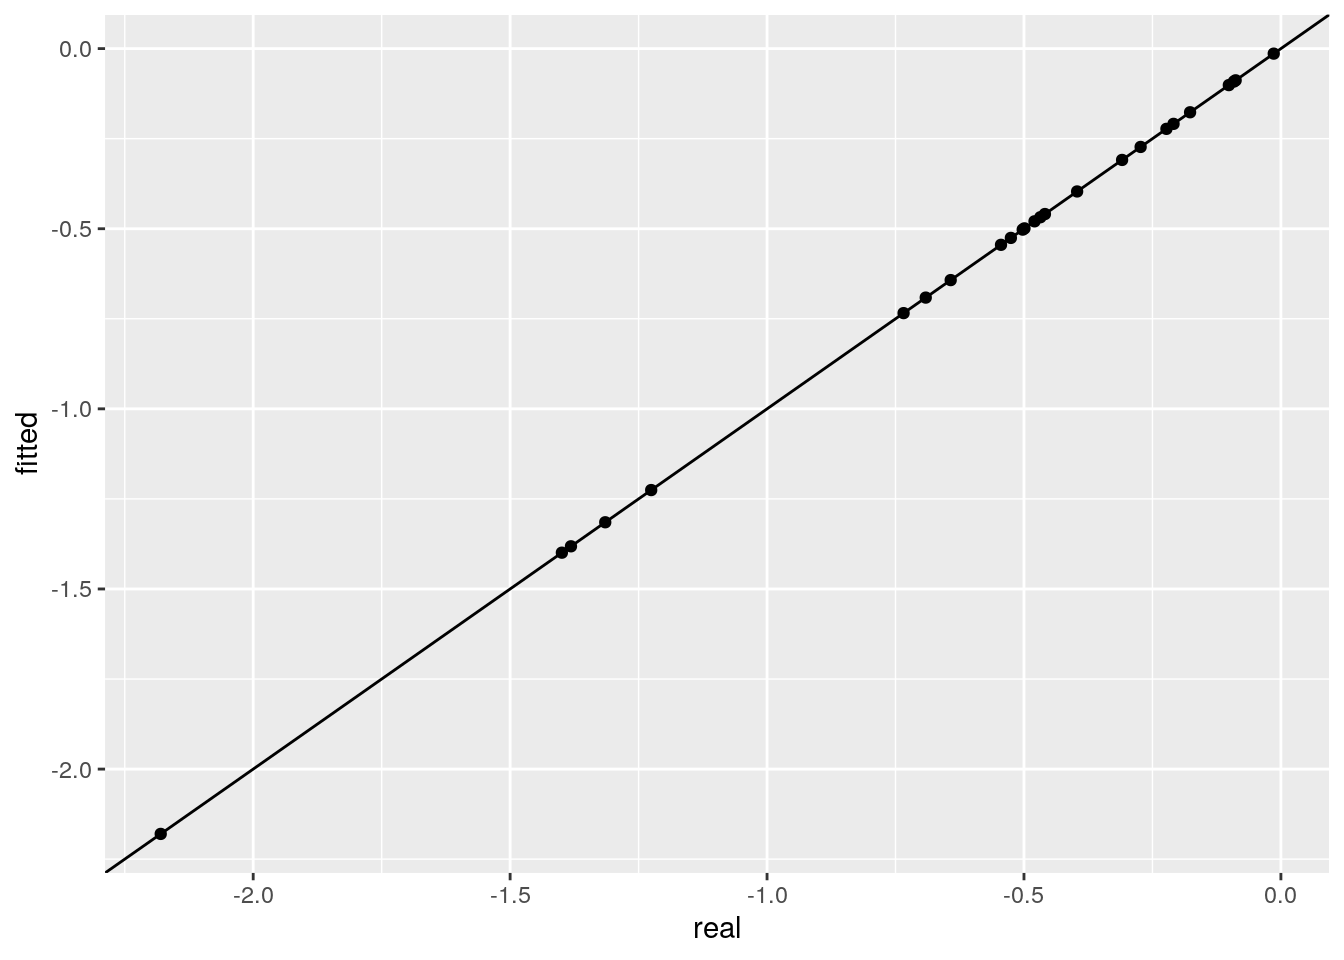
\includegraphics{A-Tour-of-the-Generalized-Lotka-Volterra-Model_files/figure-latex/examplefitendpoints-1} \end{center}

Notice that in general the system of equations is over-determined. As such, we can fit using a subset of the experiments, and then predict the rest of the experiments out-of-fit. For example, let's fit again using the information on monocultures and pairs only, and then predict experiment 31, in which all species should coexist:

\begin{Shaded}
\begin{Highlighting}[]
\NormalTok{E_partial <-}\StringTok{ }\NormalTok{E[}\KeywordTok{rowSums}\NormalTok{(E}\OperatorTok{>}\StringTok{ }\DecValTok{0}\NormalTok{) }\OperatorTok{<}\StringTok{ }\DecValTok{3}\NormalTok{, ]}
\NormalTok{fitted_B <-}\StringTok{ }\KeywordTok{matrix}\NormalTok{(}\DecValTok{0}\NormalTok{, n, n)}
\ControlFlowTok{for}\NormalTok{ (i }\ControlFlowTok{in} \DecValTok{1}\OperatorTok{:}\NormalTok{n)\{}
  \CommentTok{# take the matrix Ei}
\NormalTok{  Ei <-}\StringTok{ }\NormalTok{E_partial[E_partial[,i] }\OperatorTok{>}\StringTok{ }\DecValTok{0}\NormalTok{, , drop =}\StringTok{ }\OtherTok{FALSE}\NormalTok{]}
  \CommentTok{# solve for the row}
\NormalTok{  fitted_B[i,] <-}\StringTok{ }\OperatorTok{-}\KeywordTok{rowSums}\NormalTok{(MASS}\OperatorTok{::}\KeywordTok{ginv}\NormalTok{(Ei))}
\NormalTok{\}}
\KeywordTok{ggplot}\NormalTok{(}\DataTypeTok{data =} \KeywordTok{tibble}\NormalTok{(}\DataTypeTok{real =} \KeywordTok{as.vector}\NormalTok{(B),}
                     \DataTypeTok{fitted =} \KeywordTok{as.vector}\NormalTok{(fitted_B))) }\OperatorTok{+}\StringTok{ }
\StringTok{  }\KeywordTok{aes}\NormalTok{(}\DataTypeTok{x =}\NormalTok{ real, }\DataTypeTok{y =}\NormalTok{ fitted) }\OperatorTok{+}\StringTok{ }\KeywordTok{geom_point}\NormalTok{() }\OperatorTok{+}\StringTok{ }
\StringTok{  }\KeywordTok{geom_abline}\NormalTok{(}\DataTypeTok{slope =} \DecValTok{1}\NormalTok{, }\DataTypeTok{intercept =} \DecValTok{0}\NormalTok{)}
\end{Highlighting}
\end{Shaded}

\begin{center}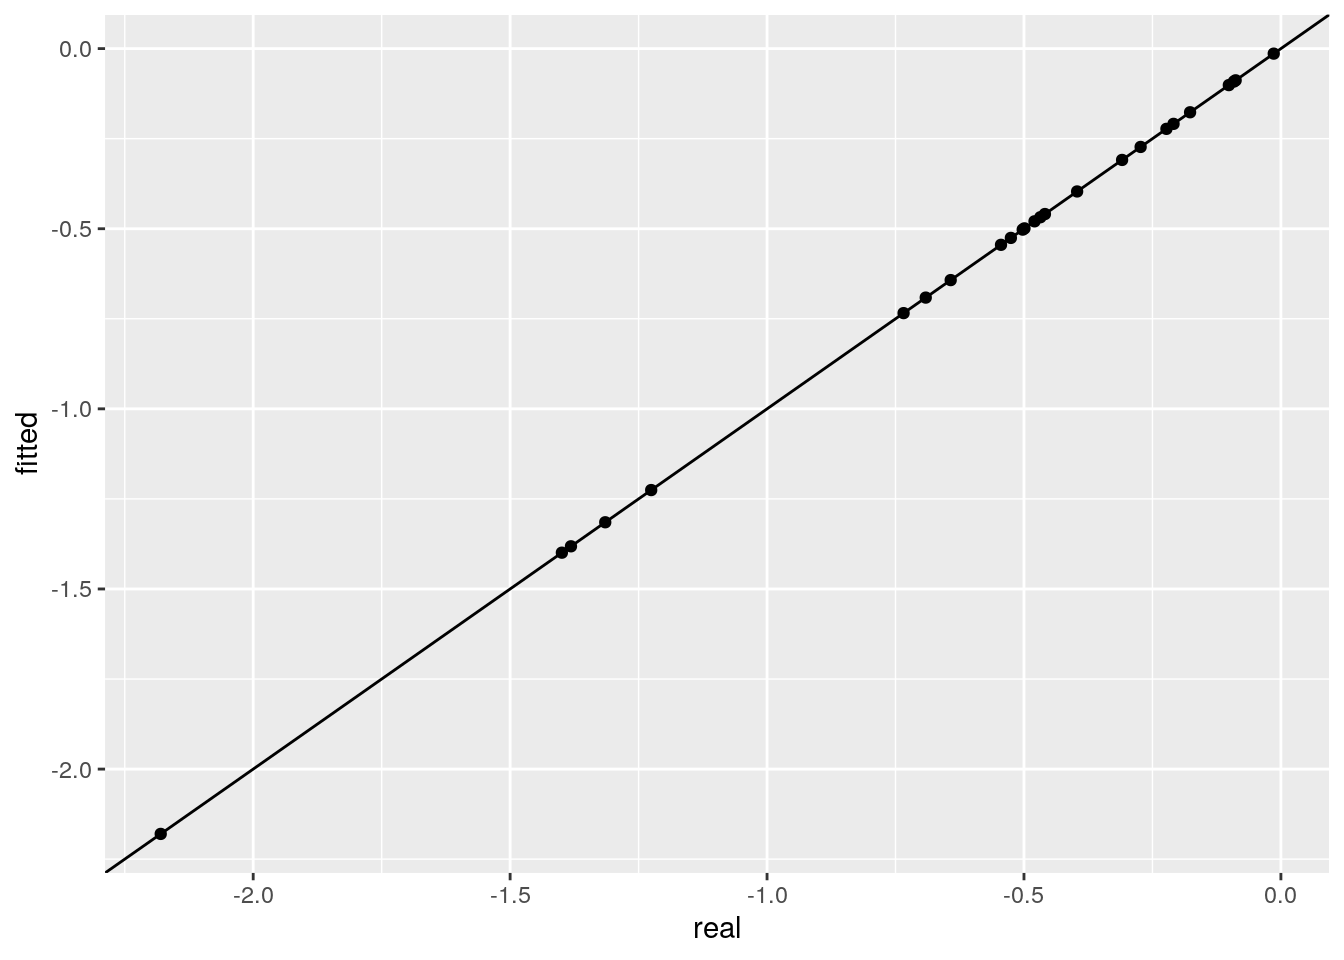
\includegraphics{A-Tour-of-the-Generalized-Lotka-Volterra-Model_files/figure-latex/examplefitendpoints2-1} \end{center}

\begin{Shaded}
\begin{Highlighting}[]
\KeywordTok{print}\NormalTok{(}\StringTok{"predicted"}\NormalTok{)}
\KeywordTok{solve}\NormalTok{(fitted_B, }\OperatorTok{-}\StringTok{ }\KeywordTok{rep}\NormalTok{(}\DecValTok{1}\NormalTok{, n))}
\KeywordTok{print}\NormalTok{(}\StringTok{"observed"}\NormalTok{)}
\NormalTok{E[(}\DecValTok{2}\OperatorTok{^}\NormalTok{n }\DecValTok{-1}\NormalTok{), ]}
\end{Highlighting}
\end{Shaded}

\begin{verbatim}
# [1] "predicted"
# [1] 0.4000232 0.3200119 0.5151320 0.1902248 0.1893434
# [1] "observed"
# [1] 0.4000232 0.3200119 0.5151320 0.1902248 0.1893434
\end{verbatim}

The equation \(E_i B_i = -1\) shows that all the equilibria of species \(i\) in a GLV system are arranged on a hyperplane.

\hypertarget{fitting-real-data}{%
\section{Fitting real data}\label{fitting-real-data}}

Having played with synthetic data, we can start thinking about data stemming from real experiments. In particular, consider the linear, additive model:

\[
x_i^{(k)} = \gamma_i - \sum_{j\neq i} \theta_{ij} x_i^{(k)}
\]
where \(x_i^{(k)}\) is the density of species \(i\) in community \(k\), \(\gamma_i\) models the density of \(i\) when grown in isolation, and the parameters \(\theta_{ij}\) how the density of \(i\) is influenced by the other species in community \(k\). Dividing both sides by \(\gamma_i\) and rearranging:

\[
\sum_{j\neq i} (\theta_{ij} /\gamma_i) x_i^{(k)} + (1/{\gamma_i}) x_i^{(k)}= \sum_j b_{ij} x_j^{(k)} = 1
\]
which is exactly the same system of equations found above. As such, fitting a linear, addittive model for the biomass of each species in each plot is equivalent to finding the equilibrium strcuture of a GLV model that approximates the data.

One thing to consider when modeling real data, contrary to simulated data, is the structure of the errors. For example, empirical data often contain replicates that reach slightly different densities. Moreover, what is typically done in these types of experiments is to sort and measure biomass for a section of each plot, and then to multiply to extrapolate the biomass for the whole plot. As such, if the error is normally distributed for the sub-plot, then it's going to be lognormally distributed for the whole plot. Furthermore, we need to link the rows of matrix \(P\) above, because when we make an error in measuring \(x_j^{(k)}\), the value is reported over several values. Following \citet{maynard2019predicting}, we do the following:

\begin{itemize}
\tightlist
\item
  Propose a matrix \(B\)
\item
  Compute the predicted abundance for all species in all observed assemblages (call them \(\tilde{x}_j^{(k)}\))
\item
  Compute the SSQ: \(\sum_{j, k} (\log x_j^{(k)} - \log \tilde{x}_j^{(k)})^2\)
\item
  Search numerically for the matrix \(B\) minimizing the SSQ
\end{itemize}

\begin{Shaded}
\begin{Highlighting}[]
\CommentTok{# constant to penalize solutions with negative}
\CommentTok{# abundances }
\NormalTok{penalization <-}\StringTok{ }\DecValTok{100000}
\CommentTok{# main fitting function}
\CommentTok{# input: }
\CommentTok{# - matrix E as above (the data)}
\CommentTok{# - proposed matrix B}
\CommentTok{# output:}
\CommentTok{# - predicted matrix \textbackslash{}tilde\{E\}}
\CommentTok{# - SSQ}
\NormalTok{compute_SSQ <-}\StringTok{ }\ControlFlowTok{function}\NormalTok{(B, E)\{}
\NormalTok{  tildeE <-}\StringTok{ }\NormalTok{E}
\NormalTok{  ones <-}\StringTok{ }\KeywordTok{rep}\NormalTok{(}\DecValTok{1}\NormalTok{, }\KeywordTok{ncol}\NormalTok{(B)) }\CommentTok{# vector of 1s}
  \ControlFlowTok{for}\NormalTok{ (i }\ControlFlowTok{in} \DecValTok{1}\OperatorTok{:}\KeywordTok{nrow}\NormalTok{(E))\{}
\NormalTok{    presence <-}\StringTok{ }\NormalTok{E[i, ] }\OperatorTok{>}\StringTok{ }\DecValTok{0}
    \CommentTok{# use internal calls to speed up calculation}
\NormalTok{    predicted_x <-}\StringTok{ }\KeywordTok{.Internal}\NormalTok{(}\KeywordTok{La_solve}\NormalTok{(B[presence, presence, }\DataTypeTok{drop =} \OtherTok{FALSE}\NormalTok{], }
\NormalTok{                                      ones[presence], }
                                      \DecValTok{10}\OperatorTok{^-}\DecValTok{6}\NormalTok{))}
\NormalTok{    tildeE[i, presence] <-}\StringTok{ }\NormalTok{predicted_x}
\NormalTok{  \}}
  \CommentTok{# now compute SSQ}
\NormalTok{  observed <-}\StringTok{ }\NormalTok{E[E }\OperatorTok{>}\StringTok{ }\DecValTok{0}\NormalTok{]}
  \CommentTok{# penalize negatives}
\NormalTok{  predicted <-}\StringTok{ }\NormalTok{tildeE[E }\OperatorTok{>}\StringTok{ }\DecValTok{0}\NormalTok{]}
\NormalTok{  predicted[predicted }\OperatorTok{<}\StringTok{ }\DecValTok{0}\NormalTok{] <-}\StringTok{ }\NormalTok{penalization}
  \KeywordTok{return}\NormalTok{(}\KeywordTok{list}\NormalTok{(}\DataTypeTok{B =}\NormalTok{ B, }
              \DataTypeTok{E =}\NormalTok{ E, }
              \DataTypeTok{tildeE =}\NormalTok{ tildeE, }
              \DataTypeTok{SSQ =} \KeywordTok{sum}\NormalTok{((}\KeywordTok{log}\NormalTok{(predicted) }\OperatorTok{-}\StringTok{ }\KeywordTok{log}\NormalTok{(observed))}\OperatorTok{^}\DecValTok{2}\NormalTok{)}
\NormalTok{              ))}
\NormalTok{\}}
\CommentTok{# for numerical minimization}
\NormalTok{to_minimize <-}\StringTok{ }\ControlFlowTok{function}\NormalTok{(b, E)\{}
\NormalTok{  n <-}\StringTok{ }\KeywordTok{ncol}\NormalTok{(E)}
  \KeywordTok{return}\NormalTok{(}\KeywordTok{compute_SSQ}\NormalTok{(}
    \KeywordTok{matrix}\NormalTok{(b, n, n),}
\NormalTok{    E}
\NormalTok{  )}\OperatorTok{$}\NormalTok{SSQ)}
\NormalTok{\}}
\end{Highlighting}
\end{Shaded}

To test this method, we are going to use the data from \citet{kuebbing2015above}, who co-cultured four species of plant in 14 out of 15 possible combinations. Let's load the data

\begin{Shaded}
\begin{Highlighting}[]
\NormalTok{url <-}\StringTok{ "https://github.com/dsmaynard/endpoints/raw/master/data/Kuebbing_plants/natives.csv"}
\NormalTok{E <-}\StringTok{ }\KeywordTok{as.matrix}\NormalTok{(}\KeywordTok{read_csv}\NormalTok{(url))}
\KeywordTok{head}\NormalTok{(E)}
\KeywordTok{tail}\NormalTok{(E)}
\end{Highlighting}
\end{Shaded}

\begin{verbatim}
#          as fa la po
# [1,] 1.4711  0  0  0
# [2,] 1.7968  0  0  0
# [3,] 1.8993  0  0  0
# [4,] 2.0634  0  0  0
# [5,] 2.2665  0  0  0
# [6,] 2.3062  0  0  0
#            as     fa     la     po
# [135,] 1.1219 1.8011 0.2390 1.4065
# [136,] 1.4751 1.3486 0.2474 1.5491
# [137,] 0.6021 1.9389 0.1817 2.7487
# [138,] 0.8973 1.6002 0.1156 3.2293
# [139,] 3.0384 1.4442 0.4590 1.5490
# [140,] 2.9240 2.3903 0.2379 4.3230
\end{verbatim}

And let's try to find a good numerical solution starting from the identity matrix:

\begin{Shaded}
\begin{Highlighting}[]
\KeywordTok{set.seed}\NormalTok{(}\DecValTok{2}\NormalTok{)}
\NormalTok{B <-}\StringTok{ }\KeywordTok{matrix}\NormalTok{(}\DecValTok{0}\NormalTok{, }\DecValTok{4}\NormalTok{, }\DecValTok{4}\NormalTok{)}
\KeywordTok{diag}\NormalTok{(B) <-}\StringTok{ }\DecValTok{1}
\NormalTok{tmp <-}\StringTok{ }\KeywordTok{optim}\NormalTok{(}\DataTypeTok{par =} \KeywordTok{as.vector}\NormalTok{(B), }
             \DataTypeTok{fn =}\NormalTok{ to_minimize, }
             \DataTypeTok{E =}\NormalTok{ E,}
             \DataTypeTok{method =} \StringTok{"BFGS"}\NormalTok{)}
\NormalTok{best_B <-}\StringTok{ }\KeywordTok{matrix}\NormalTok{(tmp}\OperatorTok{$}\NormalTok{par, }\DecValTok{4}\NormalTok{, }\DecValTok{4}\NormalTok{)}
\NormalTok{solution <-}\StringTok{ }\KeywordTok{compute_SSQ}\NormalTok{(best_B, E)}
\end{Highlighting}
\end{Shaded}

Now let's write code to show a nice plot of the predicted vs.~observed values for all communities:

\begin{Shaded}
\begin{Highlighting}[]
\NormalTok{plot_solution <-}\StringTok{ }\ControlFlowTok{function}\NormalTok{(solution)\{}
  \CommentTok{# add a column with community composition}
\NormalTok{  spnames <-}\StringTok{ }\KeywordTok{colnames}\NormalTok{(solution}\OperatorTok{$}\NormalTok{E)}
\NormalTok{  community <-}\StringTok{ }\KeywordTok{apply}\NormalTok{(solution}\OperatorTok{$}\NormalTok{E, }\DecValTok{1}\NormalTok{, }\ControlFlowTok{function}\NormalTok{(x) }\KeywordTok{paste}\NormalTok{(spnames[x }\OperatorTok{>}\StringTok{ }\DecValTok{0}\NormalTok{], }\DataTypeTok{collapse =} \StringTok{"_"}\NormalTok{))}
  \CommentTok{# work with observed data}
\NormalTok{  E <-}\StringTok{ }\KeywordTok{as_tibble}\NormalTok{(solution}\OperatorTok{$}\NormalTok{E) }\OperatorTok\StringTok{ }
\StringTok{    }\KeywordTok{add_column}\NormalTok{(}\DataTypeTok{community =}\NormalTok{ community) }\OperatorTok\StringTok{ }
\StringTok{    }\KeywordTok{mutate}\NormalTok{(}\DataTypeTok{experiment =} \KeywordTok{row_number}\NormalTok{())}
\NormalTok{  toplot <-}\StringTok{ }\NormalTok{E }\OperatorTok\StringTok{ }\KeywordTok{gather}\NormalTok{(species, observed_biomass, }\OperatorTok{-}\NormalTok{experiment, }\OperatorTok{-}\NormalTok{community) }\OperatorTok\StringTok{ }
\StringTok{    }\KeywordTok{filter}\NormalTok{(observed_biomass }\OperatorTok{>}\StringTok{ }\DecValTok{0}\NormalTok{)}
  \CommentTok{# now the predicted data}
\NormalTok{  tildeE <-}\StringTok{ }\KeywordTok{as_tibble}\NormalTok{(solution}\OperatorTok{$}\NormalTok{tildeE) }\OperatorTok
\StringTok{    }\KeywordTok{add_column}\NormalTok{(}\DataTypeTok{community =}\NormalTok{ community) }\OperatorTok\StringTok{ }
\StringTok{    }\KeywordTok{gather}\NormalTok{(species, predicted_biomass, }\OperatorTok{-}\NormalTok{community) }\OperatorTok\StringTok{ }
\StringTok{    }\KeywordTok{distinct}\NormalTok{()}
  \CommentTok{# join the two data sets}
\NormalTok{  toplot <-}\StringTok{ }\NormalTok{toplot }\OperatorTok\StringTok{ }
\StringTok{    }\KeywordTok{inner_join}\NormalTok{(tildeE, }\DataTypeTok{by =} \KeywordTok{c}\NormalTok{(}\StringTok{"community"}\NormalTok{, }\StringTok{"species"}\NormalTok{)) }\OperatorTok\StringTok{ }
\StringTok{    }\KeywordTok{filter}\NormalTok{(observed_biomass }\OperatorTok{>}\StringTok{ }\DecValTok{0}\NormalTok{)}
\NormalTok{  pl <-}\StringTok{ }\KeywordTok{ggplot}\NormalTok{(}\DataTypeTok{data =}\NormalTok{ toplot) }\OperatorTok{+}\StringTok{ }
\StringTok{    }\KeywordTok{aes}\NormalTok{(}\DataTypeTok{x =}\NormalTok{ species, }\DataTypeTok{fill =}\NormalTok{ species) }\OperatorTok{+}\StringTok{ }
\StringTok{    }\KeywordTok{geom_violin}\NormalTok{(}\KeywordTok{aes}\NormalTok{(}\DataTypeTok{y =}\NormalTok{ observed_biomass), }\DataTypeTok{draw_quantiles =} \FloatTok{0.5}\NormalTok{, }\DataTypeTok{scale =} \StringTok{"width"}\NormalTok{) }\OperatorTok{+}\StringTok{ }
\StringTok{    }\KeywordTok{geom_point}\NormalTok{(}\KeywordTok{aes}\NormalTok{(}\DataTypeTok{y =}\NormalTok{ predicted_biomass)) }\OperatorTok{+}\StringTok{ }
\StringTok{    }\KeywordTok{facet_wrap}\NormalTok{(}\OperatorTok{~}\NormalTok{community, }\DataTypeTok{scales =} \StringTok{"free_y"}\NormalTok{) }\OperatorTok{+}\StringTok{ }
\StringTok{    }\KeywordTok{scale_y_log10}\NormalTok{(}\StringTok{"biomass"}\NormalTok{)}
  \KeywordTok{return}\NormalTok{(pl)}
\NormalTok{\}}
\KeywordTok{plot_solution}\NormalTok{(solution)}
\end{Highlighting}
\end{Shaded}

\begin{center}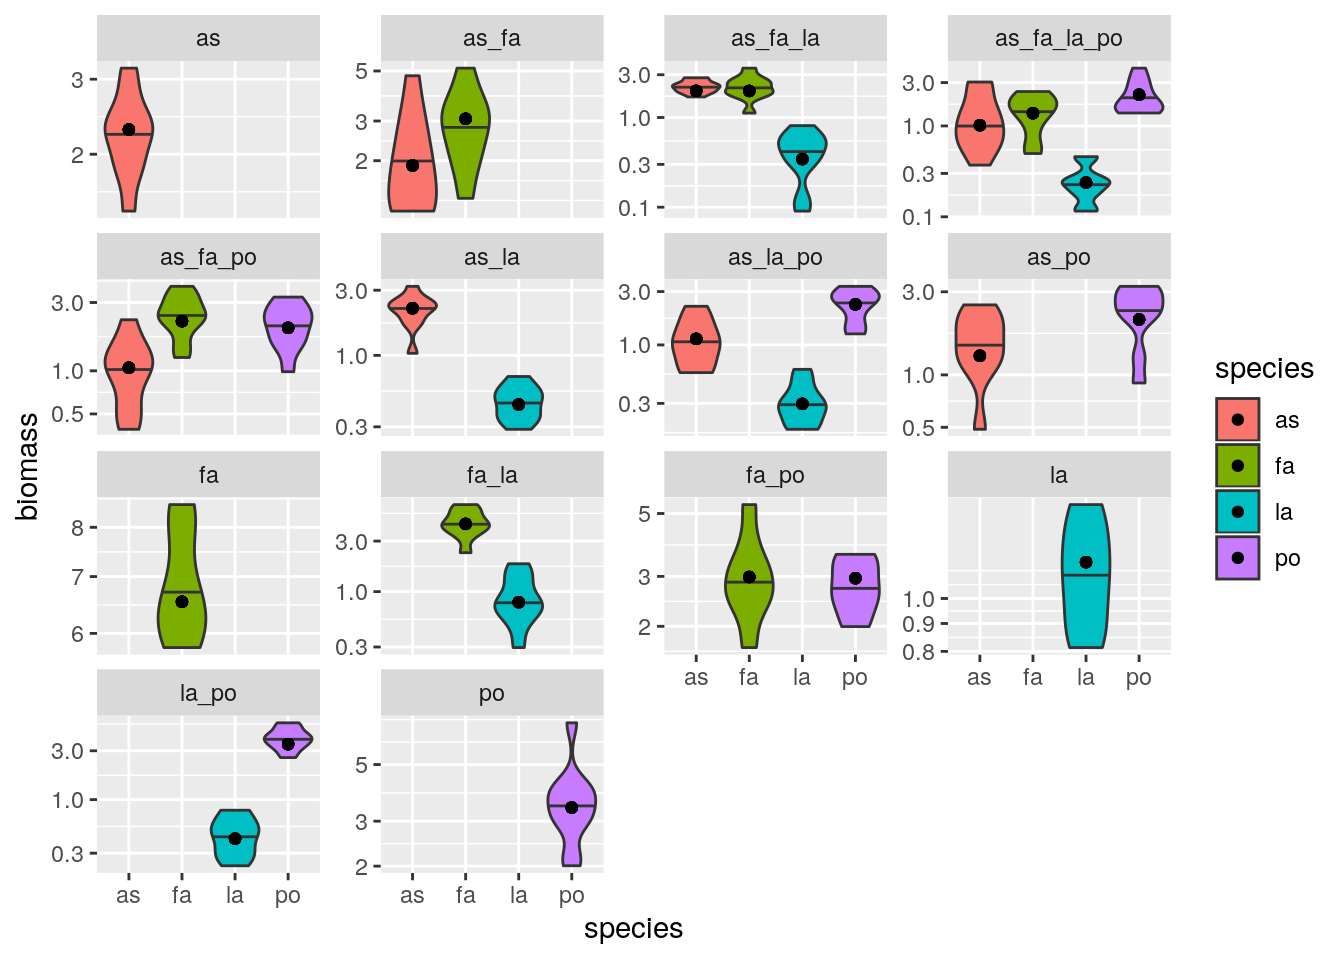
\includegraphics{A-Tour-of-the-Generalized-Lotka-Volterra-Model_files/figure-latex/plotendpoints-1} \end{center}

\hypertarget{predicting-real-data-out-of-fit}{%
\section{Predicting real data out of fit}\label{predicting-real-data-out-of-fit}}

Exactly as done for the GLV simulated data, we can attempt fitting the matrix \(B\) using only part of the experimental data, and then predict the rest out-of-fit. This is a powerful test to make sure that a) we have chosen a good structure for the statistical model, and b) we are not overfitting. For example, let's try to predict all triplets out of fit. First, we fit the model using only the information about monocultures, pairs, and the quadruplet (11 experiments); then, we use the fitted matrix to predict all of the data and plot:

\begin{Shaded}
\begin{Highlighting}[]
\KeywordTok{set.seed}\NormalTok{(}\DecValTok{1}\NormalTok{)}
\NormalTok{B <-}\StringTok{ }\KeywordTok{matrix}\NormalTok{(}\DecValTok{0}\NormalTok{, }\DecValTok{4}\NormalTok{, }\DecValTok{4}\NormalTok{)}
\KeywordTok{diag}\NormalTok{(B) <-}\StringTok{ }\DecValTok{1}
\NormalTok{Enotriplets <-}\StringTok{ }\NormalTok{E[}\KeywordTok{rowSums}\NormalTok{(E }\OperatorTok{>}\StringTok{ }\DecValTok{0}\NormalTok{) }\OperatorTok{!=}\StringTok{ }\DecValTok{3}\NormalTok{, ]}
\NormalTok{tmp <-}\StringTok{ }\KeywordTok{optim}\NormalTok{(}\DataTypeTok{par =} \KeywordTok{as.vector}\NormalTok{(B), }
             \DataTypeTok{fn =}\NormalTok{ to_minimize, }
             \DataTypeTok{E =}\NormalTok{ Enotriplets,}
             \DataTypeTok{method =} \StringTok{"BFGS"}\NormalTok{)}
\NormalTok{best_B_oof <-}\StringTok{ }\KeywordTok{matrix}\NormalTok{(tmp}\OperatorTok{$}\NormalTok{par, }\DecValTok{4}\NormalTok{, }\DecValTok{4}\NormalTok{)}
\NormalTok{solution_oof <-}\StringTok{ }\KeywordTok{compute_SSQ}\NormalTok{(best_B_oof, E)}
\KeywordTok{plot_solution}\NormalTok{(solution_oof)}
\end{Highlighting}
\end{Shaded}

\begin{center}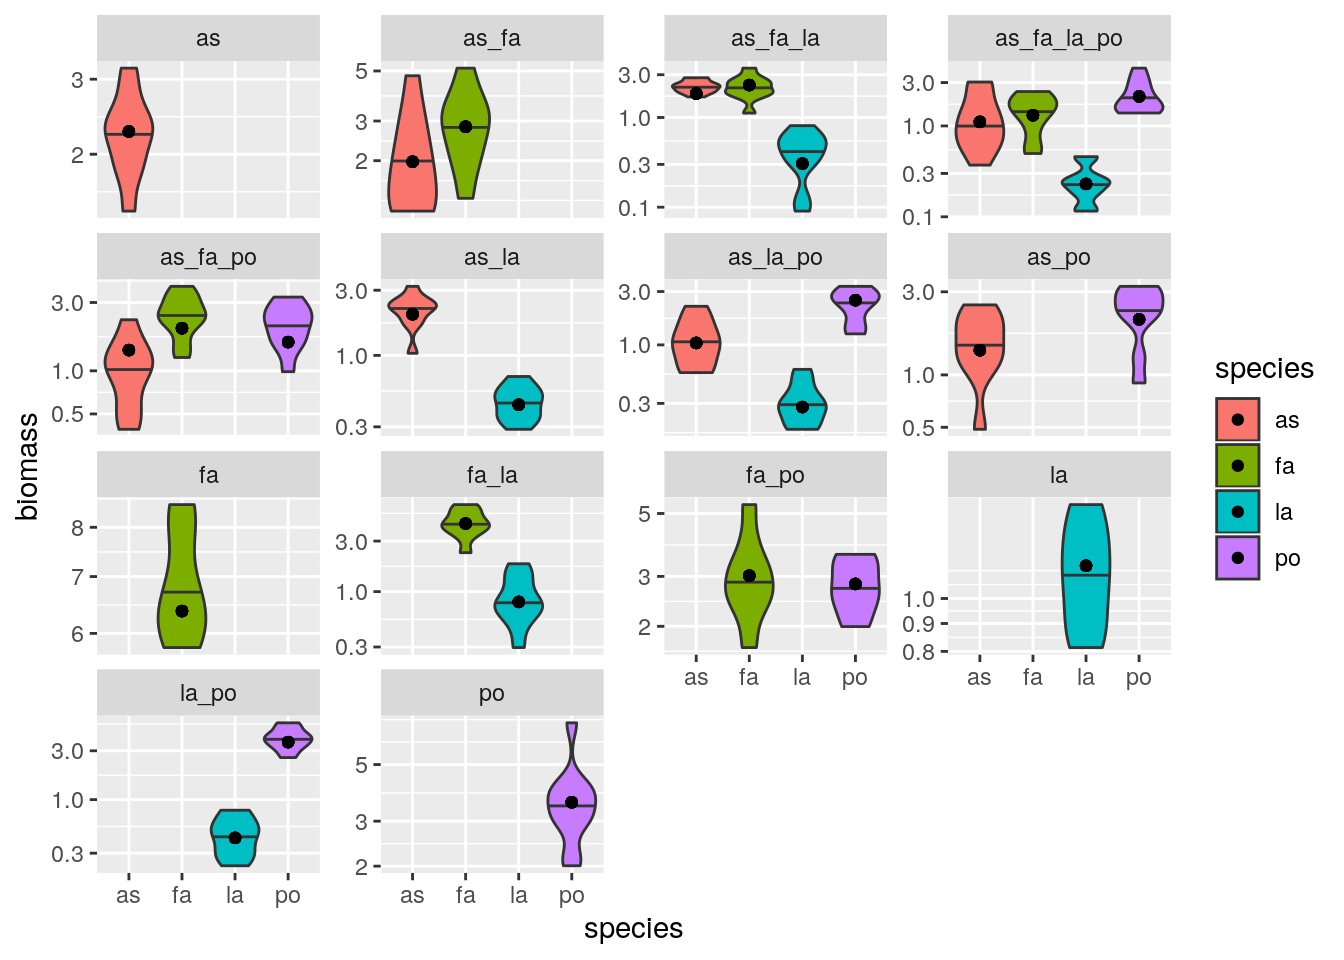
\includegraphics{A-Tour-of-the-Generalized-Lotka-Volterra-Model_files/figure-latex/kuebnumerics2-1} \end{center}

Repeat excluding all the pairs:

\begin{Shaded}
\begin{Highlighting}[]
\KeywordTok{set.seed}\NormalTok{(}\DecValTok{1}\NormalTok{)}
\NormalTok{B <-}\StringTok{ }\KeywordTok{matrix}\NormalTok{(}\DecValTok{0}\NormalTok{, }\DecValTok{4}\NormalTok{, }\DecValTok{4}\NormalTok{)}
\KeywordTok{diag}\NormalTok{(B) <-}\StringTok{ }\DecValTok{1}
\NormalTok{Enopairs <-}\StringTok{ }\NormalTok{E[}\KeywordTok{rowSums}\NormalTok{(E }\OperatorTok{>}\StringTok{ }\DecValTok{0}\NormalTok{) }\OperatorTok{!=}\StringTok{ }\DecValTok{2}\NormalTok{, ]}
\NormalTok{tmp <-}\StringTok{ }\KeywordTok{optim}\NormalTok{(}\DataTypeTok{par =} \KeywordTok{as.vector}\NormalTok{(B), }
             \DataTypeTok{fn =}\NormalTok{ to_minimize, }
             \DataTypeTok{E =}\NormalTok{ Enopairs,}
             \DataTypeTok{method =} \StringTok{"BFGS"}\NormalTok{)}
\NormalTok{best_B_oof2 <-}\StringTok{ }\KeywordTok{matrix}\NormalTok{(tmp}\OperatorTok{$}\NormalTok{par, }\DecValTok{4}\NormalTok{, }\DecValTok{4}\NormalTok{)}
\NormalTok{solution_oof2 <-}\StringTok{ }\KeywordTok{compute_SSQ}\NormalTok{(best_B_oof2, E)}
\KeywordTok{plot_solution}\NormalTok{(solution_oof2)}
\end{Highlighting}
\end{Shaded}

\begin{center}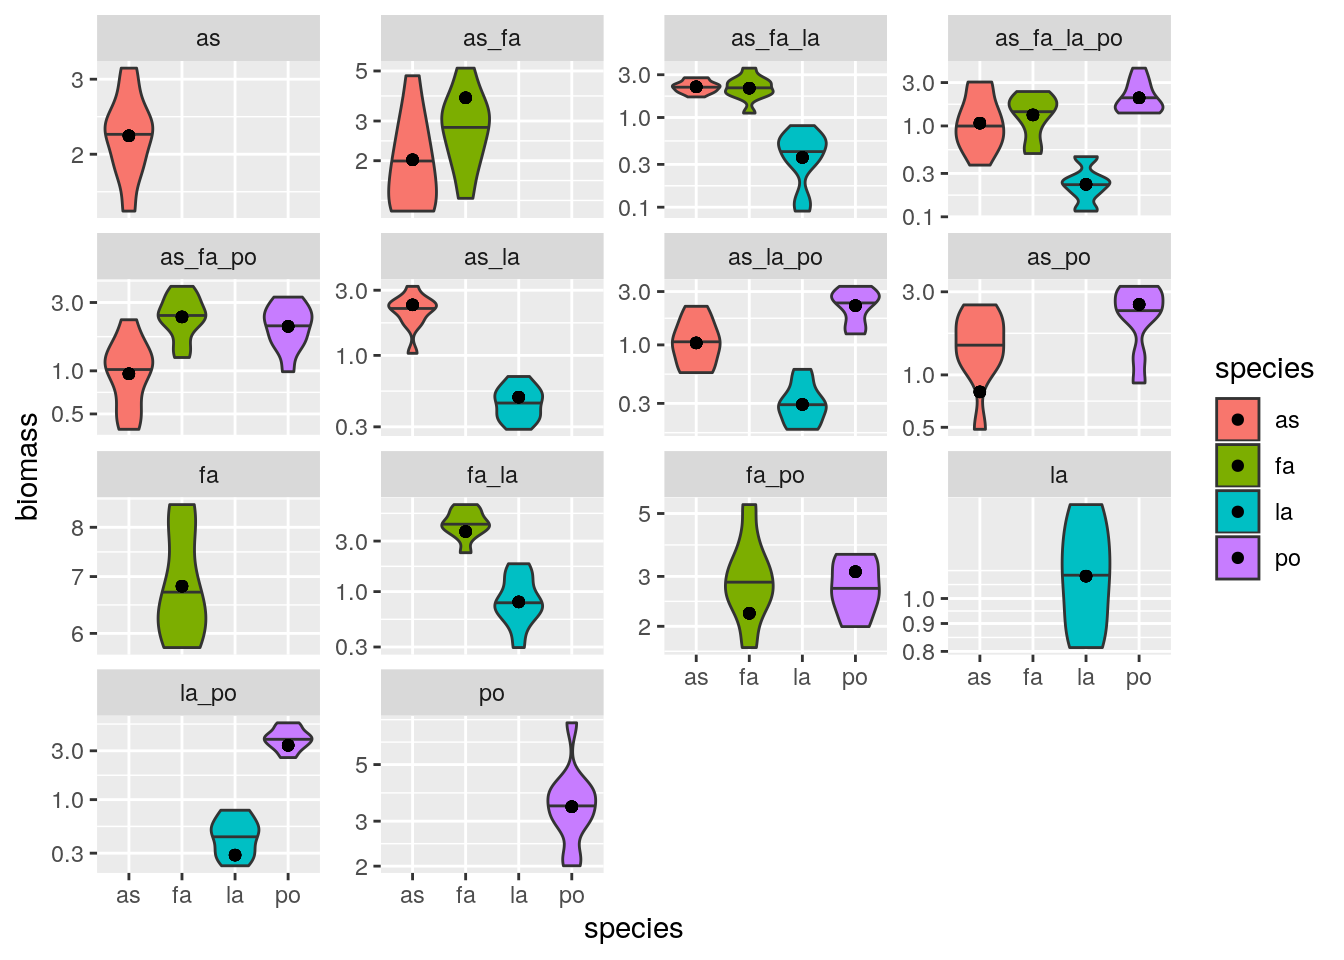
\includegraphics{A-Tour-of-the-Generalized-Lotka-Volterra-Model_files/figure-latex/kuebnumerics3-1} \end{center}

Of course, we might push this too far. For example, a popular way to attempt parameterizing models is to consider only monocultures and pairs:

\begin{Shaded}
\begin{Highlighting}[]
\KeywordTok{set.seed}\NormalTok{(}\DecValTok{1}\NormalTok{)}
\NormalTok{B <-}\StringTok{ }\KeywordTok{matrix}\NormalTok{(}\DecValTok{0}\NormalTok{, }\DecValTok{4}\NormalTok{, }\DecValTok{4}\NormalTok{)}
\KeywordTok{diag}\NormalTok{(B) <-}\StringTok{ }\DecValTok{1}
\NormalTok{Eonlymonopairs <-}\StringTok{ }\NormalTok{E[}\KeywordTok{rowSums}\NormalTok{(E }\OperatorTok{>}\StringTok{ }\DecValTok{0}\NormalTok{) }\OperatorTok{<}\StringTok{ }\DecValTok{3}\NormalTok{, ]}
\NormalTok{tmp <-}\StringTok{ }\KeywordTok{optim}\NormalTok{(}\DataTypeTok{par =} \KeywordTok{as.vector}\NormalTok{(B), }
             \DataTypeTok{fn =}\NormalTok{ to_minimize, }
             \DataTypeTok{E =}\NormalTok{ Eonlymonopairs,}
             \DataTypeTok{method =} \StringTok{"BFGS"}\NormalTok{)}
\NormalTok{best_B_oof3 <-}\StringTok{ }\KeywordTok{matrix}\NormalTok{(tmp}\OperatorTok{$}\NormalTok{par, }\DecValTok{4}\NormalTok{, }\DecValTok{4}\NormalTok{)}
\NormalTok{solution_oof3 <-}\StringTok{ }\KeywordTok{compute_SSQ}\NormalTok{(best_B_oof3, E)}
\KeywordTok{plot_solution}\NormalTok{(solution_oof3)}
\end{Highlighting}
\end{Shaded}

\begin{center}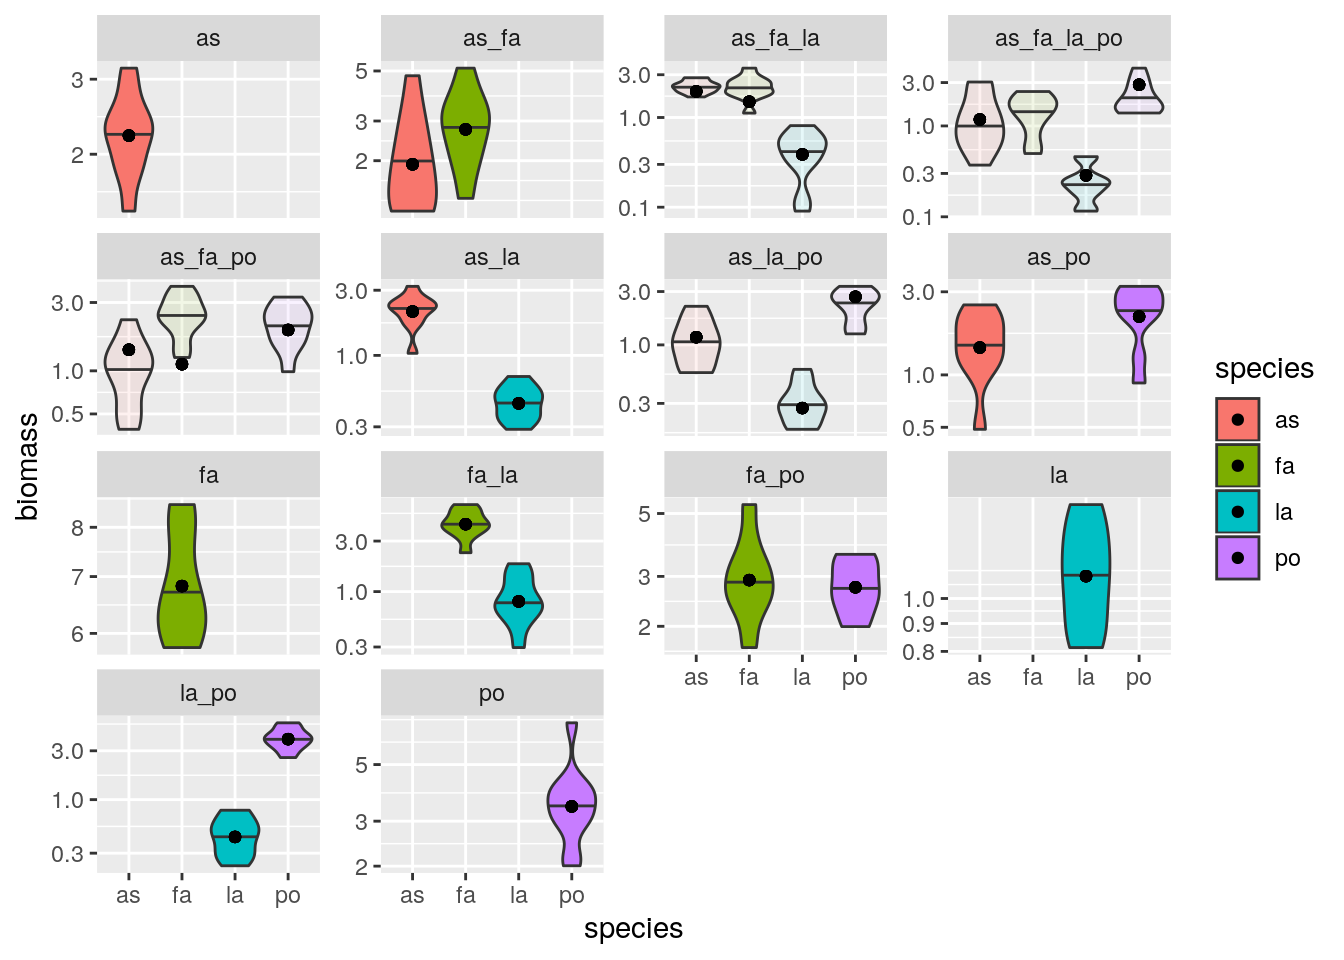
\includegraphics{A-Tour-of-the-Generalized-Lotka-Volterra-Model_files/figure-latex/kuebnumerics4-1} \end{center}

You can see that we predict a lack of coexistence for the system with all four species, while experimentally we have observed coexistence in all ten replicates. \citet{maynard2019predicting} have demonstrated that experimental designs mixing high- and low-abundance experiments provide the best fit while minimizing the number of experiments.

\bibliography{book.bib}


\end{document}
